\documentclass[
	12pt,				% tamanho da fonte
	openany,			% capítulos começam em pág ímpar (insere página vazia caso preciso)
	oneside, 			% oneside - twoside
	a4paper,			% tamanho do papel.
	chapter=TITLE,		% títulos de capítulos convertidos em letras maiúsculas
	section=TITLE,		% títulos de seções convertidos em letras maiúsculas
	sumario=tradicional,	
	%subsection=TITLE,	% títulos de subseções convertidos em letras maiúsculas
	%subsubsection=TITLE,% títulos de subsubseções convertidos em letras maiúsculas
	english,			% idioma adicional para hifenização
	brazil,				% o último idioma é o principal do documento
	]{abntex2}
	
	% ---------------------------------------------------------------------------
% Inclui os comandos do projeto
% ---------------------------------------------------------------------------
\usepackage{footmisc}
% this avoids resetting the footnote counter between chapters
\counterwithout*{footnote}{chapter}
% footnote spacing
\addtolength{\skip\footins}{1cm}

% -----------------------------------------------------------------------------
% Pacotes fundamentais
% -----------------------------------------------------------------------------
\usepackage{xcolor}
\newcommand\myworries[1]{\textcolor{red}{[#1]}}
\usepackage{lmodern}		% Usa a fonte Latin Modern (Serifada, tipo Times New Roman
%\usepackage{helvet}		% Usa a fonte Helvetica (Tipo Arial)	
%\renewcommand{\familydefault}{\sfdefault} tira o serifado
\usepackage[T1]{fontenc}		% Selecao de codigos de fonte.
\usepackage[utf8]{inputenc}		% Codificacao do documento (conversão automática dos acentos)
\usepackage{indentfirst}		% Indenta o primeiro parágrafo de cada seção.
\usepackage{color}				% Controle das cores
\usepackage{tikz}				% Inclusão de gráficos
\usepackage{graphicx}			% Inclusão de gráficos
\usepackage{microtype} 			% para melhorias de justificação
% -----------------------------------------------------------------------------
% Pacotes adicionais, usados no anexo do modelo de folha de identificação
% -----------------------------------------------------------------------------
\usepackage{multicol}
\usepackage{multirow}
% -----------------------------------------------------------------------------
% Pacotes adicionais, usados apenas no âmbito do Modelo Canônico do abnteX2
% -----------------------------------------------------------------------------
\usepackage{lipsum}				% para geração de dummy text
% -----------------------------------------------------------------------------
% Pacotes de citações
% -----------------------------------------------------------------------------
\usepackage[brazilian,hyperpageref]{backref}	 % Paginas com as citações na bibliografia
\usepackage[alf,abnt-etal-list=3,abnt-etal-cite=3, abnt-emphasize=bf]{abntex2cite}	% Citações padrão ABNT
\usepackage{pdflscape}
\usepackage{footnote}
\usepackage{pdfpages}
\usepackage{caption}

% -----------------------------------------------------------------------------
% Pacotes adicionados por @leolleocomp
% ----------------------------------------------------------------------------- 
\usepackage{booktabs}
\usepackage{adjustbox}
\usepackage{subcaption}
\usepackage[labelfont=bf]{caption}
\usepackage{gensymb}
\usepackage{amsmath}
\usepackage{array}
\usepackage{float}
\usepackage{xcolor,colortbl}
\usepackage{longtable}
\usepackage{scalefnt}
\usepackage{listings}			% inserir codigo fonte


% -----------------------------------------------------------------------------
% Pacotes adicionados por @Gabrielr2508
% ----------------------------------------------------------------------------- 
\usepackage{hyperref}

\usepackage{tocloft}
% -- permite a adição de células especiais em tabelas
\newcommand{\specialcell}[2][c]{%
  \begin{tabular}[#1]{@{}c@{}}#2\end{tabular}}

\newcounter{equationset}
\newcommand{\equationset}[1]{% \equationset{<caption>}
  \refstepcounter{equationset}% Step counter
  \noindent\makebox[\linewidth]{Equação ~\theequationset: #1}
 }

%--------------------------------------------------------------------------------
% Adequação dos títulos dos capitulos, seções, subseções às normas da Univasf
% Added by @Gabrielr2508
%--------------------------------------------------------------------------------
\renewcommand{\ABNTEXchapterfont}{\fontseries{b}}
\renewcommand{\ABNTEXchapterfontsize}{\normalsize}

\renewcommand{\ABNTEXsectionfont}{\fontseries{m}}
\renewcommand{\ABNTEXsectionfontsize}{\normalsize}

\renewcommand{\ABNTEXsubsectionfont}{\fontseries{b}}
\renewcommand{\ABNTEXsubsectionfontsize}{\normalsize}

\renewcommand{\ABNTEXsubsubsectionfont}{\fontseries{m}}
\renewcommand{\ABNTEXsubsubsectionfontsize}{\normalsize}

%--------------------------------------------------------------------------------
% CONFIGURAÇÕES DE PACOTES
% Configurações do pacote backref
%--------------------------------------------------------------------------------
% Usado sem a opção hyperpageref de backref
\renewcommand{\backrefpagesname}{Citado na(s) página(s):~}
% Texto padrão antes do número das páginas
\renewcommand{\backref}{}
% Define os textos da citação
\renewcommand*{\backrefalt}[4]{
	\ifcase #1 %
		%Nenhuma citação no texto.%
	\or
		Citado na página #2.%
	\else
		Citado #1 vezes nas páginas #2.%
	\fi}%

%--------------------------------------------------------------------------------
% Configurações de aparência do PDF final
%--------------------------------------------------------------------------------
% alterando o aspecto da cor azul
\definecolor{blue}{RGB}{41,5,195}

% informações do PDF
\makeatletter
\hypersetup{
     	%pagebackref=true,
		pdftitle={\@title},
		pdfauthor={\@author},
    	pdfsubject={\imprimirpreambulo},
	    pdfcreator={LaTeX with abnTeX2},
		pdfkeywords={abnt}{latex}{abntex}{abntex2}{relatório técnico},
		colorlinks=true,			% false: boxed links; true: colored links
    	linkcolor=black,				% color of internal links
    	citecolor=black,				% color of links to bibliography
    	filecolor=black,			% color of file links
		urlcolor=black,
		bookmarksdepth=4
}
\makeatother
% ---

% ---
% Espaçamentos entre linhas e parágrafos
% ---

% O tamanho do parágrafo é dado por:
\setlength{\parindent}{1.3cm}

% Controle do espaçamento entre um parágrafo e outro:
\setlength{\parskip}{0.2cm}  % tente também \onelineskip

%--------------------------------------------------------------------------------
% compila o indice
%--------------------------------------------------------------------------------
\makeindex
% ---

%--------------------------------------------------------------------------------
% Comando para inserir imagens de forma simples
%--------------------------------------------------------------------------------
\newcommand{\imagem}[4]
{%			\imagem{x.x}{nomeimg}{titulo}{fonte}
	\begin{figure}[!htb]
		\caption{\label{img:#2}#3}
		\begin{center}
			\includegraphics[scale=#1]{img/#2}
		\end{center}
        \legend{\textbf{Fonte:} #4}
	\end{figure}
}%

%--------------------------------------------------------------------------------
% Creio que esses comandos sejam para desenhar algo, aguardando explicações de @leolleocomp
%--------------------------------------------------------------------------------
\newcommand{\xx} {$\bigotimes$}
\newcommand{\oo} {$\bigcirc$}

%--------------------------------------------------------------------------------
% Biblioteca para códigos-fonte
%--------------------------------------------------------------------------------
\usepackage[newfloat=true]{minted}

%--------------------------------------------------------------------------------
% Caixas batutas - by @leolleocomp
%--------------------------------------------------------------------------------
\usepackage[most]{tcolorbox}
\tcbuselibrary{breakable}

\tcbuselibrary{minted}
\tcbset{listing engine=minted}

\definecolor{bg}{rgb}{0.95,0.95,0.95}

\SetupFloatingEnvironment{listing}{name=Código, listname=Lista de códigos}

%--------------------------------------------------------------------------------
% configuração do contador dos códigos-fonte - by @leolleocomp
% assim como as figuras, começa em 1
\newcounter{sourcecode}
%--------------------------------------------------------------------------------
%--------------------------------------------------------------------------------
% @leolleocomp
% stackoverflow code
% peguei da resposta abaixo
% https://stackoverflow.com/questions/24086366/change-latex-minted-listings-numbering-to-include-current-section?answertab=votes#tab-top
%--------------------------------------------------------------------------------
\makeatletter
\renewcommand*{\thelisting}{\thesourcecode}
\makeatother

%--------------------------------------------------------------------------------
% Peçam explicações a @leolleo
% WHO DID THIS?
%--------------------------------------------------------------------------------
\newcommand{\Ididthis}{
%	\legend{\textbf{Fonte:} O autor (\the\year).}
\legend{\textbf{Fonte:} O autor}
}

\newcommand{\Otherguydidthis}[1]{
	\legend{\textbf{Fonte:} \citeonline{#1}.}
}

%--------------------------------------------------------------------------------
% Comando para inserir códigos - by @leolleocomp
%--------------------------------------------------------------------------------
\newcommand{\sourcecode}[4]{
\begin{listing}[H]
	\refstepcounter{sourcecode}
	\caption{#1}
	\label{cmd:#2}
	\inputminted[linenos, bgcolor=bg, tabsize=4,breaklines]{#3}{codes/#4}
	\Ididthis
\end{listing}
}



% ---------------------------------------------------------------------------
% IDENTIFICAÇÃO
% ---------------------------------------------------------------------------
\titulo{DETERMINAÇÃO DE SÓLIDOS SOLÚVEIS TOTAIS EM MANGAS PALMER ATRAVÉS DE PROCESSAMENTO DIGITAL DE IMAGENS}
\autor{DANIELE SILVA REIS}
\local{JUAZEIRO - BA}
\orientador{Prof. Dr. Rosalvo Ferreira de Oliveira Neto}
\coorientador[Co-Orientadora: ]{M. Sc.ª Josenara Daiane de Souza Costa}
\instituicao{
UNIVERSIDADE FEDERAL DO VALE DO SÃO FRANCISCO
	\par
CURSO DE GRADUAÇÃO EM ENGENHARIA DE COMPUTAÇÃO}
\tipotrabalho{Trabalho de Conclusão de Curso}
\preambulo{Trabalho apresentado à Universidade Federal do Vale do São Francisco - Univasf, Campus Juazeiro, como requisito da obtenção do título de Bacharel em Engenharia de Computação.}


% -----------------------------------------------------------------------------
% CONFIGURACAO DO SUMARIO - by @Gabrielr2508
% Precisa estar aqui, por isso não foi para o commands.tex, não descobrimos o motivo, %caso saiba, por favor, faça um pull request! :D
% -----------------------------------------------------------------------------
% Secao primaria (Chapter) Caixa alta, Negrito, tamanho 12
\makeatletter
\renewcommand*{\l@chapter}[2]{%
  \l@chapapp{\uppercase{#1}}{#2}{\cftchaptername}}
\makeatother
% Secao secundaria (Section) Caixa baixa, Negrito, tamanho 12
\renewcommand{\cftsectionfont}{\uppercase} %ponha \rmfamily se quiser serifadas...

% Secao terciaria (Subsection) Caixa baixa, negrito, tamanho 12
\renewcommand{\cftsubsectionfont}{\bfseries}

% Secao quaternaria (Subsubsection) Caixa baixa, tamanho 12
\renewcommand{\cftsubsubsectionfont}{\normalfont}

% Seção quinaria (subsubsubsection) Caixa baixa, sem negrito, tamanho 12
\renewcommand{\cftparagraphfont}{\normalfont\itshape}


% -----------------------------------------------------------------------------
% Início do TCC 
% -----------------------------------------------------------------------------
\begin{document}

	\frenchspacing % Retira espaço extra obsoleto entre as frases.
	
	\pretextual
		%--------------------------------------------------------------------------------
% Constrói a capa com base na seção de identificação do main.tex
%--------------------------------------------------------------------------------
\begin{capa}
\center
	
\includegraphics[scale=0.6]{img/univasf.jpg}

	{\ABNTEXchapterfont\bfseries\large\imprimirinstituicao}

	\vspace*{5cm}
	{\ABNTEXchapterfont\bfseries\large\imprimirautor}

	\vfill
	{\ABNTEXchapterfont\bfseries\large\imprimirtitulo}
	\vfill
	\ABNTEXchapterfont\bfseries\large\imprimirlocal\\ \the\year

	\vspace*{1cm}

\end{capa}
%--------------------------------------------------------------------------------
% Constrói a folha de rosto com base na seção de identificação do main.tex
%--------------------------------------------------------------------------------
\begin{folhaderosto}
\center
		{\ABNTEXchapterfont\bfseries\large\imprimirautor}
		\vspace*{\fill}

		{\ABNTEXchapterfont\bfseries\large\imprimirtitulo}
		\vspace*{\fill}

		{\hspace{.45\textwidth}
		\begin{minipage}{.5\textwidth}
			\SingleSpacing
			\imprimirpreambulo \\ \\

			{\imprimirorientadorRotulo~\imprimirorientador\par}
			{\imprimircoorientadorRotulo~\imprimircoorientador\par}

		\end{minipage}%
		\vspace*{\fill}}%
		\vspace*{\fill}
			\ABNTEXchapterfont\bfseries\large\imprimirlocal\\ \the\year
		\vspace*{1cm}
\end{folhaderosto}

%--------------------------------------------------------------------------------
% Constrói a ficha catalográfia com base na seção de identificação do main.tex
% Está comentado porque no final das contas a biblioteca do seu campus que gera a 
% numeração, você pode adicionar os numeros aqui, ou anexar o pdf gerado por eles
% ao documento.
%--------------------------------------------------------------------------------
%\begin{fichacatalografica}
%	\vspace*{\fill}					% Posição vertical
%	\hrule							% Linha horizontal
%	\begin{center}					% Minipage Centralizado
%	\begin{minipage}[c]{12.5cm}		% Largura
%
%	\imprimirautor
%
%	\hspace{0.5cm} \imprimirtitulo  / \imprimirautor. --
%	\imprimirlocal, \the\year-
%
%	\hspace{0.5cm} xx p. : il. (algumas color.) ; 30 cm.\\
%
%	\hspace{0.5cm} \imprimirorientadorRotulo~\imprimirorientador\\
%
%	\hspace{0.5cm}
%	\parbox[t]{\textwidth}{\imprimirtipotrabalho~--~\imprimirinstituicao,
%	\the\year.}\\
%
%	\hspace{0.5cm}
%		1. Palavra-chave1.
%		2. Palavra-chave2.
%		I. Orientador.
%		II. Universidade xxx.
%		III. Faculdade de xxx.
%		IV. Título\\
%
%	\hspace{8.75cm} CDU 02:141:005.7\\
%
%	\end{minipage}
%	\end{center}
%	\hrule
%\end{fichacatalografica}

%--------------------------------------------------------------------------------
% Anexando a ficha catalogáfica e a folha de aprovação 
%--------------------------------------------------------------------------------
% 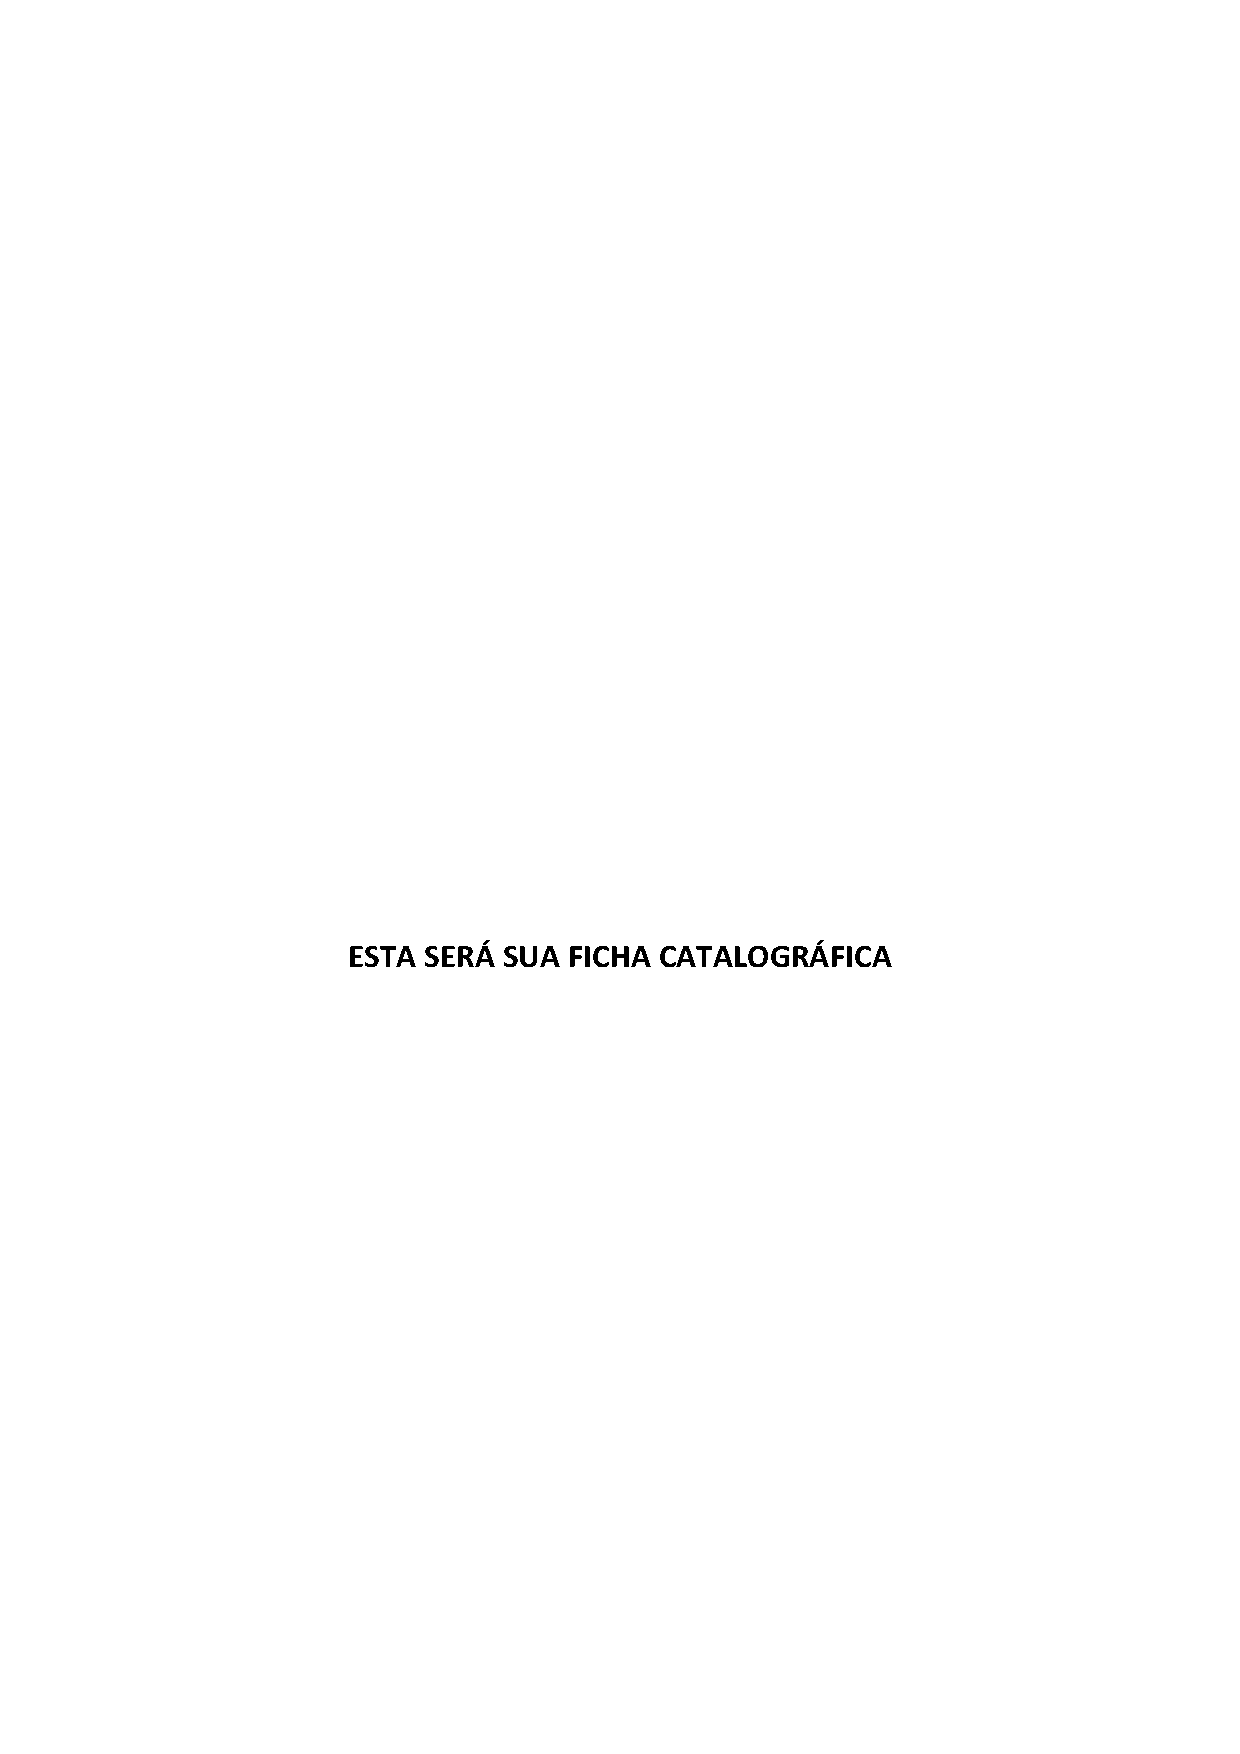
\includepdf[pages=-]{anexos/ficha.pdf}

% 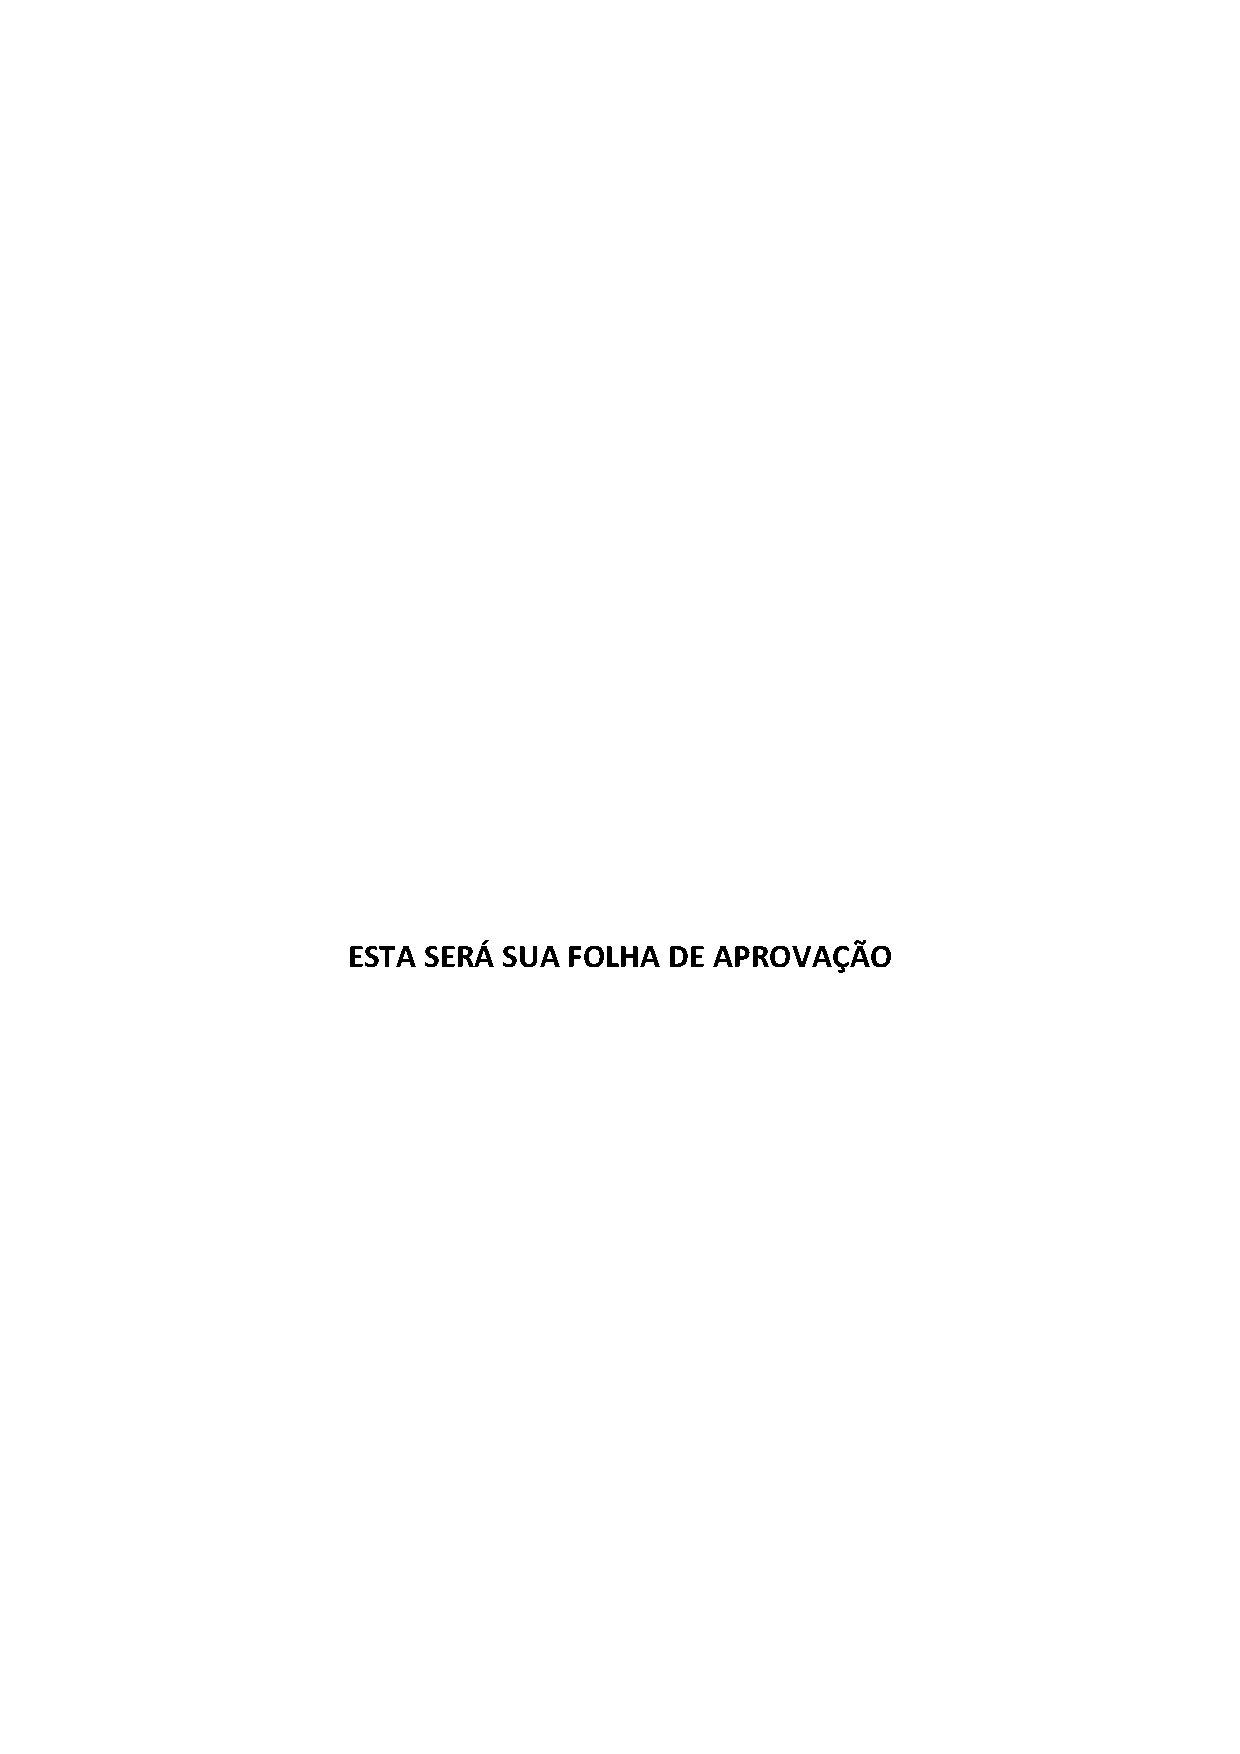
\includepdf[pages=-]{anexos/aprovacao.pdf}

\setlength{\ABNTEXsignwidth}{12cm}

%--------------------------------------------------------------------------------
% Está comentado pelo mesmo motivo da ficha catalográfica 
%--------------------------------------------------------------------------------
%\begin{folhadeaprovacao}
%	\begin{center}
%	    {\ABNTEXchapterfont\bfseries\large\imprimirinstituicao}
%	    \vspace*{\fill}
%
%	    {\ABNTEXchapterfont\bfseries\large FOLHA DE APROVAÇÃO}
%	    \vspace*{\fill}
%
%	    {\ABNTEXchapterfont\bfseries\large\imprimirautor}
%
%	    \vspace*{\fill}\vspace*{\fill}
%	    {\ABNTEXchapterfont\bfseries\large\imprimirtitulo}
%	    \vspace*{\fill}
%
%	    {\hspace{.45\textwidth}
%		\begin{minipage}{.5\textwidth}
%			\SingleSpacing
%			\ABNTEXchapterfont\imprimirpreambulo \\ \\
%
%			{\ABNTEXchapterfont\imprimirorientadorRotulo~\imprimirorientador\par}
%			{\ABNTEXchapterfont\imprimircoorientadorRotulo~\imprimircoorientador\par}
%
%		\end{minipage}%
%	    \vspace*{\fill}}
%	\end{center}
%
%	\vspace*{\fill}	
%	
%	\begin{center}
%			 \ABNTEXchapterfont\large Aprovado em: \_\_\_\_ de \_\_\_\_ de 2017
%	\end{center}

%	\vspace*{\fill}
	
%	\begin{center}
%			 \ABNTEXchapterfont\bfseries\large Banca Examinadora
%	\end{center}
%		
%   \ABNTEXchapterfont\assinatura{Fábio Nelson de Sousa Pereira, Mestre, Universidade Federal do Vale do São Francisco}
%	\ABNTEXchapterfont\assinatura{Jorge Luis Cavalcanti Ramos, Doutor, Universidade Federal do vale do São Francisco}
%  \ABNTEXchapterfont\assinatura{Ricardo Argenton Ramos, Doutor, Universidade Federal do Vale do São Francisco}
%	 \vspace*{\fill}

	 
%\end{folhadeaprovacao}

%--------------------------------------------------------------------------------
% Insere a epígrafe
%--------------------------------------------------------------------------------
% \newpage
% \vspace*{\fill}
% \begin{flushright}
% 		\textit{Lorem Ipsum...}
% \end{flushright}

%--------------------------------------------------------------------------------
% Seção de agradecimentos
%--------------------------------------------------------------------------------
% \begin{agradecimentos}
	
% \lipsum[2-4]

% \end{agradecimentos}

%--------------------------------------------------------------------------------
% Insere a segunda epígrafe
%--------------------------------------------------------------------------------
% \begin{epigrafe}
%     \vspace*{\fill}
% 	\begin{flushright}
% 		Se pude enxergar a tão grande distância, foi subindo nos ombros de gigantes.\\
% 		 \vspace{\baselineskip}
% 		\textbf{Isaac Newton}\\
% 		\textbf{Carta à Robert Hooke, 1676}
% 	\end{flushright}
% \end{epigrafe}



%--------------------------------------------------------------------------------
% Seção de resumos
%--------------------------------------------------------------------------------
% resumo em português
\setlength{\absparsep}{18pt} % ajusta o espaçamento dos parágrafos do resumo
\begin{resumo}

Um dos atributos mais significativos para a garantia da qualidade de uma fruta é a quantidade de açúcares nela contida. Entretanto, para a obtenção deste valor, é 
exigida a destruição da amostra, de forma que seu conteúdo seja analisado. Essa abordagem, além de destrutiva, é onerosa; assim, o emprego de um sistema de visão 
computacional para previsão desta variável de saída mostra-se vantajoso. Entretanto, é necessário definir as variáveis visuais da fruta a partir das quais o teor 
de sólidos solúveis será obtido. Assim, foi conduzido um estudo baseado em diferentes artigos onde é empregado o processamento de imagens para predição de atributos
 de qualidade. A fruta analisada foi a manga, da variedade ‘Palmer’, por ser produzida em abundância no Vale do São Francisco e por contribuir para a economia de 
 Juazeiro (BA) e Petrolina (PE) através de sua exportação. As melhores técnicas de pré-processamento e inferência também foram avaliadas, de forma a obter a melhor 
 abordagem para predição de sólidos solúveis em manga. Foi encontrado que as melhores técnicas de pré-processamento foram filtro da mediana, operações de abertura e fechamento e limiarização simples. Os atributos visuais mais significantes foram a dimensão de correlação, taxa R/B e as médias do canal B na região equatorial e da haste. O coeficiente de correlação foi igual a 0,9752, obtido através da \textit{Random Forest}.

 \textbf{Palavras-chave}: Quantidade de açúcares. Visão computacional. \textit{Random Forest}.

\end{resumo}

%---------------------------------------------------------------------------------
% resumo em inglês
\begin{resumo}[Abstract]
\begin{otherlanguage*}{english}

One of the most significant attributes for guaranteeing the quality of a fruit is the amount of sugars contained in it. However, to obtain this value, the destruction 
of the sample is required, so that its content is analyzed. This approach, besides being destructive, is onerous; thus, the use of a computer vision system to predict 
this output variable is advantageous. However, it’s necessary to define the fruit’s visual variables from which the sugar content will be obtained. Thus, the study 
was conducted based on different articles in which image processing is employed to predict quality attributes. The analyzed fruit was the mango, from ‘Palmer’
 variety, due to its abundant production in the São Francisco Valley and its contribution to the economy in Juazeiro (BA) and Petrolina (PE) through exportation. 
 The best pre-processing and inference techniques were also evaluated in order to obtain the best approach to predict sugars in mangoes. It was found that the best pre-processing techniques were median filter, opening and closing operations and thresholding. The most significant visual aspects were the correlation dimension, R/B rate and the B channel mean in the stalk and apex regions. The correlation coefficient was equal to 0,9752 and was obtained through Random Forest.

	\vspace{\onelineskip}

	\noindent
	\textbf{Key-words}: \textit{Sugar content. Computer vision. Random Forest}.

\end{otherlanguage*}
\end{resumo}


%---------------------------------------------------------------------------------
% Insere lista de ilustrações
%---------------------------------------------------------------------------------
\begin{KeepFromToc} % Este comando evita que todas as seções dentro dele de apareçam no sumário
\pdfbookmark[0]{\listfigurename}{lof}
\listoffigures
%\addcontentsline{toc}{chapter}{Lista de Figuras}
\cleardoublepage


%---------------------------------------------------------------------------------
% Insere lista de tabelas
%---------------------------------------------------------------------------------
\pdfbookmark[0]{\listtablename}{lot}
\listoftables
\cleardoublepage

%---------------------------------------------------------------------------------
% Ajusta lista de código - alterar de figures para códigos - by @Gabrielr2508
%---------------------------------------------------------------------------------
% \makeatletter
% \let\l@listing\l@figure
% \def\newfloat@listoflisting@hook{\let\figurename\listingname}
% \makeatother

%---------------------------------------------------------------------------------
% Insere lista de códigos - by @leolleocomp
%---------------------------------------------------------------------------------
% \listoflistings

\end{KeepFromToc}

%---------------------------------------------------------------------------------
% Insere lista de abreviaturas e siglas
%---------------------------------------------------------------------------------
\begin{siglas}
	\item[BCD]		Dimensão de contagem de caixa – \textit{Box Counting Dimension}
	\item[CCD]		Dispositivo de carga acoplada – \textit{Charge-coupled Device}
	\item[CD]		Dimensão de correlação – \textit{Correlation Dimension}
	\item[DD]		Dimensão de dilatação – \textit{Dilation Dimension}
	\item[LS-SVM]		Máquina de vetores de suporte por mínimos quadrados – \textit{Least-Squares Support Vector Machine}
	\item[MDA]		Análise discriminante múltipla – \textit{Multiple Discriminant Analysis}
	\item[MLR]		Regressão linear múltipla – \textit{Multiple Linear Regression}
	\item[PCA]		Análise de componentes principais – \textit{Principal Component Analysis}
	\item[RBF]		Função de base radial – \textit{Radial Basis Function}
	\item[RMSE]		Raiz do erro quadrático médio – \textit{Root Mean Square Error}
	\item[RFE]		Eliminação recursiva de atributos - \textit{Recursive Feature Elimination}
	\item[RNA]		Rede neural artificial
	\item[RPI]		\textit{Ripening Index}
	\item[RSS]		Soma do quadrado dos resíduos – \textit{Residual Sum of Squares}
	\item[SST]		Sólidos solúveis totais
	\item[SVM]		Máquina de vetores de suporte – \textit{Support Vector Machine}
	    
\end{siglas}

%---------------------------------------------------------------------------------
% Insere o sumario
%---------------------------------------------------------------------------------
\pdfbookmark[0]{\contentsname}{toc} 
\tableofcontents*
\cleardoublepage


	\textual
		\pagestyle{simple}
		%--------------------------------------------------------------------------------------
% Este arquivo contém a sua introdução, objetivos e organização do trabalho
%--------------------------------------------------------------------------------------
\chapter{Introdução}

O Nordeste é uma das regiões de destaque na produção de manga, particularmente nas áreas irrigadas do semiárido, que apresentam boas condições para o desenvolvimento desta fruta (EMBRAPA SEMIÁRIDO, 2010). Em 2015, a região foi responsável por 70\% das áreas colhidas, na qual a Bahia e Pernambuco foram os maiores contribuidores, alcançando as duas primeiras colocações na produção de manga dentre os demais estados (ANUÁRIO BRASILEIRO DE FRUTICULTURA, 2017). Na Bahia e Pernambuco, destacam-se as cidades de Juazeiro (BA) e Petrolina (PE), localizadas no Vale do São Francisco. No ano de 2016, elas foram responsáveis por quase 30\% da produção nacional (PAM, 2017) e por 89\% da exportação de manga no ano de 2014 (BRANCO, 2016).

Para a manutenção da demanda por mangas do Vale do São Francisco, é necessário prezar pela qualidade do produto, sendo este um fator crucial considerado pelo consumidor no momento da compra. Dentre os atributos determinantes para a qualidade da manga, destaca-se sua doçura (SANTOS NETO et al., 2017). Este atributo é representado pelos sólidos solúveis totais (SST), que representam o conteúdo total de açúcares na fruta (SCHMUTZLER; HUCK, 2016). Entretanto, este atributo é normalmente obtido através de um refratômetro\footnote{\label{ftnote:refratometer}Instrumento óptico utilizado para determinar o índice de refração de uma substância (FERRAZ, 2015). Ele pode ser utilizado para monitorar a concentração de açúcar em uma solução, retornando um valor em ºBrix, que corresponde a um grama de açúcar (sacarose) por 100g da solução.}, que quantifica os SST contido no suco extraído, o que exige a destruição das amostras no processo, impossibilitando a comercialização das mesmas. Assim, surge a necessidade de determinar este atributo através de uma metodologia que não destrua as amostras.

Neste contexto, destaca-se a visão computacional, subárea da Inteligência Artificial que dá aos computadores a capacidade de aprendizado e inferência com base em informações visuais (GONZALEZ; WOODS, 2009). Em um sistema desse tipo as imagens digitais são manipuladas através de processamento de imagens, visando a extração de informações significativas sobre as mesmas. Assim, o teor de SST em mangas pode ser obtido a partir das fotos tiradas das frutas, através de um modelo preditivo que relacione este teor com as informações visuais extraídas da manga. Um sistema de visão computacional, além de eliminar a necessidade da destruição das amostras, pode possibilitar a determinação do atributo desejado de forma rápida e precisa.

\section{Motivação}

O trabalho proposto possui potencial para beneficiar a comercialização da manga ao viabilizar a automatização de processos manuais. Assim, a determinação da qualidade das frutas torna-se mais rápida, econômica e consistente (DONIS-GONZÁLEZ et al., 2013). Como a obtenção do teor de sólidos solúveis não exige a destruição das amostras, produtoras \textcolor{red}{e/ou consumidores} de mangas não teriam mais o prejuízo do descarte, além de poderem proporcionar ao mercado consumidor um produto com qualidade assegurada. 

\section{Definição do Problema}

Para a obtenção de uma informação desejada a partir de uma imagem, é necessário cumprir uma sequência de etapas que se inicia na aquisição das imagens das amostras. Segundo Esquef (2002), após a aquisição é realizado o pré-processamento das imagens. Esta etapa é fundamental em um sistema de visão computacional, sendo necessária para remover informações indesejadas, realçar ou atenuar algumas das partes da imagem. Após ser realizado o pré-processamento, é aplicada a segmentação, para que a imagem seja dividida em partes disjuntas, visando sua simplificação (JOSEPH; SINGH, 2014). No contexto deste trabalho, a única região de interesse é a manga; assim, as imagens foram segmentadas visando a separação entre a fruta e o plano de fundo. A penúltima etapa realizada foi a extração de atributos, em que para cada imagem é obtido um conjunto de características que a define. Por fim, estes atributos de cada imagem foram relacionados ao atributo desejado através de um modelo preditivo.

Entretanto, a escolha de técnicas de pré-processamento de imagens e atributos empregados não é realizada de forma trivial e depende da natureza do problema. Logo, para a construção de um bom modelo preditivo de sólidos solúveis totais (SST), diferentes técnicas de pré-processamento foram testadas e, para a determinação dos atributos mais significativos, um estudo investigativo sobre elas foi conduzido. Por fim, a relação entre os atributos e o SST deverá ser modelada através de uma Regressão linear e Random Forest, cujos desempenhos foram avaliados através de métricas apropriadas. Assim, através deste estudo se buscou um profundo entendimento entre os aspectos visuais da manga e sua doçura. 

\section{Objetivos}

\subsection{Objetivo Geral}
O objetivo geral do trabalho consiste na identificação de quais atributos de uma imagem da manga devem ser considerados para a predição dos sólidos solúveis. 

\subsection{Objetivos específicos}

\begin{itemize}
	\item Determinar as técnicas de pré-processamento de imagens mais adequadas para o problema;
    \item Realizar um estudo investigativo quanto aos atributos através de modelos de Regressão linear e Random Forest;
    \item \textcolor{red}{Correlacionar as imagens com os atributos físico-químicos das mangas.}
\end{itemize}

\section{Organização do trabalho}

O trabalho possui, além da Introdução, os capítulos de Fundamentação teórica, Materiais e métodos, Resultados e Conclusão. Na fundamentação é discorrido sobre todos os tópicos necessários para o entendimento do trabalho e os artigos selecionados para o estudo. No capítulo de materiais e métodos, é explicada a metodologia a ser aplicada, desde a coleta das mangas até a construção dos modelos preditivos. Os resultados obtidos no trabalho são mostrados no capítulo seguinte e, por fim, no último capítulo é feita uma conclusão sobre o estudo conduzido, assim como potenciais trabalhos futuros.

		%--------------------------------------------------------------------------------------
% Este arquivo contém a sua funtamentação teórica
%--------------------------------------------------------------------------------------
\chapter{Fundamentação teórica}

\section{\textit{Background}}

Para um entendimento apropriado do estudo investigativo, são discutidos aqui conceitos básicos do processamento digital de imagens, como espaços de cores, pré-processamento e técnicas de inferência para determinação de um atributo desejado. 

\subsection{Espaços de cores}

Um espaço de cores é um modelo matemático utilizado para a representação de uma cor através de três ou mais componentes (SHAIK et al., 2015). Um espaço de cor pode ser orientado a um hardware específico, como o modelo RGB (\textit{Red, Green, Blue}), para exibição em monitores coloridos ou aquisição por uma câmera digital. Entretanto, este espaço de cor não permite uma interpretação humana exata de como a cor é composta. Por outro lado, espaços de cores como o L*a*b* e HSV (\textit{Hue}, \textit{Saturation}, \textit{Value}) permitem uma descrição mais natural. 

\subsubsection{RGB}

Este modelo é baseado nas três cores primárias, a partir das quais ele é nomeado: vermelho (\textit{Red}), verde (\textit{Green}) e azul (\textit{Blue}). Ele é representado por um sistema de coordenadas 3D, em que cada cor é dada por um vetor que se origina na origem. Os três elementos do vetor consistem nas intensidades de cada cor primária, e assim, uma imagem RGB é representada por três matrizes, cada uma contendo as intensidades do respectivo canal (R, G, B) para todos os pixels da imagem. Quando as três cores são combinadas em suas intensidades máximas, o olho humano percebe a cor resultante como branca. Por outro lado, quando as três intensidades são nulas, tem-se a cor preta como resultante. No subespaço RGB, mostrado na Figura \ref{img:rgb_cube}, o segmento de reta que une as cores branca e preta consiste na escala de cinza, onde as intensidades dos três canais são iguais. Os demais vértices do cubo correspondem às cores primárias e secundárias (SONKA; HLAVAC; BOYLE, 2014).  

\begin{figure}[H]
\centering
    \caption{\label{img:rgb_cube} Subespaço de cores RGB.}
    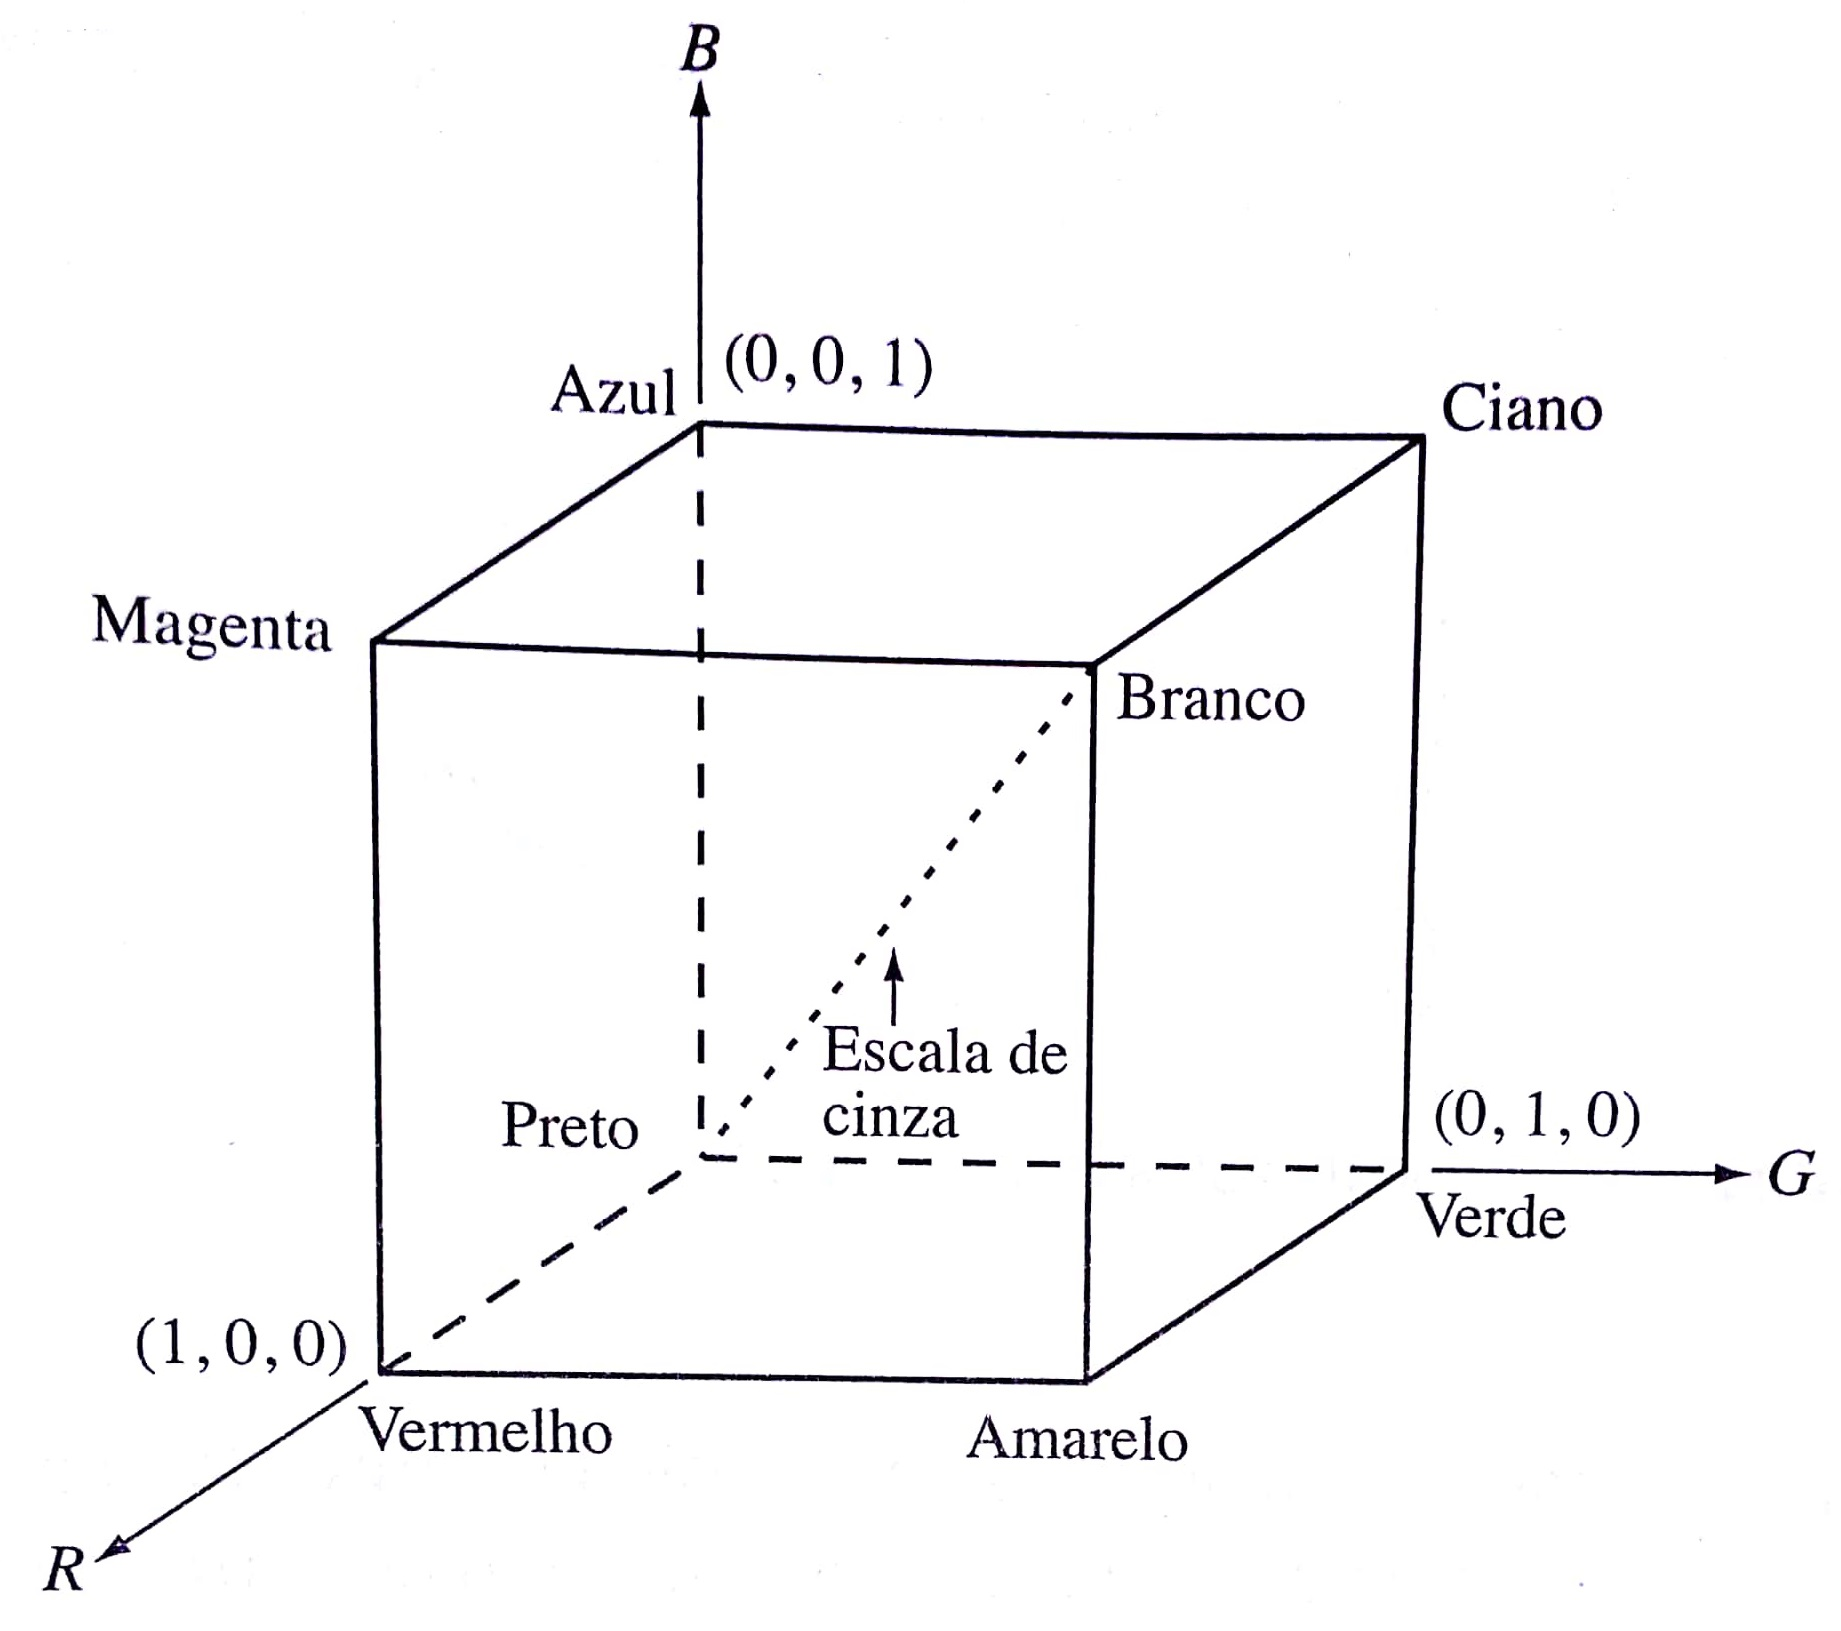
\includegraphics[scale=0.09]{img/rgb_cube}
    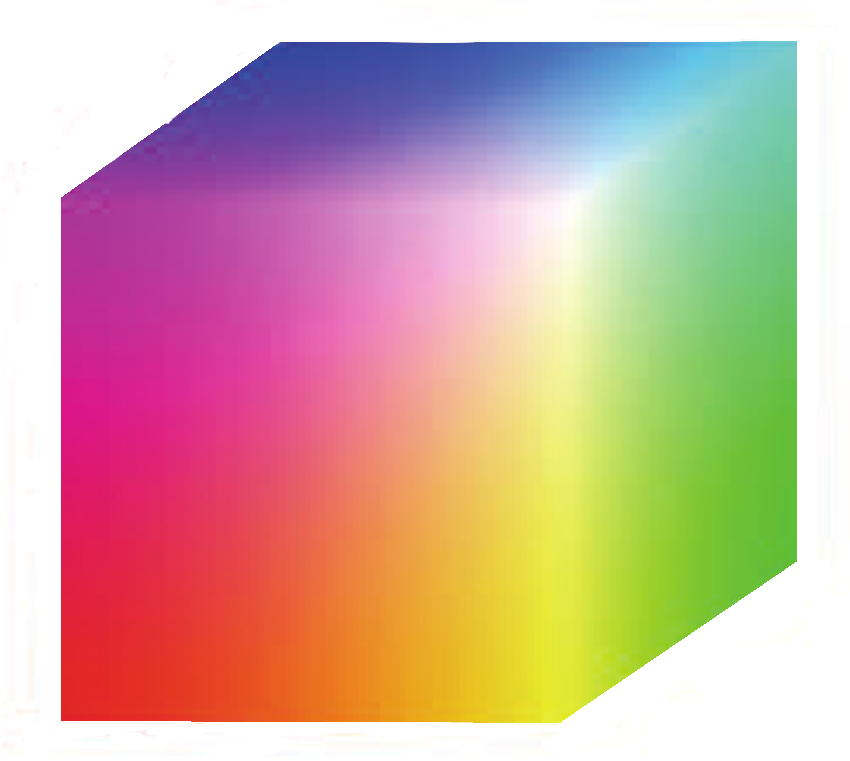
\includegraphics[scale=0.15]{img/rgb_cube2}
    \legend{\textbf{Fonte: } (GONZALEZ; WOODS, 2009; DATAR; JONES; SMITH JR., 2005).}
\end{figure}

\subsubsection{L*a*b*}

Este espaço de cores, também chamado de CIE-Lab, emprega como componentes a luminosidade (L*), que varia entre 0 (preto)  e 100 (branco) e os canais “vermelho-verde” (a*) e “amarelo-azul” (b*). Estes últimos canais representam a variação da cor entre verde até vermelho e amarelo até azul respectivamente. A representação de uma imagem neste sistema de cores é obtida a partir da conversão do espaço RGB para o XYZ inicialmente, através da equação (\ref{eq:xyz}):

\begin{equation} \label{eq:xyz}
	\begin{bmatrix}
		X \\
		Y \\
		Z \\
	\end{bmatrix} =
	\begin{bmatrix}
		0,4125 & 0,3576 & 0,1804 \\
		0,2127 & 0,7152 & 0,0722 \\
		0,0193 & 0,1192 & 0,9502
	\end{bmatrix}
	\begin{bmatrix}
		R \\
		G \\
		B \\
	\end{bmatrix}
\end{equation}

Após essa conversão, os valores L*, a* e b* são obtidos a partir das equações (\ref{eq:lab1}), (\ref{eq:lab2}) e (\ref{eq:lab3}) (KAUR; KRANTHI, 2012), em que ($X_b$,  $Y_b$,  $Z_b$) é a coordenada que representa a cor branca neste espaço de cor.  

\begin{equation} \label{eq:lab1}
	L* =
		\begin{cases}
			116*(\frac{Y}{Y_b})^{\frac{1}{3}} - 16 & onde \ \frac{Y}{Y_b} > 0,008856 \\
			903,3 									& onde \ \frac{Y}{Y_b} \leq 0,008856
		\end{cases}
\end{equation}

\begin{equation} \label{eq:lab2}
	a* = 500 * 
		\begin{bmatrix}
			\frac{X^\frac{1}{3}}{X_b} - \frac{Y^\frac{1}{3}}{Y_b}
		\end{bmatrix}
\end{equation}

\begin{equation} \label{eq:lab3}
	b* = 200 *
		\begin{bmatrix}
			\frac{X^\frac{1}{3}}{X_b} - \frac{Z^\frac{1}{3}}{Z_b}
		\end{bmatrix}
\end{equation}

\subsubsection{HSV}

O sistema HSV, também conhecido como HSB, possui como componentes a matiz (\textit{Hue}), saturação (\textit{Saturation}) e valor ou brilho (\textit{Value} ou \textit{Brightness}), sendo capaz de descrever uma cor de uma forma mais intuitiva para os humanos (NADAFZADEH; MEHDIZADEH; SOLTANIKAZEMI, 2018).

A matiz é associada à cor dominante em uma mistura de cores, da forma como é percebida por um humano. Ela é descrita em graus, variando entre 0º e 360º, de acordo com sua localização na roda de cores, conforme a Figura \ref{img:hsv_hex}. A saturação mede o grau de diluição de uma cor pura por luz branca, sendo estimada de acordo com a distância da cor até a origem do cone, que representa a cor branca. Por fim, o valor ou brilho indica a quantidade de luz na combinação, sendo obtida a partir da distância da cor a partir do preto até o branco. Tanto a saturação quanto o valor/brilho possuem valores variando entre 0 e 1 (DORJ; LEE; YUN, 2017).

\begin{figure}[H]
\centering
    \caption{\label{img:hsv_hex} Representação 3D do espaço de cores HSV.}
    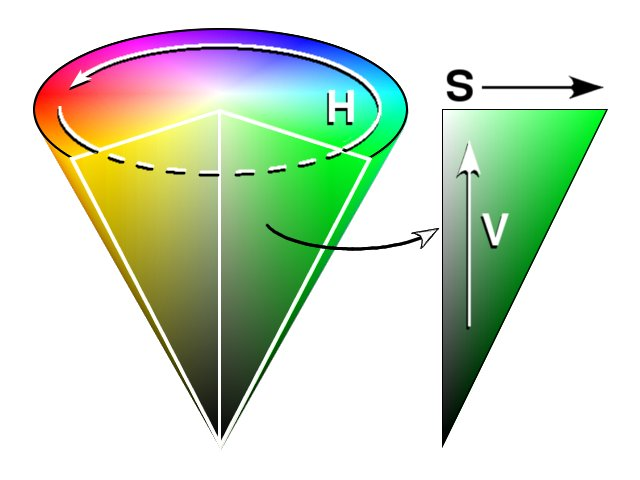
\includegraphics[scale=0.25]{img/hsv_hex}
    \legend{\textbf{Fonte: } (Wikipedia, 2019).}
\end{figure}

Pode ser realizada a conversão de uma imagem no espaço de cores RGB para HSV, de forma a se obter uma melhor descrição da mesma, através das seguintes equações: 

\begin{equation} \label{eq:hsv1}
	H = \begin{cases}
			\theta, 		& se \ B \leq G \\
			360 - \theta, 	& se \ B > G
		\end{cases}
\end{equation}

\begin{equation} \label{eq:hsv2}
	\theta = \arccos{
		\Bigg\{ \frac{\frac{1}{2}[(R - G) + (R - B)]}{\sqrt{[(R - G)^2 + (R - G)*(G - B)]}}
	}
\end{equation}

\begin{equation} \label{eq:hsv3}
	S = 1 - \frac{3}{R + G + B}[mín(R,G,B)]
\end{equation}

\begin{equation} \label{eq:hsv4}
	V = \frac{1}{3}(R + G + B)
\end{equation}

\subsection{Pré-processamento de imagens}

A seguir estão descritas algumas das técnicas de pré-processamento mais comuns. Elas subdividem-se quanto ao domínio em que atuam, podendo ser realizadas no domínio espacial, em que as técnicas são aplicadas nos pixels diretamente, ou no domínio da frequência, em que os métodos são realizados no espectro de frequência da imagem (BEDI; KHANDELWAL, 2013). 

\subsubsection{Filtro da mediana}

A filtragem da mediana consiste em uma operação não linear realizada no domínio espacial. Através dela o ruído de uma imagem é removido enquanto as bordas são preservadas, pois ele não é tão sensível a valores extremos. Para realizar a filtragem, move-se uma janela de tamanho predefinido pixel a pixel, de forma que cada valor seja substituído pela mediana dos valores dos pixels contidos na janela (HEMALATHA; SUMATHI, 2016). Este filtro é comumente empregado para imagens com ruído do tipo \textit{salt and pepper}, que consiste em pixels aleatórios de cor branca ou preta, conforme mostra a Figura \ref{img:median_filter}.

\imagem{0.5}{median_filter}{Remoção de ruído \textit{salt and pepper} por um filtro da mediana com tamanho da janela igual a 3x3.}{(MathWorks Inc., 2006).}

\subsubsection{Operações de abertura e fechamento (\textit{Opening and closing operations})}

As operações de abertura e fechamento são do tipo morfológicas, em que são realizadas transformações em uma imagem, normalmente binária, com base no formato do objeto nela contido. Elas se diferem quanto à ordem em que as operações de erosão e dilatação, também morfológicas, são realizadas em uma imagem.

Nestas duas operações, um \textit{kernel}, que consiste em uma janela de tamanho predefinido preenchida com 0s ou 1s, percorre a imagem original, substituindo o valor de um pixel caso os pixels contidos na janela sejam todos iguais a 1, no caso da erosão, ou pelo menos um deles seja igual a 1, no caso da dilatação. Na Figura \ref{img:eros_dilat} são mostrados os efeitos do uso da erosão e dilatação em uma mesma imagem.

\begin{figure}[H]
\centering
    \caption{\label{img:eros_dilat} Utilização da erosão e dilatação em uma imagem (a) Imagem original (b) Imagem erodida (c) Imagem dilatada.}
    \subcaptionbox{}{
\includegraphics[scale=0.6]{img/j.png}}
    \subcaptionbox{}{
\includegraphics[scale=0.6]{img/j_eros.png}}
    \subcaptionbox{}{
\includegraphics[scale=0.6]{img/j_dilat.png}}
    \legend{\textbf{Fonte: } (OpenCV, 2019).}
\end{figure}

A operação de abertura realiza a erosão seguida de dilatação, resultando na eliminação de ruídos pontuais enquanto mantém as formas do objeto. Por outro lado, a operação de fechamento primeiro aplica a dilatação e depois a erosão, o que, além de também manter o contorno do objeto, contribui para o preenchimento de pequenos buracos (ARCO et al; 2015). A Figura \ref{img:morph_op} mostra o resultado da utilização destas operações. 

\begin{figure}[H]
\centering
    \caption{\label{img:morph_op} Operações morfológicas aplciadas na letra "j" (a) Abertura (b) Fechamento.}
    \subcaptionbox{}{
\includegraphics[scale=0.6]{img/opening.png}}
    \subcaptionbox{}{
\includegraphics[scale=0.6]{img/closing.png}}
    \legend{\textbf{Fonte: } (OpenCV, 2019).}
\end{figure}

\subsection{Segmentação de imagens}

O objetivo da segmentação consiste em dividir a imagem em subconjuntos disjuntos, de forma a obter apenas a região desejada. A segmentação torna-se simples quando na imagem em questão há objetos contrastantes em um fundo uniforme. Dessa forma, pode-se utilizar uma abordagem baseada no histograma da imagem, que fornece a frequência dos níveis de intensidade dela (GONZALEZ; WOODS, 2009).

\subsubsection{Limiarização}

A limiarização é o método de segmentação mais simples, rápido e pouco custoso existente. Ela é utilizada em imagens em que os objetos nela presentes possuem uma absorção de luz uniforme ao longo de suas superfícies, de forma que, a partir de um valor limiar, ou \textit{threshold}, é possível fazer a separação completa dos objetos da imagem (SONKA; HLAVAC; BOYLE, 2008).

Assim, dada uma imagem $f(i, j)$, obtém-se uma imagem segmentada $g(i, j)$ conforme a equação abaixo, considerando um \textit{threshold} T dado:

\begin{equation} \label{eq:thrd}
	g(i, j) =
		\begin{cases}
			1, & se \ f(i, j) \geq T, \\	
			0, & se \ f(i, j) < T
		\end{cases}
\end{equation}

Na Figura \ref{img:thresholding} é mostrado o resultado da limiarização simples aplicada numa imagem gradiente em escala de cinza. Como esta imagem é representada em 8 bits e seus valores de intensidade  variam entre 0 e 255 ($2^8$), ao utilizar um limiar igual a 127, a imagem resultante consiste em duas metades cujos pixels são iguais a 0 e 1. 

\begin{figure}[H]
\centering
    \caption{\label{img:thresholding} Limiarização simples aplicada em uma imagem, com \textit{threshold} igual a 127. À esquerda, a imagem gradiente, cuja intensidade varia entre 0 e 255. À direita, o resultado da limiarização.}
    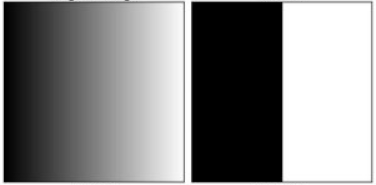
\includegraphics[scale=0.5]{img/thresholding.png}
    \legend{\textbf{Fonte: } (OpenCV, 2003).}
\end{figure}

\subsubsection{Segmentação de Otsu}

Esta técnica de segmentação é eficaz para imagens bimodais, cujos histogramas possuem dois picos. Este método calcula um limiar ótimo que se localiza aproximadamente no meio dos dois picos (GONZALEZ; WOODS, 2009). O algoritmo de Otsu busca um \textit{threshold} t tal que a variância entre uma mesma classe é minimizada. No contexto de uma imagem, uma classe seria o objeto de estudo ou o plano de fundo. A função a ser minimizada é dada por:

\begin{equation} \label{eq:otsu}
	\sigma_w^2(t) = q_1(t)\sigma_1^2(t) + q_2(t)\sigma_2^2(t)
\end{equation}

Em que $q_1(t)$ e $q_2(t)$ são as probabilidades das classes associadas ao limiar t, dadas por:

\begin{equation}
	q_1(t) = \sum_{i=1}^t{P(i)} \;\;\;\;\;\; q_2(t) = \sum_{i=t+1}^I{P(i)}
\end{equation}

Em que $P(i)$ é o histograma da imagem, tratado como função de densidade de probabilidade, e I é o nível máximo de intensidade da imagem. $\sigma_1^2(t)$ e $\sigma_2^2(t)$ são as variâncias das classes, dadas por:

\begin{equation}
	\sigma_1^2(t) = \sum_{i=1}^t{[i-\mu_1(t)]^2\frac{P(i)}{q_i(t)}} \;\;\;\; \sigma_2^2(t) = \sum_{i=t+1}^I{[i-\mu_1(t)]^2\frac{P(i)}{q_2(t)}}
\end{equation}

Em que:

\begin{equation}
	\mu_1(t) = \sum_{i=1}^t{i\frac{P(i)}{q_i(t)}} \;\;\;\; \mu_2(t) = \sum_{i=t+1}^I{i\frac{P(i)}{q_2(t)}}
\end{equation}

Na Figura \ref{fig:otsu} é mostrada uma imagem original e o resultado da segmentação de Otsu.

\begin{figure}[H]
\centering
    \caption{\label{fig:otsu} Segmentação de Otsu. À esquerda, a imagem original. À direita, a imagem segmentada pelo algoritmo de Otsu}
    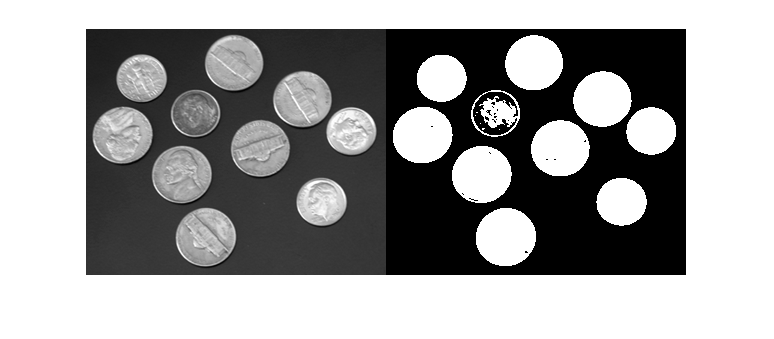
\includegraphics[scale=0.5]{img/otsu.png}
    \legend{\textbf{Fonte: } (Mathworks Inc., 2006).}
\end{figure}

\subsection{Técnicas de inferência}

As técnicas aqui apresentadas são empregadas para a predição de uma variável de saída desejada com base nas variáveis de entrada fornecidas, através de modelos supervisionados de regressão ou classificação, em que a variável de saída é quantitativa ou qualitativa, respectivamente (DA SILVA; PERES; BOSCARIOLI, 2017). Para tal, deve-se utilizar um conjunto de amostras de treinamento, em que as variáveis de entrada e saída são conhecidas, para a construção de um modelo matemático que extraia padrões a partir dos dados fornecidos. Assim, tendo modelado o relacionamento entre as variáveis, pode-se realizar a predição para novas amostras, em que sua variável de saída é desconhecida (GAMA, 2015).

\subsubsection{Regressão linear múltipla}

A MLR (\textit{Multiple Linear Regression}) é um método de regressão que assume um relacionamento linear entre os atributos de entrada e o de saída (JAMES et al., 2013). Ela é uma extensão da regressão simples, que emprega apenas uma variável de entrada, e apresenta um bom desempenho quando empregada em um conjunto de dados que não possua ruído ou colinearidade entre os atributos. A equação que descreve a MLR é dada por:

\begin{equation} \label{eq:mlr}
	Y = \beta_0 + \beta_1 X + \epsilon
\end{equation}

Em que $Y$ é o vetor de atributo alvo, $\beta_0$ é o intercepto, $\beta_1$ é o vetor de inclinações da equação, $X$ é o vetor de atributos e $\epsilon$ é o erro aleatório. 

Os parâmetros da MLR são normalmente estimados pelo método dos mínimos quadrados, que busca minimizar a soma do quadrado dos resíduos (RSS – \textit{Residual Sum of Squares}), dada pela equação abaixo:

\begin{equation} \label{eq:rss}
	RSS = e_1^2 + e_2^2 + ... + e_n^2
\end{equation}

Em que $e_1^2$, $e_2^2$, ..., $e_n^2$ correspondem à diferença entre o valor previsto pelo modelo e o valor real para as $n$ amostras. 

\subsubsection{\textit{Random Forest}}

A \textit{Random Forest} consiste em uma técnica \textit{ensemble} não linear, em que uma variável qualitativa ou quantitativa é determinada através de uma combinação de modelos de árvores de decisão (FRIEDMAN; HASTIE; TIBSHIRANI, 2001). A relação entre as variáveis de entrada e a de saída é modelada através de um conjunto de regras de decisão, construídas por divisões binárias e recursivas dos dados de treinamento. Cada regra de decisão utiliza uma única variável de entrada para a divisão dos dados, sendo ela selecionada a partir de um subconjunto aleatório de todas as variáveis. Um modelo de regressão é então construído a partir das variáveis selecionadas e o erro RSS é calculado (HUTENGS; VOHLAND, 2016). As regras de decisão e consequentemente as variáveis de entrada, são selecionadas visando a minimização desse erro. Assim, a \textit{Random Forest} permite a determinação das variáveis mais significativas para a predição da variável de saída. 

O valor previsto resultante será a média dos resultados obtidos para cada árvore de decisão. Para evitar a correlação entre as árvores, elas são construídas a partir de subconjuntos não disjuntos dos dados de entrada, o que torna o modelo resultante mais estável, robusto e preciso (BREIMAN, 2001).

\subsection{Avaliação do desempenho de modelos}

Para a avaliação da capacidade preditiva dos modelos, é comumente utilizada a estratégia de validação cruzada k-\textit{fold} (k-\textit{fold cross validation}). Ela é empregada para assegurar que não há um sobreajuste (\textit{overfitting}) no modelo, através da divisão do conjunto de dados em k subconjuntos disjuntos, com uma alocação das amostras para o conjunto de treinamento ou teste (DA SILVA; PERES; BOSCARIOLI, 2017). Assim, um dos subconjuntos é utilizado como teste e os k-1 demais para o treinamento, de forma que o modelo realize a predição para dados desconhecidos. Este procedimento é repetido k vezes, alterando os subconjuntos a cada vez.

As predições resultantes podem então ser avaliadas através de métricas, tais como o coeficiente de correlação e RMSE, empregadas nos artigos em que a regressão foi realizada. Estes indicadores medem, respectivamente, o grau de dependência entre as variáveis de entrada e saída e a magnitude média dos erros estimados (ALVES; VECCHIA, 2011), conforme as equações abaixo:

\begin{equation} \label{eq:r}
	R = \frac{\sum_{i=1}^n (x_i - \overline{x})(y_i - \overline{y})}{\sqrt{\sum_{i=1}^n(x_i - \overline{x})^2} \sqrt{\sum_{i=1}^n (y_i - \overline{y})^2}}
\end{equation}

\begin{equation} \label{eq:rmse}
	RMSE = \sqrt{\frac{1}{n} \sum_{i=1}^n (y_i - \hat{y}_i)^2}
\end{equation}

Em que $x_i$ é o valor da variável de entrada, $\overline{x}$ é a média dos valores de $x$, $y_i$ é o valor real da variável de saída, $\overline{y}$ é a média dos valores de $y$, $n$ é o número de amostras e $\hat{y}_i$ é o valor previsto para a variável de saída.

\section{Trabalhos relacionados}

A seguir são discutidos dez artigos \textit{(Apêndice A)} em que é empregado o processamento digital de imagens para determinação de atributos de qualidade em mangas. O estudo investigativo foi conduzido de acordo com as técnicas e métricas empregadas pelos autores, assim como os atributos extraídos das imagens das mangas. 

Teoh e Syaifudin (2007) propuseram em seu trabalho a determinação do peso de mangas da variedade Chokanan\footnote{\label{ftnote:chokanan}Variedade originária da Tailândia, caracterizada por frutos compridos com pontas cônicas, polpa sem fibra, pele grossa e alta resistência a doenças.} através de imagens obtidas por uma câmera digital. 100 amostras aleatórias de mangas maduras e verdes foram coletadas e divididas entre treinamento e teste (50 para cada conjunto). Os valores reais do peso das mangas foram obtidos por uma balança digital. As mangas foram inicialmente imersas em água e limpas usando uma esponja e, após isso, foram postas em uma superfície preta e tiveram suas imagens tiradas por uma câmera de 0.3m mm/pixel de resolução, que foi situada a 22 cm acima do fruto, com uma fonte de luz de cada lado do aparelho. 

Para o pré-processamento das imagens, inicialmente empregou-se o filtro da mediana de tamanho 15x15 para correção de inconsistências nas imagens devido à iluminação não uniforme. As imagens foram então segmentadas por limiarização, através da análise do histograma bimodal. A Figura \ref{img:img_art_1} mostra os resultados das etapas empregadas pelos autores. A partir da imagem binária foi contado o número de pixels da região da manga, de forma que através desta variável independente o peso da respectiva manga fosse determinado. Um modelo de regressão linear foi então construído utilizando para tal 50 amostras de manga, enquanto que as demais foram empregadas para o teste do modelo, por intervalos de confiança a 95\%. A abordagem proposta pelos autores mostrou-se precisa, alcançando um coeficiente de correlação igual a 97,69\% e erro médio igual a 3,76\%. 

\begin{figure}[!htb]
\centering
    \caption{\label{img:img_art_1} Etapas empregadas pelos autores.}
    \subcaptionbox{Imagem original}{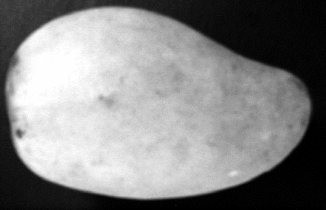
\includegraphics[scale=0.38]{img/art11}}
    \subcaptionbox{Imagem filtrada}{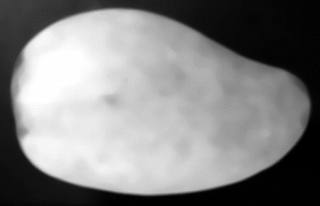
\includegraphics[scale=0.39]{img/art12}}
    \subcaptionbox{Imagem segmentada}{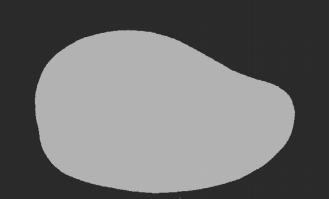
\includegraphics[scale=0.4]{img/art13}}
    \legend{\textbf{Fonte: } (TEOH; SYAIFUDIN, 2007).}
\end{figure}

No estudo de Nandi, Tudu e Koley (2014), mangas de diferentes variedades foram separadas quanto aos dias restantes até o apodrecimento das mesmas. Foram obtidas 1350 amostras de cinco diferentes variedades e provenientes de três pomares, coletadas em três lotes com um intervalo de uma semana entre eles, sendo que em cada lote havia 90 mangas de cada variedade. As mangas foram utilizadas como entrada no sistema automatizado até o dia do apodrecimento delas, resultando em 16400 imagens. Em cada dia, três especialistas determinaram os dias restantes até a data de expiração. As imagens tiradas foram divididas em quatro grupos quanto aos dias restantes até que a respectiva manga apodrecesse (12 dias restantes, 9 até 12 dias, 5 até 8 dias e 1 até 4 dias).

Para a classificação automática das mangas, foi desenvolvido um sistema composto por uma correia transportadora, motor, válvulas solenoides, controladora lógica, câmara de aquisição de imagens e um computador. Uma câmera com Dispositivo de Carga Acoplada (CCD, \textit{Charge-coupled Device}) com resolução 640x480 e frame rate igual a 30 \textit{frames}/s foi posicionada no interior da câmara, iluminada artificialmente, sendo que as imagens foram enviadas ao computador pela porta USB. As mangas eram dispostas na correia transportadora, de forma que, através de válvulas solenoides, elas fossem posicionadas no recipiente relativo à classe prevista. 

Inicialmente os frames adequados foram pré-processados por um filtro \textit{deblurring} de Wiener e filtro da mediana. Após isso, foram convertidos para uma imagem binária e as bordas foram traçadas por um algoritmo baseado em código em cadeia. As imagens das mangas foram então alinhadas em posição vertical para a posterior extração dos atributos. Os autores utilizaram apenas o espaço RGB para tal, levando em consideração o processo de maturação da manga e seu efeito nas regiões da fruta. Assim, as variáveis escolhidas foram as médias dos valores R, G e B da manga inteira e das três regiões (cume, equatorial e haste ou \textit{apex}, \textit{equator} e \textit{stalk}), o gradiente dos três canais ao longo do eixo longitudinal, diferença das médias R, G e B da manga inteira e das três regiões. A Figura \ref{img:art2} exibe as regiões da manga consideradas para a extração de atributos.

\imagem{0.5}{art2}{Imagem pré-processada e segmentada de uma manga, com suas regiões marcadas.}{(NANDI; TUDU; KOLEY, 2014).}

O melhor subconjunto de variáveis foi obtido por eliminação recursiva de atributo (RFE) aliada à SVM, onde se obteve um \textit{ranking} para cada variável. A SVM foi computada iterativamente, incrementando uma variável por vez, obtida a partir de uma lista decrescente de \textit{ranking}. A classificação foi realizada por um ensemble de 7 SVMs binárias, em que cada uma realizava a separação de uma combinação diferente de 2 classes. Os parâmetros ótimos das SVMs e o melhor \textit{kernel} foram obtidos por validação cruzada 6-\textit{fold} através de uma busca em \textit{grid}. Após a classificação ser feita, o computador comunica-se com o controlador lógico que ativa a válvula correspondente à classe prevista e controla a velocidade da correia transportadora. 

O sistema proposto pelos autores apresentou resultados satisfatórios, alcançando uma acurácia média igual a 96\% ao empregar a SVM Gaussian RBF, sendo que o subconjunto de variáveis obtido pelo método RFE continha predominantemente atributos derivados do canal R.

Zheng e Lu (2012) propuseram um método para classificação de mangas quanto a seu estágio de escurecimento empregando a LS-SVM. As 90 mangas coletadas de um supermercado possuíam diferentes graus de escurecimento. Elas foram classificadas visualmente por um perito em três diferentes classes: fresca sem escurecimento, escurecimento moderado e escurecimento severo. Foram então tiradas três imagens de cada manga através de uma câmera digital Canon EOS 50 D, sob iluminação solar. Antes da extração dos atributos, cada imagem foi pré-processada através da sua subtração pelo fundo.

Os atributos extraídos foram os valores médios dos canais L*, a*, b*, e as dimensões fractais dos frutos, que consistem em descritores geométricos das imagens. Estas foram calculadas por três diferentes técnicas: dimensão de contagem de caixa (BCD, \textit{Box Counting Dimension}), dimensão de correlação (CD, \textit{Correlation Dimension}) e dimensão de dilatação (DD, \textit{Dilation Dimension}). 

Na técnica BCD, o espaço euclidiano que contém a imagem é dividido em um \textit{grid} de caixas de tamanho r, que, ao ser diminuído progressivamente, resulta em diferentes quantidades de caixas não vazias, dada por $N(r)$. O valor da variável BCD é então dado por:

\begin{equation} \label{eq:bcd}
	BCD = \lim_{r->0}\frac{\log{N(r)}}{\log{(1/r)}}
\end{equation}

De forma semelhante, na variável DD cada pixel da borda da imagem é substituído por um círculo de diâmetro r que aumenta progressivamente, resultando em diferentes valores para o comprimento de borda $L(r)$ de cada círculo. Assim, o valor DD é encontrado através da Equação \ref{eq:dd}.

\begin{equation} \label{eq:dd}
	DD = \lim_{r->0}{\frac{\log{L(r)}}{\log{(1/r)}}}
\end{equation}

Por fim, CD é uma medida de dimensionalidade, calculada através da \ref{eq:cd}:

\begin{equation} \label{eq:cd}
	CD = \lim_{r->0}{\frac{\log{C(r)}}{\log{(1/r)}}}
\end{equation}

Em que $C(r)$ é dada por:

\begin{equation} \label{eq:c}
	C(r) = \lim_{n->\inf}\frac{1}{N^2} \sum_{j=1}^N \sum_{i=j+1}^N \theta (r - \|R_i - R_j\|)
\end{equation}

Em que $r$ é uma distância limiar, $N$ é o número de pontos, $\theta$ é a função de \textit{Heaviside} e $R$ representa os pontos.

Assim, três diferentes modelos LS-SVM foram computados: um que utiliza apenas as variáveis de cor, outro para as variáveis fractais e o terceiro para todas as variáveis. A Figura \ref{img:art3} exibe as etapas realizadas pelos autores, desde o pré-processamento até a construção dos modelos.

\imagem{0.3}{art3}{Pré-processamento das imagens, extração de seus atributos e posterior construção dos modelos LS-SVM.}{(ZHENG; LU, 2012).}

Os parâmetros ótimos da LS-SVM foram obtidos por uma busca em \textit{grid} aliada à validação cruzada \textit{full}. 70\% das amostras foram escolhidas aleatoriamente para o treinamento da LS-SVM e as demais para o teste, resultando em uma acurácia igual a 100\% para o modelo com todas as variáveis. Por outro lado, o modelo que emprega apenas as variáveis L*a*b* e o que utiliza as variáveis fractais obtiveram acurácias iguais a 88,89\% e 85,19\% respectivamente. 

No trabalho de Khairunniza-Bejo e Kamarudin (2011), determinou-se a doçura de mangas Chokanan\footref{ftnote:chokanan} com o emprego do espaço de cores HSB (ou HSV). O lote colhido pelos autores continha mangas em seis diferentes estádios de maturação. Os valores de SST foram obtidos através de um refratômetro digital em um ambiente a 24,6 ºC. As imagens foram tiradas por uma câmera CCD a 40 cm de distância da manga, em uma sala com iluminação apropriada, resultando em 180 imagens tiradas.

O valor médio dos pixels no espaço HSB foi obtido para cada imagem, conforme mostra a Figura \ref{img:art4}. Cada variável foi empregada para um modelo de regressão linear separadamente, de forma que fosse determinado o melhor canal para determinação de SST em mangas Chokanan\footref{ftnote:chokanan}.

\imagem{0.4}{art4}{Extração de atributos realizada pelos autores.}{(KHAIRUNNIZA-BEJO; KAMARUDIN, 2011).}

A faixa de valores de SST foi dividida em três índices (4,0º - 8.0º, 8.0º - 13.0º e 13.0º - 17.0º), de forma que a regressão fosse aplicada em cada faixa separadamente. Ademais, os nove modelos construídos utilizaram 50\% das imagens enquanto que as demais foram empregadas para o teste. 

A melhor variável obtida foi a matiz, que alcançou uma correlação de Pearson igual a -0,92, enquanto que a saturação e brilho alcançaram coeficientes iguais a 0,85 e 0,66 respectivamente. A matiz apresentou também o menor desvio padrão para os três índices (2,73, 6,31 e 2,44), enquanto que o desvio padrão para o brilho indicou que os valores dos pontos eram bastante dispersos (35,15, 18,09 e 22,79 nos índices 1, 2 e 3 respectivamente). O modelo que emprega matiz apresentou os menores valores para erro médio quadrático no índice 2 e 3 (0,22 e 0,03 ºBrix respectivamente) e a maior Raiz do erro quadrático médio (RMSE, \textit{Root Mean Square Error}) para o índice 1 (0,06 ºBrix). Os modelos com saturação apresentaram os maiores RMSE nos índices 1 e 3, enquanto que o modelo com brilho foi superior no índice 1. Como a diferença entre os erros foi pequena, considerou-se que a matiz provou ser a melhor variável para determinação de SST em mangas, devido ao melhor valor de correlação de Pearson. 

Yossy et al. (2017) propôs um sistema de classificação de mangas quanto ao estádio de maturação e tamanho com o emprego de redes neurais. 52 mangas da variedade Gincu\footnote{\label{ftnote:gincu}A variedade Gedong Gincu é uma das mais populares da Indonésia, lugar de onde se originou. Ela possui um tamanho médio, com seu comprimento entre 10 e 12cm, e peso entre 200 e 250g. Além disso, ela tem um formato arredondado, cor alaranjada e sabor adocicado.} foram empregadas para o treinamento do modelo. Elas possuíam dois tamanhos diferentes (grande e pequeno) e dois estádios diferentes (verde e madura), assim, as classes definidas pelos autores foram grande-madura, pequena-madura, grande-verde e grande-pequena. As imagens foram tiradas através de uma \textit{webcam} a 30 cm de distância e armazenadas como JPEG.

Duas abordagens de pré-processamento foram empregadas a partir da imagem RGB: na primeira, o espaço de cores RGB foi convertido para HSV e a as faixas dos valores H, S e V foram determinadas para a etapa posterior de transformação dos pixels em um \textit{array}. Em seguida, foram aplicadas operações de abertura e fechamento visando a eliminação de objetos e buracos pequenos respectivamente. Por fim, a imagem foi redimensionada para 16x16 pixels visando a redução de tempo computacional. Na segunda abordagem, a partir da imagem RGB obteve-se a imagem em escala de cinza, que foi limiarizada para a obtenção do contorno da manga. Tendo obtido o contorno, um retângulo foi desenhado ao redor dele. A partir deste retângulo foram obtidas sua largura e altura, que representam o tamanho do objeto de forma simbólica. As duas medidas foram convertidas para centímetro. Os pixels da imagem 16x16 foram representados em um \textit{array} de 257 posições, sendo que os 256 primeiros valores correspondiam às cores dos pixels da imagem (1 - verde, 2 - vermelho, 3 - laranja e 0 para outra cor) e a última posição do \textit{array} conteve o tamanho da respectiva manga (6 – grande e 7 - pequena). Este \textit{array} foi então utilizado como entrada da rede neural, que possuía função de ativação sigmoide e treinamento por \textit{back propagation}. O treinamento foi realizado para as 52 amostras com diferentes taxas de aprendizado (0,000001 e 0,0001) e número de camadas escondidas (5, 20, 25, 40, 50, 60, 75, 80, 100). 

Os autores obtiveram como melhor resultado uma acurácia igual a 94\% ao empregar 40 camadas escondidas e taxa de aprendizado igual a 0,0001, alcançando um tempo de treinamento igual a 4 segundos. Entretanto, a escolha de camadas escondidas é questionável, pois é introduzida no modelo uma quantidade de parâmetros livres maior do que de atributos de entrada. Apesar disto os autores obtiveram bons resultados, o que pode indicar um \textit{overfitting} do modelo, visto que não foi mencionado o emprego de um conjunto de teste. 

O resultado obtido pelos autores foi ligeiramente inferior ao obtido por Jatmika e Purnamasari (2014), que alcançaram uma acurácia igual a 100\% na classificação de mangas quanto ao estádio de maturação, mas maior que o obtido por Permadi et al. (2015), que obteve uma acurácia igual a 75\% na discriminação dos estádios de maturação do pepino.

No estudo de Vélez-Rivera et al. (2014), estimou-se o estádio de maturação de mangas da variedade Manila\footnote{\label{ftnote:manila}Variedade nativa das Filipinas caracterizada por um formato semielíptico, cor levemente verde que amarela conforme a maturação. Sua textura é suave, suculenta e pouco fibrosa e é conhecida por ser muito doce quando está madura.} empregando como atributos sólidos solúveis, acidez, firmeza, índice RPI (\textit{Ripening Index}) e média dos pixels nos espaços de cores L*a*b* e HSB, totalizando dez variáveis de entrada. Foram obtidos dois lotes de um mercado, sendo que o primeiro, contendo 117 amostras, foi utilizado para treinamento do modelo, enquanto que o segundo lote com 39 mangas foi empregado para a checagem da robustez do modelo. As mangas coletadas possuíam diferentes estádios de maturação, formato e tamanho, mas todas possuíam a superfície sem defeito. Elas foram limpas por uma solução com 1\% de NaOCl por dez minutos, lavadas com água destilada e secas em temperatura ambiente. As amostras foram armazenadas no escuro a 25 ºC e 75\% de umidade relativa por 13 dias em uma câmara. Em cada dia 9 mangas eram coletadas para a aquisição de imagens e obtenção de parâmetros físico-químicos. 

Foi utilizada uma lâmpada fluorescente circular de 32 W para a iluminação, com a imagem tirada por uma câmera Rebel XS W18-55Is de 24 MP, capturada com 3888x2592 pixels no formato JPEG e armazenadas como TIFF. Foram tiradas quatro fotos das mangas inteiras, sendo que elas foram rotacionadas em 90º a cada foto, conforme mostra a Figura \ref{img:art5}. De cada imagem extraiu-se a faixa central ao longo do comprimento da manga, e assim, a imagem final foi composta pelas quatro faixas.

\imagem{0.4}{art5}{Processo de obtenção da imagem final a partir de rotações da manga.}{(VÉLEZ-RIVERA et al., 2014).}

De cada imagem foram obtidos os atributos referentes aos espaços de cores L*a*b* e HSV. A respectiva manga teve então sua polpa removida visando a obtenção dos valores de SST através de um refratômetro digital, enquanto que a acidez foi obtida por uma titulação com 0.1 NaOH e a firmeza por um teste de penetração. O índice de maturação RPI foi calculado a partir dos valores obtidos anteriormente de SST, acidez e firmeza.

Após a obtenção dos atributos, empregou-se PCA (Análise de componentes principais – \textit{Principal Component Analysis}) para a determinação das variáveis mais significativas e MDA com intervalo de confiança a 95\% para a classificação. Com as dez variáveis empregadas, obteve-se uma variância explicada igual a 93,71\%, com 76,65\% para PC1 e 17,06\% para PC2. Notou-se também pela PCA que as variáveis menos significativas foram L* e B e, sem elas, obteve-se uma variância explicada igual a 95,18\%, com 90,10\% para PC1 e 5,08\% para PC2. Assim, a MDA foi aplicada para as oito variáveis restantes, resultando em 100\% de acurácia na determinação do estádio de maturação das mangas do lote de teste. Ao remover as variáveis físico-químicas, obteve-se uma acurácia média igual a 84,62\% e, com apenas a*, b*, H e S, obteve-se 84,62\%. Já era esperada uma alta acurácia para o modelo que empregou as variáveis físico-químicas, pois estas consistem em informações a posteriori, ou seja, são determinadas a partir do estádio de maturação das mangas, o que as torna inadequadas para o treinamento do modelo. Além disso, a opção de empregar estas variáveis deturpa o princípio da não destruição das amostras, que consiste na maior vantagem do emprego de processamento digital de imagens para a determinação de atributos de qualidade em frutas. 

Yahaya et al. (2015) determinaram os atributos de SST, acidez e firmeza em mangas através de imagens capturadas por um smartphone. Foram coletadas manualmente 57 mangas da variedade Sala\footnote{\label{ftnote:sala}As mangas da variedade Sala, originárias da Malásia, são frutas azedas, com comprimento entre 12 a 15 cm e um formato não arredondado. Elas são consumidas preferencialmente quando ainda estão verdes ou quase maduras. Saiba mais em: http://dahasry.blogspot.com/2011/02/harumanis-vs-sala.html.} e armazenadas a 16 ºC e umidade em 50\%. As amostras coletadas estavam em diferentes estádios de maturação, com sua superfície possuindo uma cor uniforme, conforme mostra a Figura \ref{img:art6}. As frutas foram iluminadas pela tela de um \textit{smartphone Samsung Galaxy Note} 1 e tiveram suas fotos tiradas pela câmera frontal do mesmo, de 8 MP. 

\imagem{0.5}{art6}{Mangas da variedade Sala\protect\footref{ftnote:sala} em diferentes estádios de maturação.}{(YAHAYA, 2015).}

Para a determinação dos valores de referência, empregou-se inicialmente um penetrômetro na manga intacta para a obtenção dos valores de firmeza. A manga foi então cortada em cubos e batida num liquidificador para a obtenção do suco. Por fim, usou-se um refratômetro e pHmetro para obtenção do SST e pH a partir do suco. Os valores médios de R, G e B foram obtidos para o treinamento de um modelo de regressão por MLR.

O modelo calibrado para determinação de firmeza possuiu um coeficiente de correlação igual a 0,875 e RMSE igual a 1,392 kgf, enquanto que para o SST e acidez obteve-se 0,814 e 0,913 como coeficiente de correlação respectivamente e 1,218 ºBrix e 0,166 pH como RMSE. Ao utilizar o modelo para prever os atributos em amostras não utilizadas no treinamento, foram obtidos coeficientes de correlação iguais 	a 0,913, 0,814 e 0,875 para a firmeza, SST e acidez respectivamente. 

No trabalho de Salunkhe e Patil (2015), determinaram-se os estádios de maturação de mangas Alphonso\footnote{\label{ftnote:alphonso}É uma das variedades mais caras do mundo, majoritariamente cultivada na Índia. Ela é conhecida por sua riqueza de sabor, textura suave e polpa delicada, tornando-a uma das variedades mais procuradas. Sua superfície é amarelada com uma ligeira coloração vermelha no topo. Saiba mais em: https://en.wikipedia.org/wiki/Alphonso\_(mango).} com base nos espaços de cores RGB e HSV. As frutas foram coletadas frescas e verdes para análise primária, sendo que os testes foram realizados ao longo do ciclo de maturação delas. Após a aquisição das imagens, foi realizada a segmentação da manga através de uma ferramenta pronta, a custo de uma precisão reduzida. Os valores médios das matrizes R, G e B foram obtidos e, a partir destes, as razões R/G e R/B. As imagens foram então convertidas para o espaço de cores HSV, e a razão S/H foi obtida.

Dentre as mangas colhidas, 80 foram classificadas manualmente, com 20 mangas para cada estádio, de forma que foram obtidos limiares (R/G, R/B, S/H) que separassem as classes. A partir das faixas de limiares obtidos, foi desenvolvido um algoritmo para classificação das mangas, através de comandos \textit{if-else}.

Para o teste do algoritmo, foram empregados três conjuntos de 24 mangas em diferentes estádios. Para o modelo com RGB e HSV, respectivamente, obteve-se uma acurácia de 90,4\% e 84,2\%, taxas de falso positivos iguais a 2,57\% e 7,9\%, verdadeiros positivos iguais a 89,77\% e 86,74\%. As razões RGB aumentaram conforme o progresso da maturação, mas com diferentes taxas. A cor azul possuiu o menor peso nas imagens, verde possuiu o maior peso em mangas verdes e o vermelho possuiu o maior peso em mangas completamente maduras.

Pandey, Gamit e Naik (2014) classificaram mangas quanto à sua saúde e tamanho. As mangas coletadas eram das variedades Totapuri\footnote{\label{ftnote:totapuri}Variedade cultivada em sua maior parte na Índia e Sri Lanka, possuindo uma cor amarela esverdeada.}, Badami\footnote{\label{ftnote:badami}As mangas Badami são douradas em sua superfície, possuem uma polpa sem fibras e um aroma floral, com um sabor semelhante às da manga Alphonso\footref{ftnote:alphonso}.} e Neelam\footnote{\label{ftnote:neelam}As mangas desta variedade são originárias da Índia e possuem uma aparência uniforme, cor dourada e um aroma característico. Saiba mais em: http://www.sunrisenaturals.in/products/13/neelam-mango-pulp.php.}, sendo que elas diferiam quanto ao formato e tamanho. Dentre as 100 colhidas, 60 eram saudáveis e 40 possuíam uma das três seguintes doenças: antracnose, putrefação por bactéria e putrefação na haste. As imagens das mangas foram coletadas por uma câmera digital Nikon DLSR D90, que foi posicionada no topo de uma câmara que também continha uma lâmpada CFL 14 W. A câmera estava conectada a um computador, de forma que as imagens foram transferidas para um cartão de memória. As imagens obtidas possuíam 640x480 pixels. 


As imagens obtidas foram convertidas para escala de cinza, tiveram seu tamanho reduzido e foram pré-processados por filtro da mediana visando a redução de ruído. Como o filtro da mediana contribuiu para que as bordas das mangas fossem suavizadas, foi necessário aguçá-las. As imagens então foram segmentadas e passadas para o espaço de cores L*a*b*, em que b* foi utilizado para determinar o limiar entre mangas saudáveis e doentes, sendo que as três doenças analisadas possuíam como sintoma a cor amarronzada/preta das mangas. Para cada fruta, foi estimada a razão de pixels marrons/pretos em relação à área da manga (dada pela soma dos valores da imagem binária resultante da segmentação), e dependendo deste valor, a manga foi classificada como saudável ou doente. Tendo determinado quais mangas eram saudáveis, estas foram classificadas quanto à categoria (medíocre, média e excelente), de acordo com a área e diâmetro, sendo este calculado por meio da área. Um sistema de inferência \textit{fuzzy} foi desenvolvido para determinar a classe da manga a partir de 9 regras \textit{if-then}, utilizando como entradas a área e o diâmetro, conforme a Tabela \ref{tab:artigo_fuzzy}.

\begin{center}
	\begin{table}[!htb]
	\caption{\label{tab:artigo_fuzzy} Regras \textit{fuzzy} adotadas por Pandey, Gamit e Naik (2014) para classificação de mangas quanto a seu tamanho.}
		\begin{tabular}{cccc}
			\hline
			Área/Diâmetro & Pequeno            & Médio              & Grande             \\ \hline
			Pequena       & Qualidade medíocre & Qualidade medíocre & Qualidade medíocre \\	\hline
			Média         & Qualidade medíocre & Qualidade média    & Qualidade média    \\ \hline
			Grande        & Qualidade medíocre & Qualidade média    & Qualidade grande  \\
			\hline
		\end{tabular}
	\end{table}
	\legend{\textbf{Fonte: } (PANDEY; GAMIT; NAIK, 2014).}
\end{center}

Com o sistema de inferência \textit{fuzzy}, os autores obtiveram uma acurácia média igual a 93,33\% na classificação quanto à saúde da manga e 91,41\% na classificação da categoria dela.

Abarra et al. (2018) determinaram atributos físico-químicos de mangas através dos espaços de cores RGB, L*a*b* e HSV, sendo eles acidez titulável, açúcares totais, amido total, firmeza, acidez, SST e total de açúcares reduzido. 18 mangas da variedade Carabao\footnote{\label{ftnote:Carabao}Também conhecida como manga Manila\footref{ftnote:manila}.} foram coletadas quando estavam totalmente verdes e sem mancha alguma, com seu armazenamento feito em caixas de papelão a 18 ºC e 92\% de umidade relativa. Um conjunto de três mangas foi separado para que suas imagens fossem tiradas em cada estádio de maturação, que foi determinado de forma visual. Foram definidos seis estádios, que foram representados por um índice de cor (1- completamente verde, 2 - quebra de cor, 3 - mais verde que amarelo, 4 - mais amarelo que verde, 5 - amarelo com resquícios de verde e 6 - completamente amarelo). Um conjunto de três mangas foi separado para cada estádio de maturação para que as análises destrutivas fossem realizadas. Alguns dos atributos físico-químicos desejados, como acidez titulável, açúcares totais e amido total foram obtidos quimicamente, enquanto que a firmeza, acidez, SST e total de açúcares reduzido foram determinados por um penetrômetro, phmetro, refratômetro e espectrofotômetro respectivamente. 

As mangas foram colocadas em uma caixa de madeira compensada, cujo interior possuía dois LEDs brancos e um buraco para a inserção da câmera digital de 14,1 MP (GE E1450W). Duas fotos foram tiradas para cada manga, uma para cada lado da mesma, e então os atributos foram extraídos de cada imagem, sendo eles os valores médios de R, G, B, L*, a*, b*, H, S e V. As funções para determinação destes atributos foram formuladas como combinações de um, dois ou três canais de cores. Os valores calculados por essa função foram plotados versus os valores de referência, para avaliação do coeficiente de correlação. 

Os autores notaram que os melhores resultados obtidos foram aqueles que empregaram o espaço de cores RGB para determinação da acidez titulável e firmeza, não informando os resultados obtidos para os demais atributos físico-químicos. Assim, para a acidez, obtiveram-se os coeficientes 0,917, 0,948, 0,915 e 0,977 para R, G, B e L* respectivamente e 0,924 e 0,948 para R+G e R+G+B. Para a firmeza, os coeficientes de correlação obtidos foram 0,899, 0,941, 0,933 e 0,968 para R, G, B e L* respectivamente e 0,906 e 0,948 para R+G e R+G+B. Os resultados obtidos para firmeza foram ligeiramente inferiores aos encontrados por Domingo et al. (2013), que determinou a firmeza em mamões, alcançando os coeficientes de correlação 0,9387 e 0,9497 para as funções binária e ternária em RGB, respectivamente. 	

\subsection{Síntese dos trabalhos estudados}

A seguir são sumarizadas as variáveis de entrada e saída, técnicas e métricas empregadas pelos autores.

\begin{center}
	\begin{table}[!htb]
	\tiny
	\caption{\label{tab:artigos_obj} Atributos-alvo determinados pelos autores.}
		\begin{tabular}{>{\centering}p{3.6cm} cccccccc}
			\hline
			Autores/Atributos-alvo					& Peso & Maturação & Apodrecimento & Tamanho & SST & Acidez & Firmeza & Doença \\ \hline
			Teoh e Syaifudin (2007)					& X &	  &   &   &   &   &   &   \\ \hline 
			Nandi, Tudu e Koley (2014)				&   &	  & X &   &   &   &   &   \\ \hline 
			Zheng e Lu (2012)						&   &	  & X &   &   &   &   &   \\ \hline 
			Khairunniza-Bejo e Kamarudin (2011)		&   &	  &   &   & X &   &   &   \\ \hline 
			Yossy (2017)							&   &	X &   & X &   &   &   &   \\ \hline 
			Vélez-Rivera (2014)						&   &	X &   &   &   &   &   &   \\ \hline 
			Yahaya (2015)							&   &	  &   &   & X & X & X &   \\ \hline 
			Salunkhe (2015)							&   &	X &   &   &   &   &   &   \\ \hline 
			Pandey (2014)							&   &	  &   & X &   &   &   & X \\ \hline 
			Abarra (2018)							&   &	  &   &   & X & X & X &   \\ 
			\hline
		\end{tabular}
	\end{table}
	\legend{\textbf{Fonte: } (Autor, 2019).}
\end{center}

Nota-se que na maioria dos artigos é feita a classificação ao invés da regressão, devido ao fato de os atributos qualitativos previstos serem facilmente determinados através de uma inspeção visual. Isto é comprovado pelos bons resultados encontrados pelos autores, enquanto que nos artigos em que o atributo alvo é quantitativo, as métricas obtidas foram inferiores.

\begin{center}
	\begin{table}[!htb]
	\setlength{\tabcolsep}{5pt}
	\tiny
	\caption{\label{tab:artigos_att} Atributos extraídos pelos autores.}
		\begin{tabular}{>{\centering}m{3.3cm} >{\centering}m{0.8cm} >{\centering}m{1.5cm} >{\centering}m{1cm} >{\centering}m{0.8cm} >{\centering}m{1cm} >{\centering}m{0.8cm} >{\centering}m{1cm} >{\centering}m{1cm}cccccccccc}
			\hline
			Autores/Atributos & Média RGB & Diferença de médias e gradiente RGB & Taxas R/G, R/B e S/H & Média HSV & Canal HSV dominante & Média L*a*b* & Número de pixels & Variáveis fractais & Diâmetro \\ \hline
			Teoh e Syaifudin (2007)						&   &   &   &   &   &   & X &   &   \\ \hline
			Nandi, Tudu e Koley (2014)					&   & X &   &   &   &   &   &   &   \\ \hline 
			Zheng e Lu (2012)							&   &   &   &   &   & X &   & X &   \\ \hline  
			Khairunniza-Bejo e Kamarudin (2011)			&   &   &   & X &   &   &   &   &   \\ \hline  
			Yossy (2017)								&   &   &   &   & X &   &   &   &   \\ \hline   
			Vélez-Rivera (2014)							&   &   &   & X &   & X &   &   &   \\ \hline  
			Yahaya (2015)								& X &   &   &   &   &   &   &   &   \\ \hline  
			Salunkhe (2015)								& X &   & X & X &   &   &   &   &   \\ \hline  
			Pandey (2014)								&   &   &   &   &   & X & X &   & X \\ \hline   
			Abarra (2018)								& X &   &   & X &   & X &   &   &   \\
			\hline
		\end{tabular}
	\end{table}
	\legend{\textbf{Fonte: } (Autor, 2019).}
\end{center}

O pré-processamento das imagens foi realizado em poucos trabalhos, visto que na maioria deles a aquisição das imagens foi realizada sob boas condições. Neste estudo investigativo essas quatro técnicas serão testadas, para verificação se há uma melhora na capacidade preditiva do modelo. 

Percebe-se uma grande variedade de atributos empregados pelos autores, mas com uma predominância dos valores médios dos pixels nos diferentes espaços de cores. O sistema HSV foi o mais empregado por se aproximar mais da percepção de cores do ser humano. 

\begin{center}
	\begin{table}[!htb]
	\setlength{\tabcolsep}{5pt}
	\tiny
	\caption{\label{tab:artigos_inf} Técnicas de inferência utilizadas nos trabalhos estudados.}
		\begin{tabular}{>{\centering}m{3.6cm} >{\centering}m{1cm} >{\centering}m{0.8cm} >{\centering}m{0.8cm} >{\centering}m{0.8cm} >{\centering}m{1cm} >{\centering}m{0.8cm} >{\centering}m{1.3cm} c}
			\hline
			Autores/Técnicas 						& Regressão linear & MLR & SVM & LS-SVM & Rede neural & MDA & Sistema \textit{fuzzy} & Regras de produção \\ \hline
			Teoh e Syaifudin (2007)					& X &   &   &   &   &   &   &   \\ \hline 
			Nandi, Tudu e Koley (2014)				&   &   & X &   &   &   &   &   \\ \hline
			Zheng e Lu (2012)						&   &   &   & X &   &   &   &   \\ \hline 
			Khairunniza-Bejo e Kamarudin (2011)		& X &   &   &   &   &   &   &   \\ \hline 
			Yossy (2017)							&   &   &   &   & X &   &   &   \\ \hline  
			Vélez-Rivera (2014)						&   &   &   &   &   & X &   &   \\ \hline 
			Yahaya (2015)							&   & X &   &   &   &   &   &   \\ \hline 
			Salunkhe (2015)							&   &   &   &   &   &   &   & X \\ \hline 
			Pandey (2014)							&   &   &   &   &   &   & X &   \\ \hline  
			Abarra (2018)							&   & X &   &   &   &   &   &   \\  
			\hline
		\end{tabular}
	\end{table}
	\legend{\textbf{Fonte: } (Autor, 2019).}
\end{center}

Para os problemas de classificação, é visível o emprego de diferentes técnicas para a predição de atributos. Por outro lado, os autores que realizaram regressão em seus trabalhos optaram por técnicas menos sofisticadas, a Regressão linear e MLR, supondo uma relação linear entre as variáveis de entrada e saída. 

As métricas empregadas pelos autores serão também empregadas neste estudo investigativo, para comparação direta com os resultados obtidos por eles.

\begin{center}
	\begin{table}[!htb]
	\tiny
	\caption{\label{tab:artigos_met} Métricas empregadas pelos autores.}
		\begin{tabular}{>{\centering}m{3.7cm} >{\centering}m{1.5cm} >{\centering}m{1cm} >{\centering}m{1.5cm} c}
			\hline
			Autores/Atributos-alvo					& Coeficiente de correlação &  RMSE & Acurácia & Taxa de falsos positivos e verdadeiros positivos 												\\ \hline
			Nandi, Tudu e Koley (2014)				&   &   & X &   \\ \hline
			Zheng e Lu (2012)						&   &   & X &   \\ \hline 
			Khairunniza-Bejo e Kamarudin (2011)		&   &   &   &   \\ \hline 
			Yossy (2017)							&   &   & X &   \\ \hline  
			Vélez-Rivera (2014)						&   &   & X &   \\ \hline 
			Yahaya (2015)							& X & X &   &   \\ \hline 
			Salunkhe (2015)							&   &   & X & X \\ \hline 
			Pandey (2014)							&   &   & X &   \\ \hline  
			Abarra (2018)							& X &   &   &   \\
			\hline
		\end{tabular}
	\end{table}
	\legend{\textbf{Fonte: } (Autor, 2019).}
\end{center}

%\begin{figure}[!htb]
%\centering
%    \caption{\label{img:telas} Telas da aplicação cliente}
%    \subcaptionbox{\label{img:inicial} Abertura}{\includegraphics[scale=.12]{img/APP/inicial}}\qquad
%    \subcaptionbox{\label{img:login} \textit{Login}}{\includegraphics[scale=.12]{img/APP/login}}\qquad
%    \subcaptionbox{\label{img:cadastro} Cadastro}{\includegraphics[scale=.12]{img/APP/cadastro}}\qquad
%    \subcaptionbox{\label{img:hist-rel}Sobre}{\includegraphics[scale=.12]{img/APP/sobre}}\\
%    \vspace{1.5em}
%    \subcaptionbox{\label{img:dados_atuais}Dados atuais}{\includegraphics[scale=.15]{img/APP/atual}}\qquad
%    \subcaptionbox{\label{img:hist-time}Seleção de período}{\includegraphics[scale=.15]{img/APP/periodo}}\qquad
%    \subcaptionbox{\label{img:hist-rel}Exibir histórico}{\includegraphics[scale=.15]{img/APP/historico}}\\
%    \vspace{2.5em}
%    \legend{\textbf{Fonte:} O Autor}
%\label{fig:dag}
%\end{figure}

% Para referenciar uma figura deve ser usada comando \textbackslash ref\{img:<label ou nome do arquivo>\}, como exemplo, estamos referenciando a figura \ref{img:placeholder}. Isso vale tanto para figuras simples quanto para as compostas, como por exemplo as figuras \ref{img:subfigura1} e \ref{img:subfigura2}. Ao inserir uma figura, ela é automaticamente identificada e incluída no elemento pré-textual da lista de figuras.




% \section{Seção de exemplo 3 - Sobre tabelas}

% As tabelas em Latex são deveras capciosas, por isso não serão abordadas em sua completude neste documento.

% Há um site que possui uma ferramenta interessante para ser utilizada na construção tabelas em Latex.

% \centerline{\href{https://www.tablesgenerator.com/}{ O Tables Generator } <-- Isto é um \textit{link} :D}

% Contudo, busquem entendimento sobre o assunto, pois tabelas são elementos textuais importantes e enriquecem muito o texto, quando bem construídas.

% A tabela \ref{tab:crossplatform} é um exemplo de como uma tabela pode ser construída, assim como a tabela do anexo \ref{anex:anexo1}.
   
% \begin{table}[!htb]
% 	\centering
% 	\caption{\label{tab:crossplatform} Tipos de aplicações e abordagens preferenciais.}
% 	\begin{adjustbox}{max width=\textwidth}
% 		\begin{tabular}{@{} p{5cm} ccc @{}}
% 		\toprule
% 		\textbf{Código da Aplicação} & \textbf{Web} & \textbf{Híbrida} & \textbf{Interpretada / Compilação Cruzada} \\ \hline

% 		\textbf{Aplicações baseadas em dados providos por um servidor} &
% 			3 & 2 & 1
% 		\\ \hline

% 		\textbf{Aplicações independentes} & 1 & 2 & 3\\ \hline

% 		\textbf{Aplicações baseadas em sensores e processamento de dados no dispositivo} & 1 & 2 & 3\\ \hline

% 		\textbf{Aplicações baseadas em sensores e processamento de dados no servidor} & 1 & 3 & 2\\ \hline

% 		\textbf{Aplicações Cliente-Servidor} & 1 & 3 & 2 \\ \bottomrule
% 	\end{tabular}
% 	\end{adjustbox}
% 	\legend{\textbf{Fonte:} \citeonline{raj2012study} (Traduzido)}
% \end{table}


% \section{Subseção de exemplo 4 - Seções}
		%--------------------------------------------------------------------------------------
% Este arquivo contém a sua metodologia
%--------------------------------------------------------------------------------------
\chapter{Materiais e Métodos} \label{ch:MM} %Uma label é como você referencia uma seção no texto com a tag \ref{}

O presente trabalho consiste em uma pesquisa do tipo quantitativa, por empregar procedimentos estruturados de coleta e análise de dados para descrição de um fenômeno e quantificação de resultados (FONSECA, 2002); quanto à sua natureza, ela é do tipo aplicada, devido aos resultados obtidos poderem ser utilizados para uma aplicação prática; quanto aos objetivos, é uma pesquisa explicativa, devido à busca pelos fatores determinantes para a ocorrência de um fenômeno (GIL, 2007) e, por fim, experimental quanto aos procedimentos adotados. 

Dentre os dez artigos estudados, o atributo SST foi determinado em apenas três deles. O melhor resultado foi obtido para um modelo simplificado de regressão linear, em que as mangas foram divididas em três classes de acordo com o nível de SST, enquanto que para os demais modelos os resultados foram medianos ou ruins ao empregar no máximo três variáveis de entrada. Assim, nota-se uma carência de um modelo robusto e generalista para predição de SST. Desta forma, o estudo foi conduzido de forma a investigar quais atributos visuais da manga mais se relacionam a esse atributo de qualidade, para que um bom modelo preditivo seja obtido.

Os atributos a serem extraídos das imagens das mangas foram todos aqueles empregados nos dez artigos, listados na Tabela \ref{tab:artigos_att}. Estes atributos, juntamente dos valores reais de SST para cada manga, foram utilizados para a construção de modelos preditivos. As técnicas de inferência empregadas foram a Regressão linear e \textit{Random Forest}. Através da Regressão linear foi verificada se há uma relação linear as variáveis de entrada e a de saída, assim como foi realizado pelos autores que determinaram SST em seus trabalhos. Ademais, na técnica Random Forest todas as variáveis de entrada foram utilizadas em um mesmo modelo, e por meio deste serão determinadas as variáveis mais significativas para a predição de SST em mangas. 

O diagrama representando as etapas do estudo é mostrado na Figura \ref{fig:diag}.

\begin{figure}[H]
\centering
    \caption{Etapas do estudo, desde a coleta das frutas até a validação dos modelos.}\label{fig:diag}
    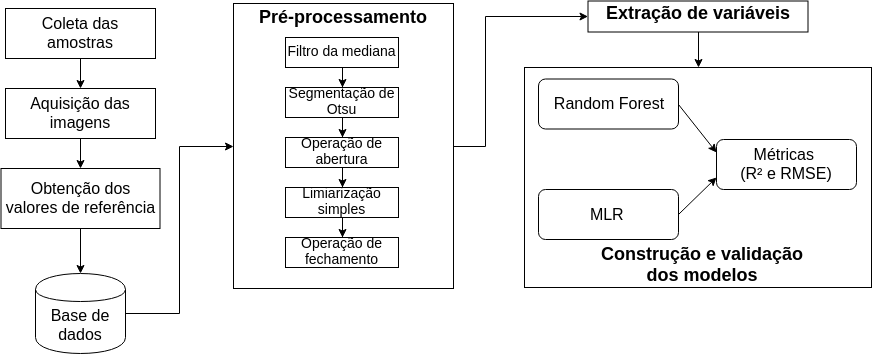
\includegraphics[scale=0.5]{img/diag.png}
    \legend{\textbf{Fonte:} (Autor, 2019).}
\end{figure}

\section{Descrição das amostras}

As mangas utilizadas no estudo foram das variedades ‘Palmer’ e ‘Tommy Atkins’, sendo duas das variedades mais produzidas no Vale do São Francisco (EMBRAPA SEMIÁRIDO, 2010). A variedade Palmer é caracterizada por frutos aromáticos e grandes, com peso de até 900 g, tom esverdeado ou arroxeado quando estão imaturos e cor vermelha quando maduros. Por outro lado, os frutos da variedade Tommy Atkins possuem um peso de aproximadamente 500 g e possuem uma coloração alaranjada, amarelada, avermelhada ou púrpura (NETO, 2009). 

As amostras foram coletadas de pomares comerciais da Fazenda SpecialFruit Importação e Exportação Ltda. em Petrolina e Juazeiro. Foram marcadas trinta plantas distribuídas em cinco fileiras de plantio de um lote do pomar. A cada quinze dias foram colhidos manualmente 60 frutos (dois de cada planta), para cada variedade, iniciando-se dos 35 dias após a floração\footnote{\label{ftnote:floracao} Etapa reprodutiva em que ocorre a diferenciação do meristema vegetativo para o floral, originando os componentes da flor (pétalas, estames e pistilo) (DUARTE FILHO et al., 1999).} até o ponto de colheita comercial adotado pela Fazenda, visando a construção de um modelo robusto de predição, onde mangas de diferentes estádios de maturação fossem utilizadas. \textcolor{red}{Ademais, as mangas foram armazenadas para a aquisição das imagens também na pós-colheita, com 10 e 20 dias após ela. (Como se deu essa parceria?)}

\section{Aquisição das imagens}

As imagens das mangas foram obtidas para cada lado da fruta, que foram colocadas em uma caixa de madeira compensada com um orifício no topo (Figura \ref{img:caixa}), onde foi posicionada uma câmera de 18 MP. O interior da caixa é preto fosco e contém uma superfície não reflexiva para o apoio das mangas. Na parte superior foram dispostos 3 LEDs brancos para a iluminação das amostras. O equipamento foi utilizado devido a uma parceria com o Laboratório de Energia na Agricultura (LENA) da UNIVASF.

\begin{figure}[H]
\centering
	\caption{Câmara para aquisição das imagens.}
	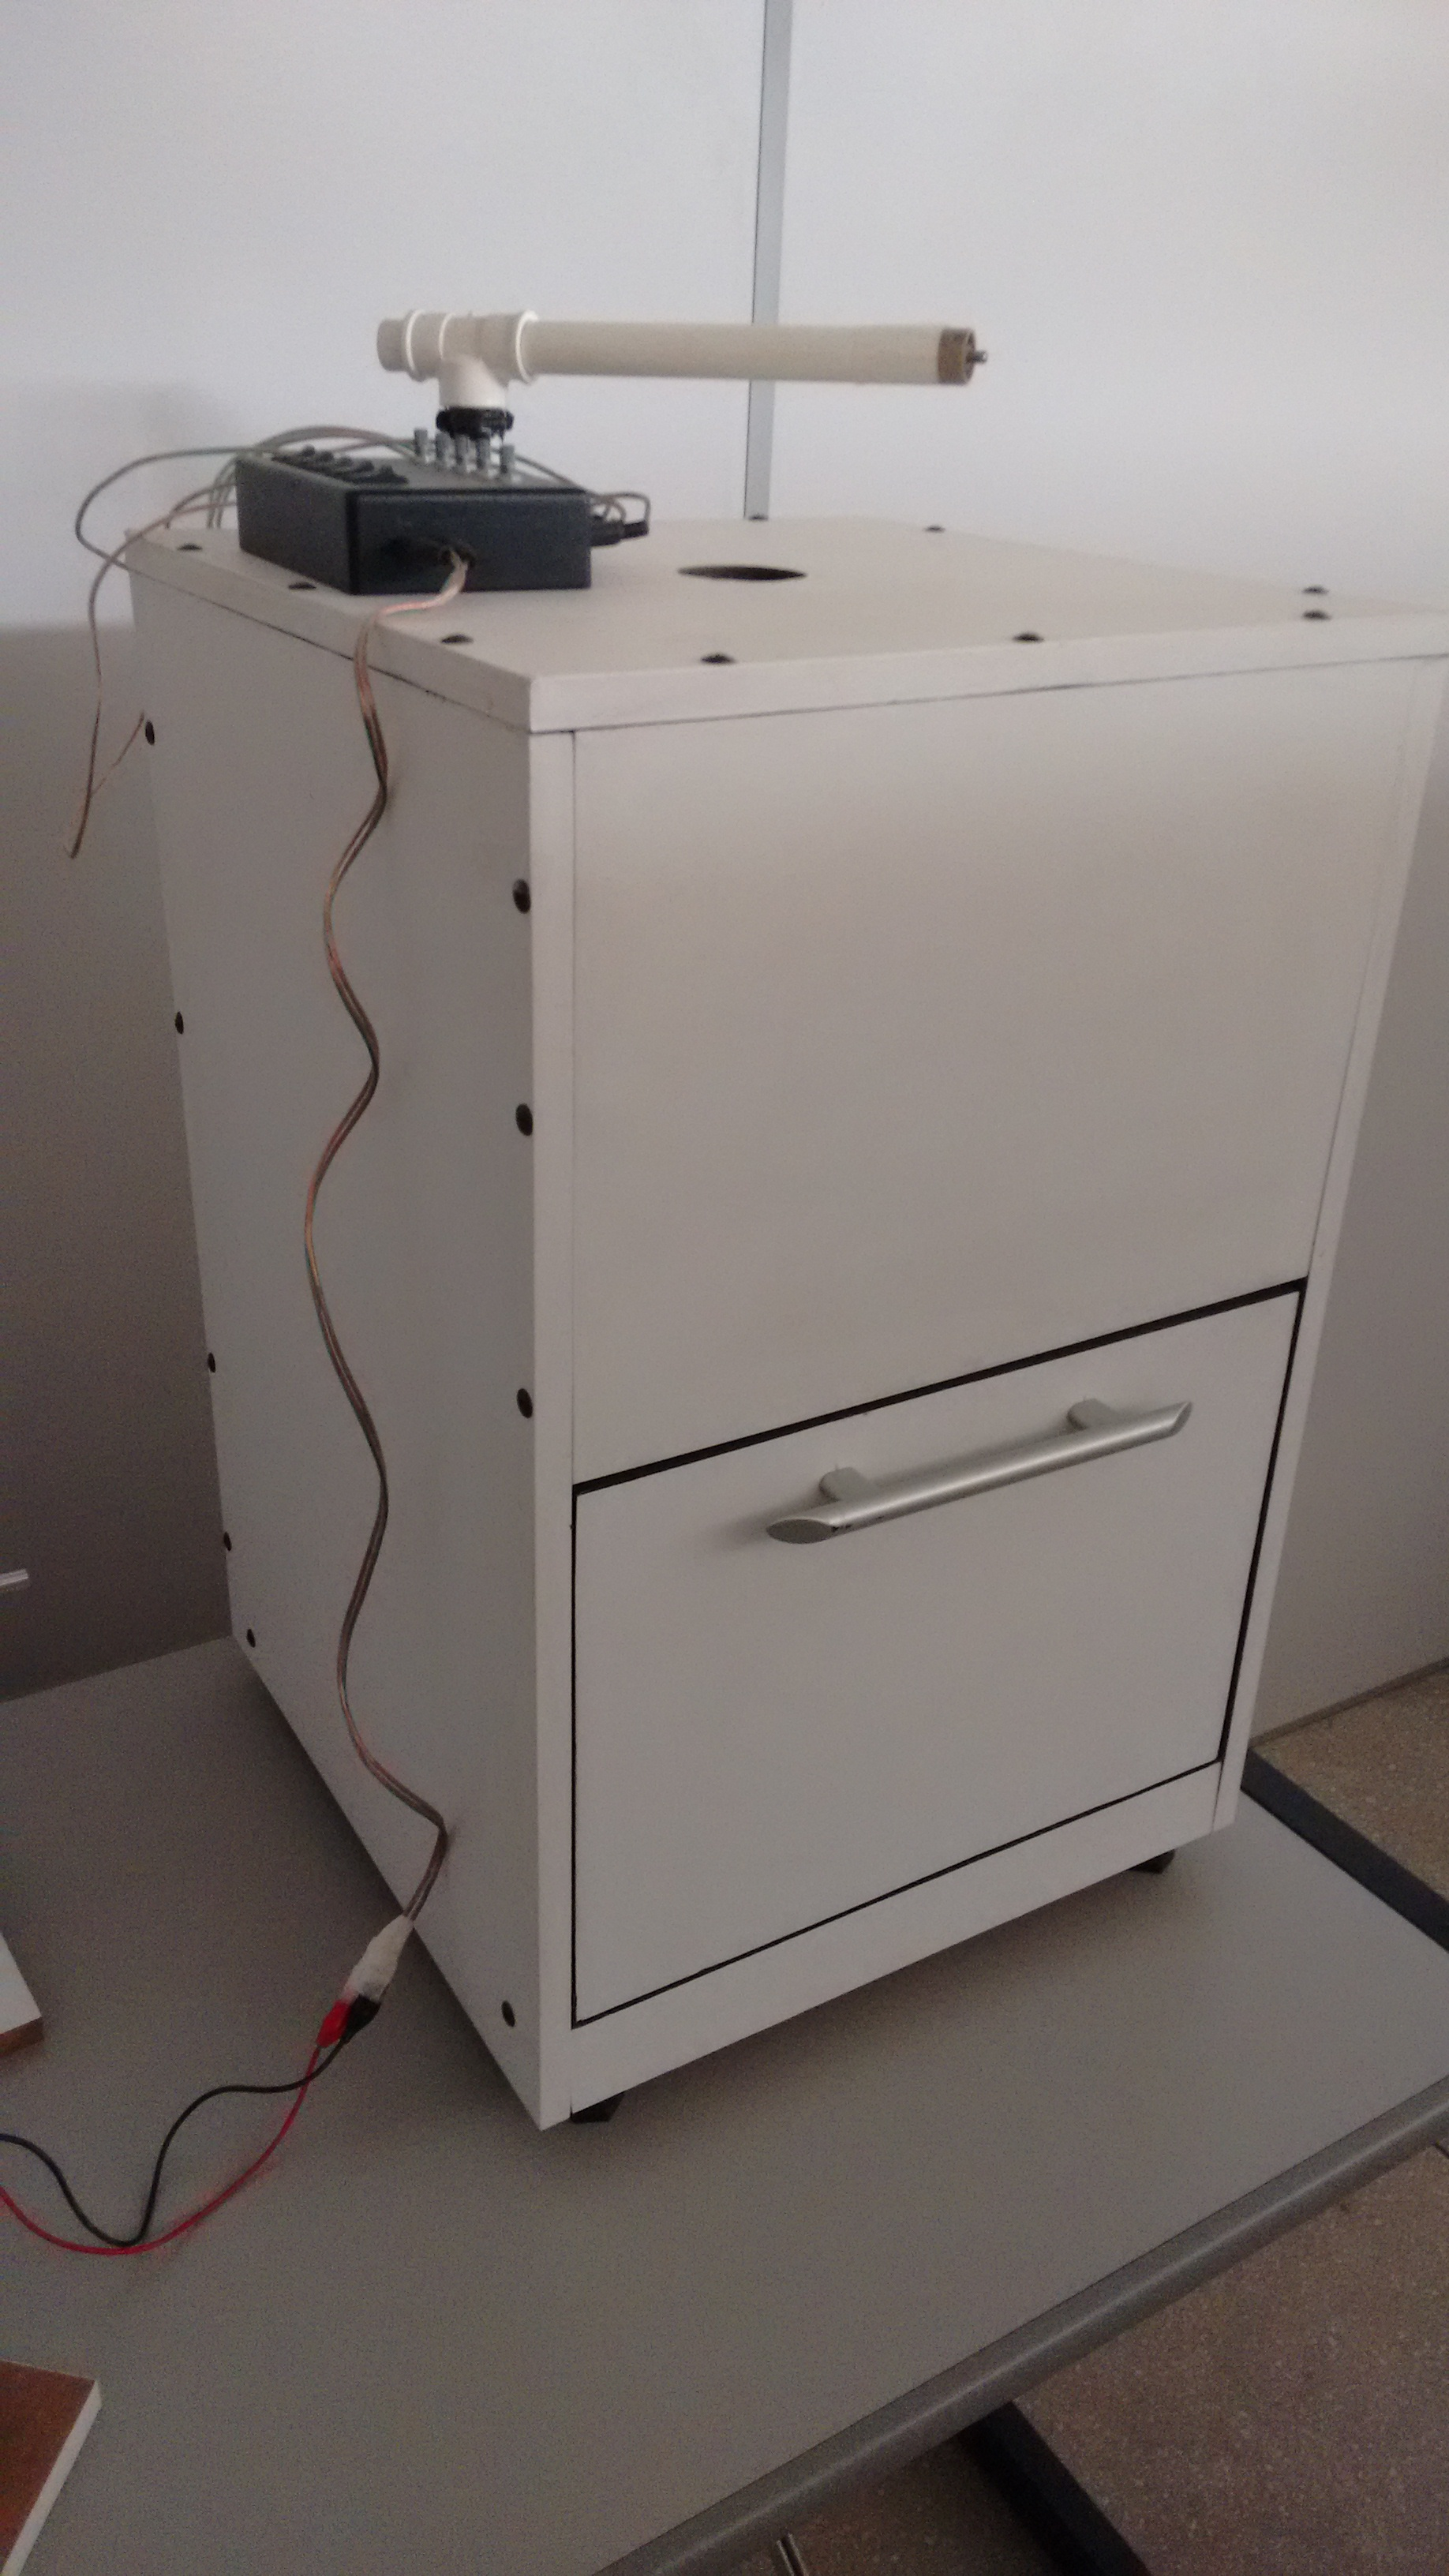
\includegraphics[scale=0.1]{img/caixa.jpg}
	\legend{\textbf{Fonte:} (Autor, 2019).}
\end{figure}

Foram tiradas fotos de 1230 mangas, sendo destas 480 da variedade ‘Tommy Atkins’ e 750 da ‘Palmer’. Como os dois lados de cada amostra foram fotografados, no total obtiveram-se 2460 imagens.

A aquisição foi realizada nos mesmos dias de coleta das frutas. Para a variedade ‘Tommy Atkins’, foram fotografadas 420 frutas até a data da colheita e 60 após ela. Para a 'Palmer', foram fotografadas 600 mangas até o dia da colheita e 150 após ela. A Figura \ref{img:palmer_tommy} exibe uma foto tirada para cada variedade.

\begin{figure}[!htb]
\centering
    \caption{\label{img:palmer_tommy} Fotos obtidas para cada variedade (a) Palmer (b) Tommy Atkins.}
    \subcaptionbox{(a)}{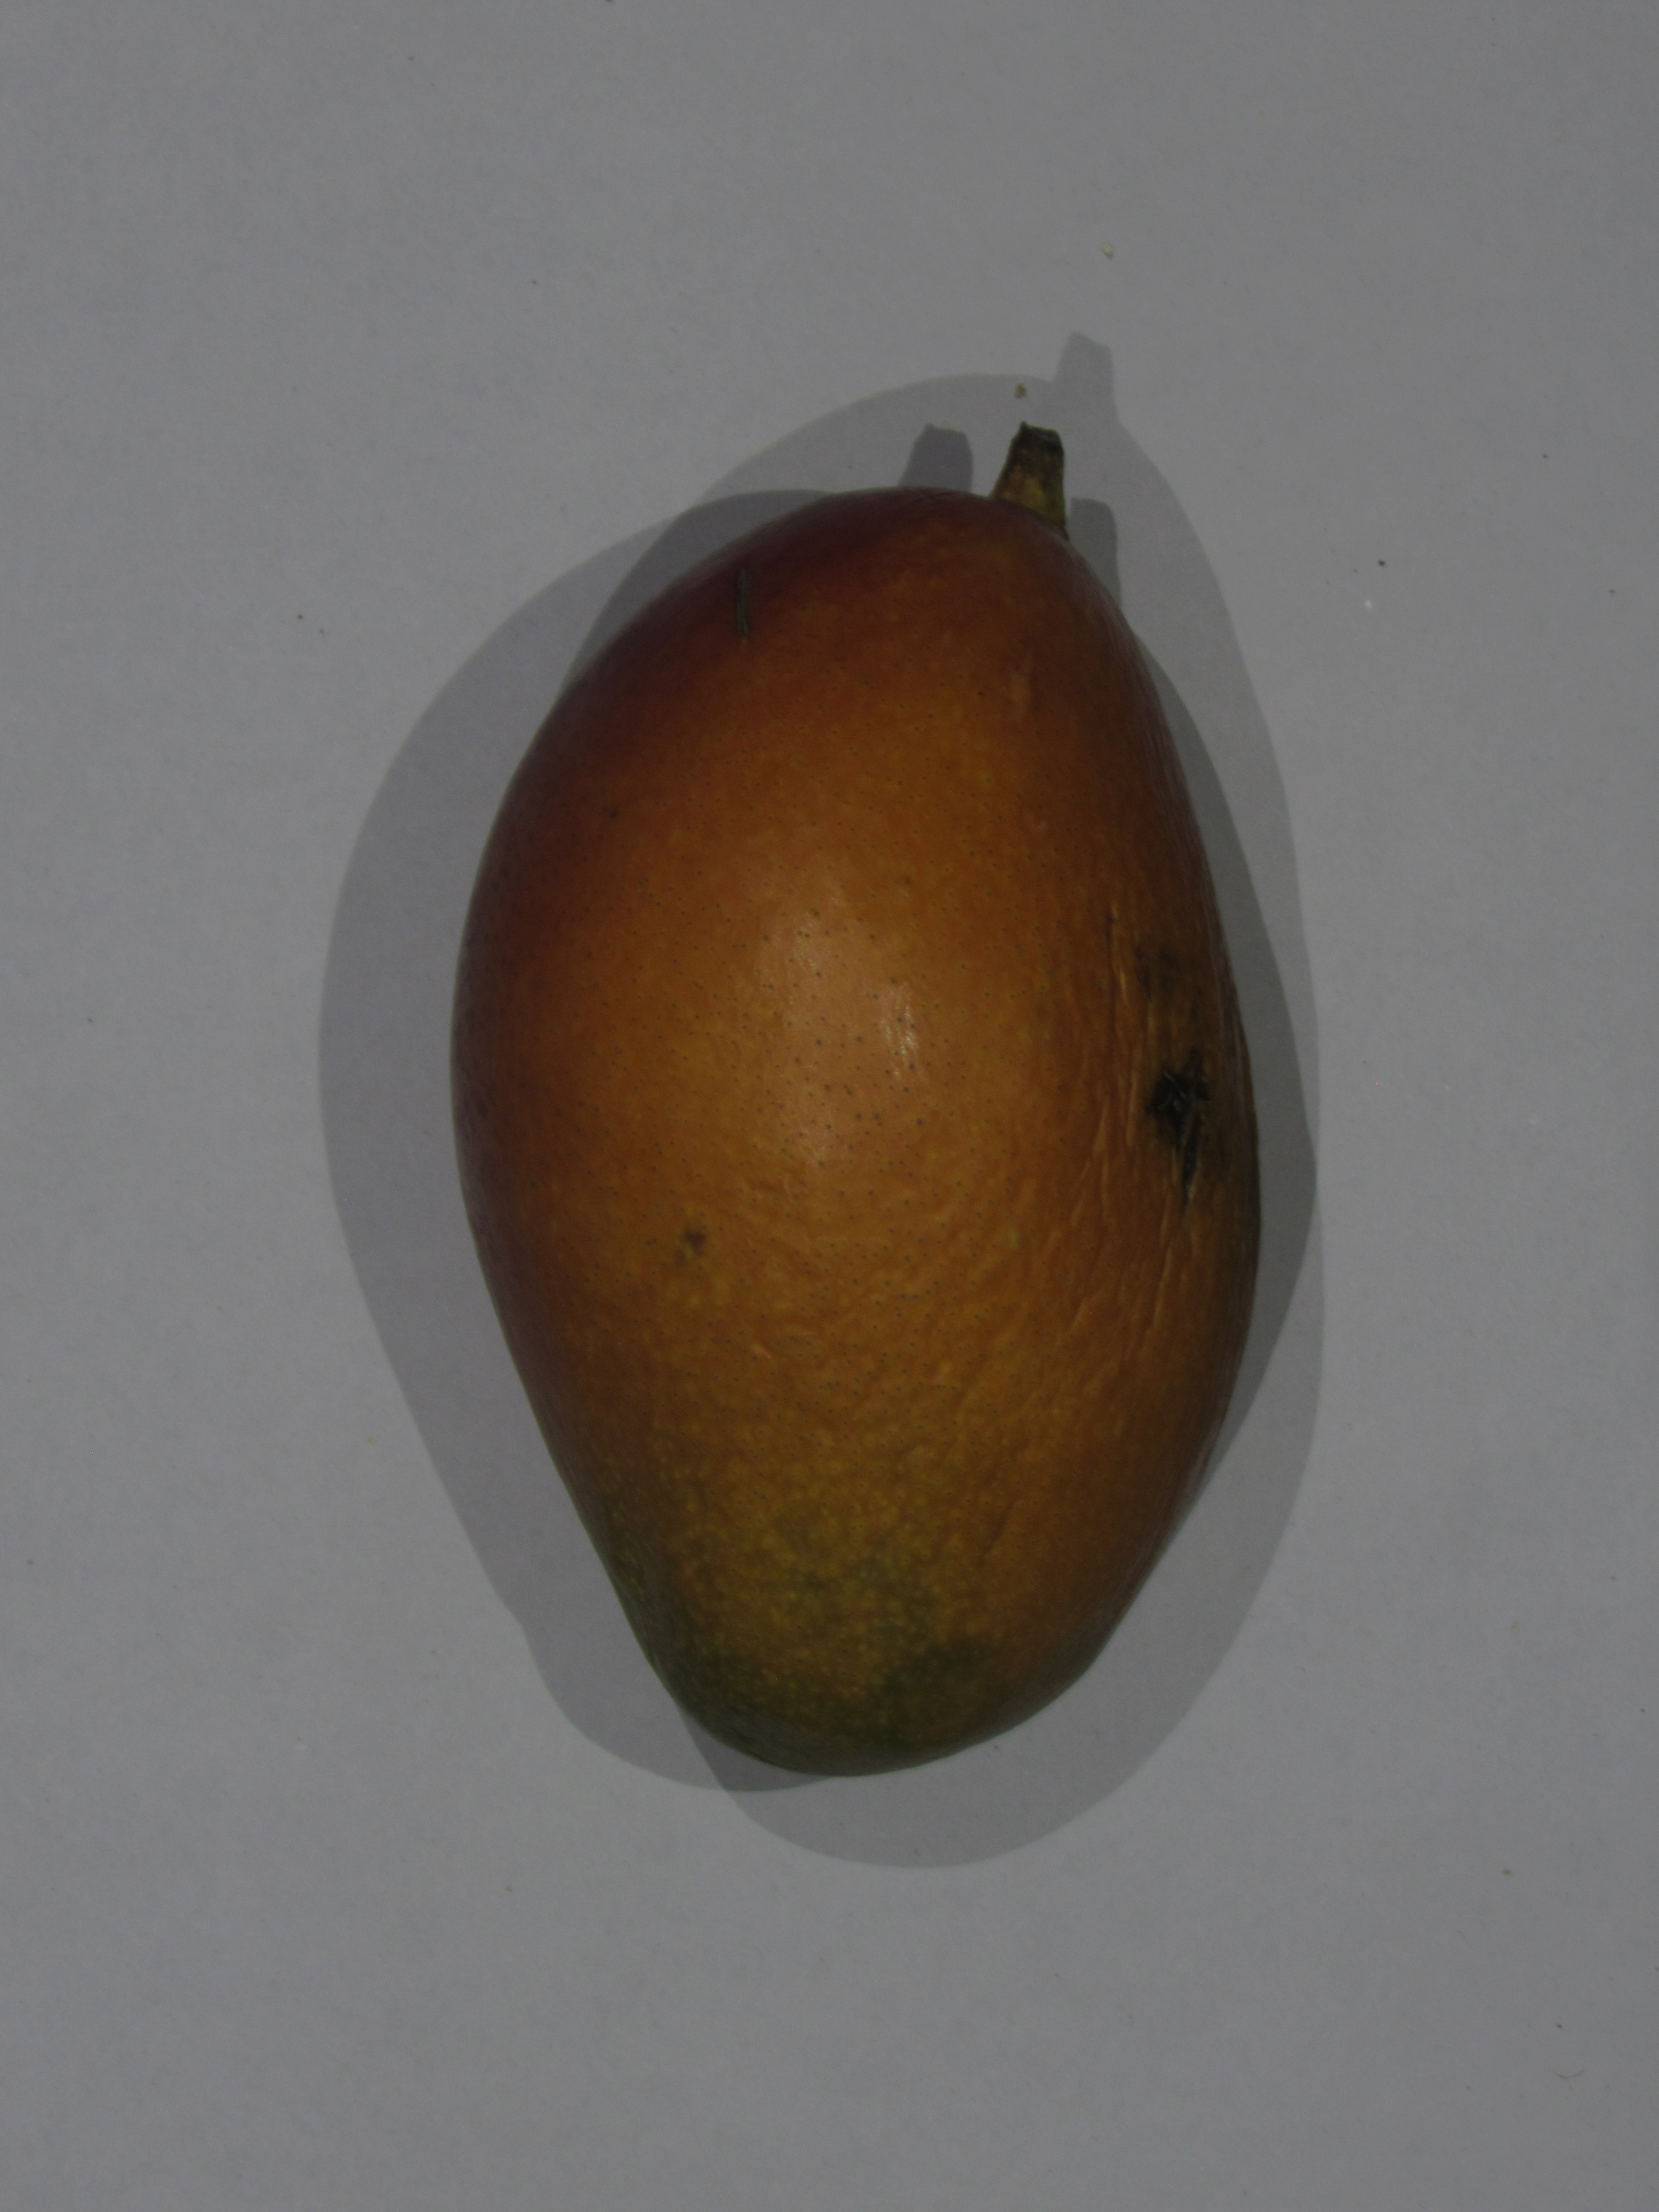
\includegraphics[scale=0.109]{img/palmer}}
    \subcaptionbox{(b)}{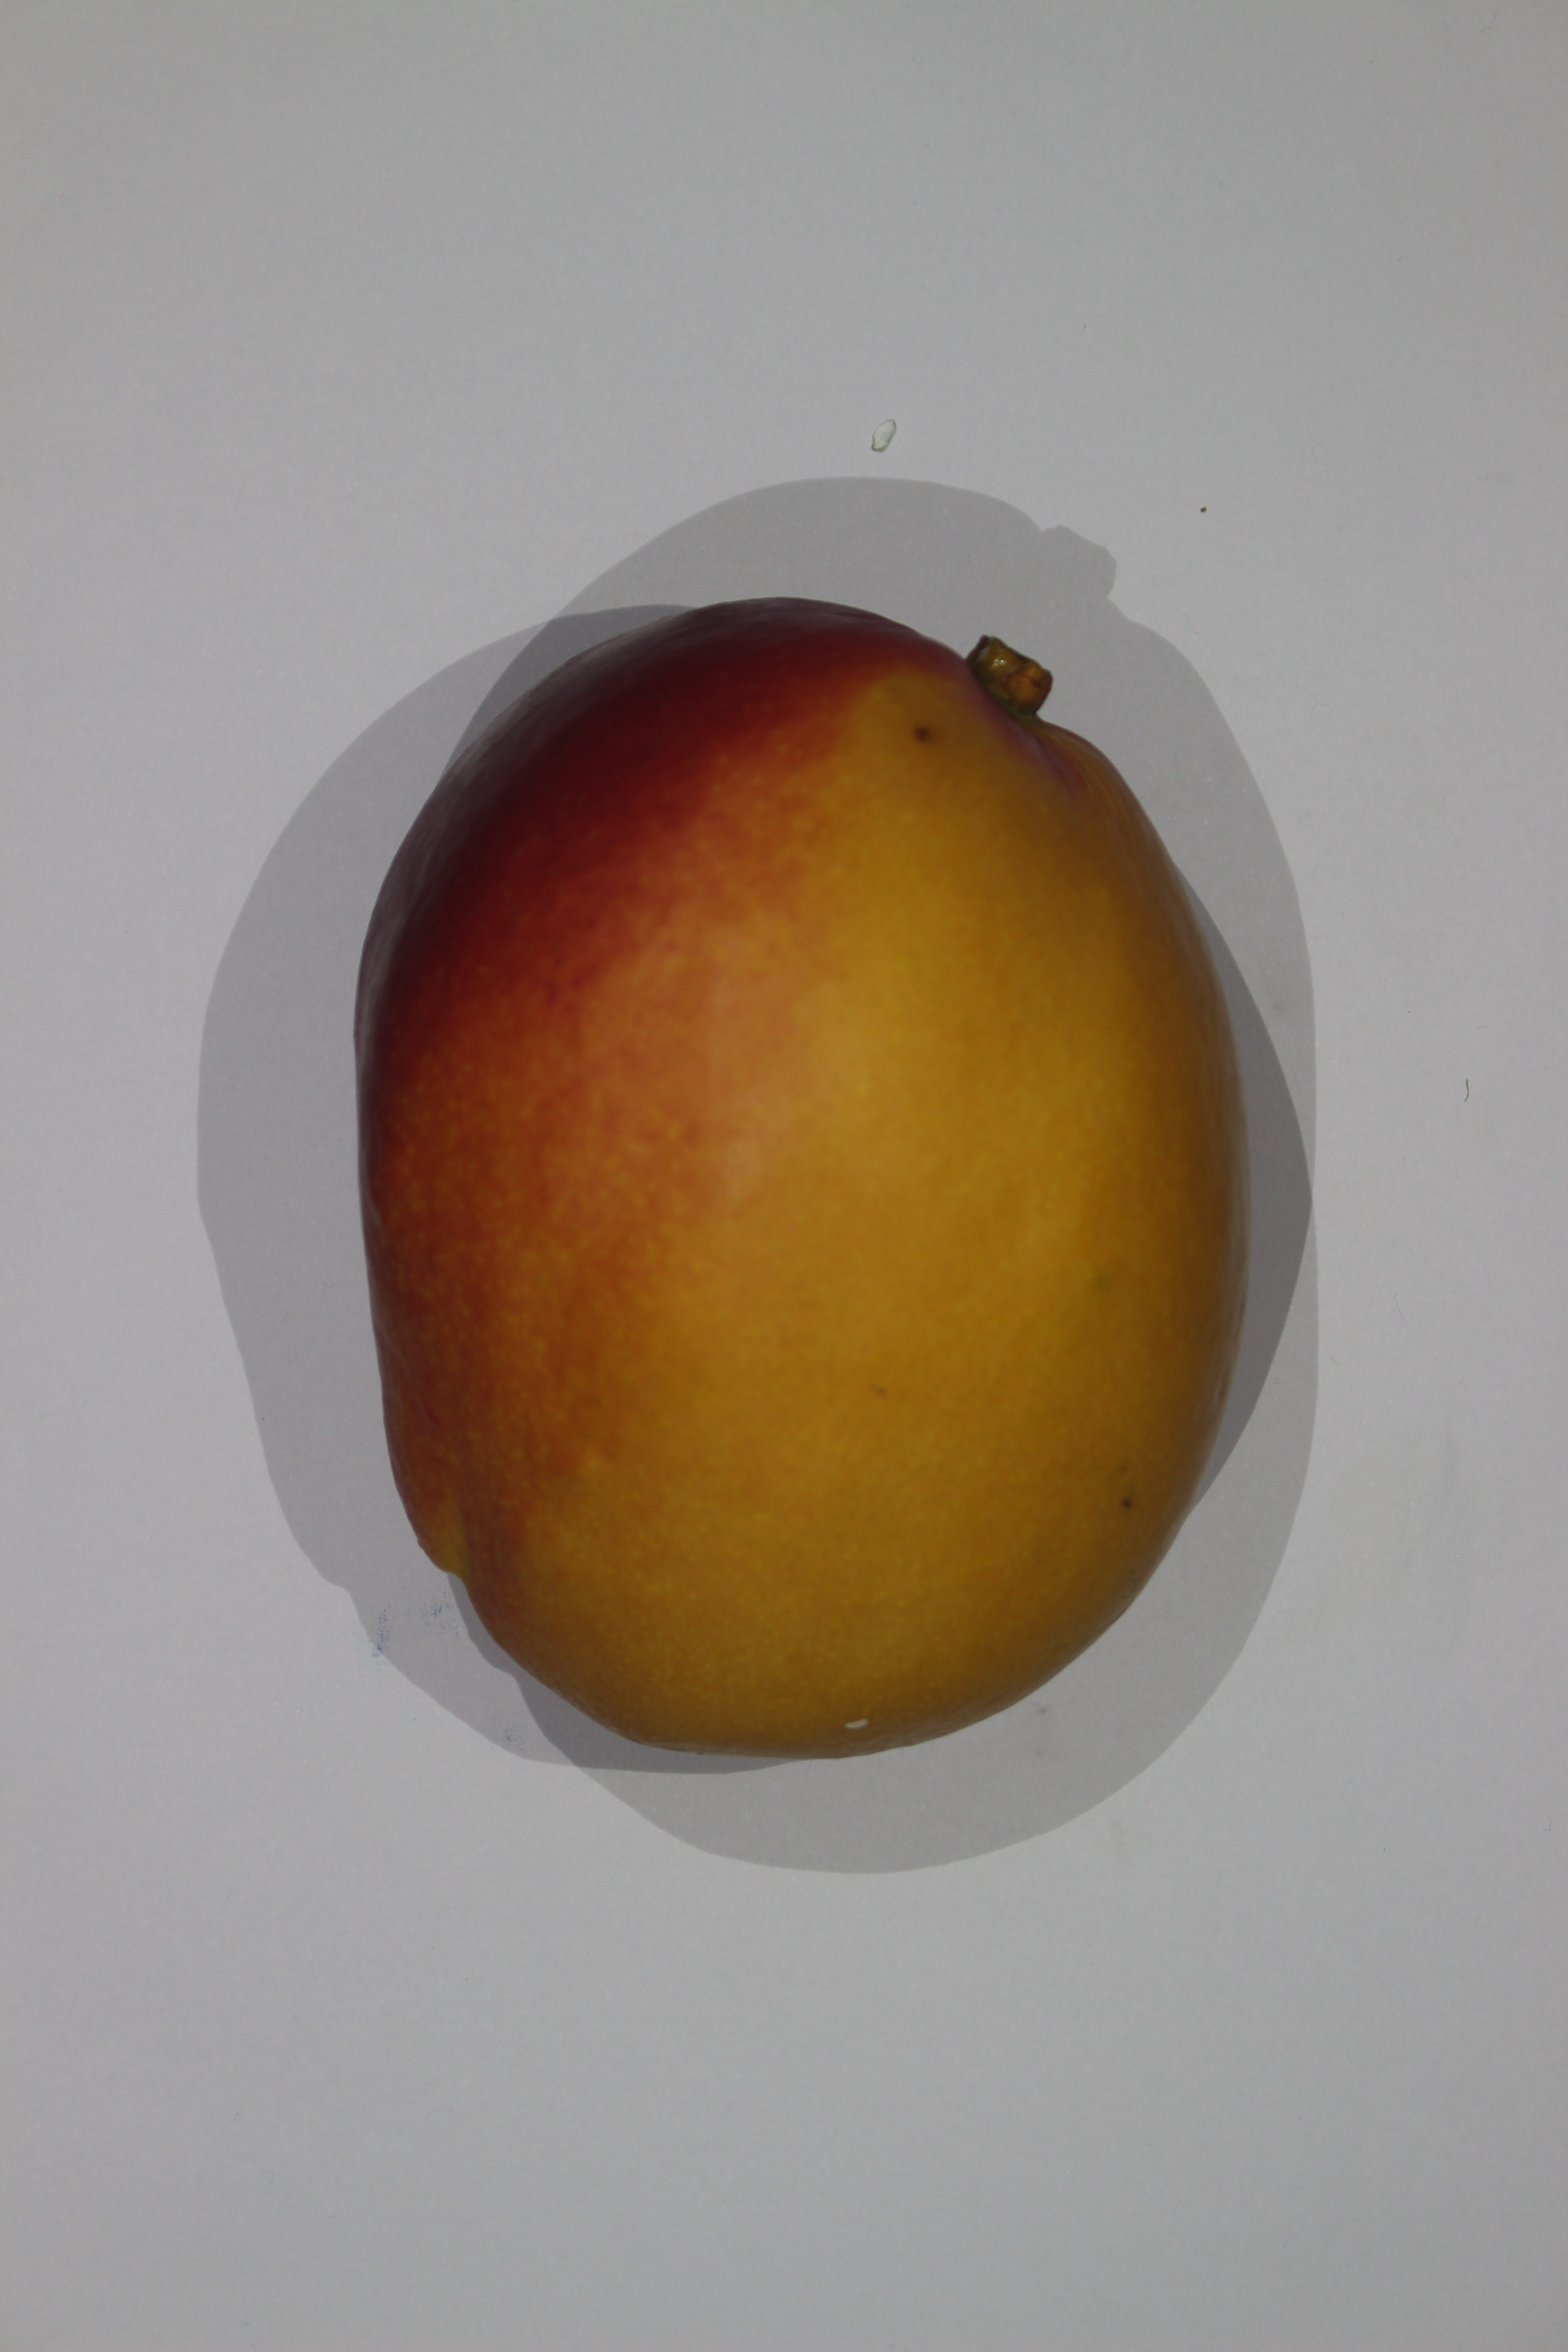
\includegraphics[scale=0.039]{img/tommy}}
    \legend{\textbf{Fonte: } (Autor, 2019).}
\end{figure}

\section{Obtenção dos valores de referência}

Os valores reais de SST foram obtidos segundo o procedimento do Instituto Adolfo Lutz (2008), sendo também adotado por Yahaya et al. (2015). Nele, as mangas têm inicialmente sua polpa homogeneizada e filtrada por uma centrífuga. O suco extraído é colocado em um refratômetro digital (HI 96804, Hanna Instruments, USA) para a quantificação de SST em ºBrix.

\section{Pré-processamento das imagens}

Como as imagens obtidas possuíam ruído e informações irrelevantes, foi necessário realizar o pré-processamento das mesmas. Foram testadas diferentes configurações de algoritmos, de forma a remover a maior quantidade possível de ruído sem perda de informações relevantes da imagem. Apesar de as fotos terem sido tiradas em um ambiente controlado, as imagens resultantes variaram quanto ao ruído nelas contido, devido ao acúmulo de sujeira na câmara com o passar das semanas do experimento. Sendo assim, as configurações das técnicas variaram para cada imagem.

A primeira técnica aplicada foi o filtro da mediana, visando a remoção de manchas contidas nas imagens. O tamanho de janela que garantiu uma melhor remoção de ruído na maioria das imagens foi de 11x11 pixels. Após isso, as imagens foram segmentadas através do algoritmo de Otsu, de forma que as mangas fossem isoladas do fundo. Com isso, notou-se nas imagens a presença de pequenos pontos que não foram removidos pelo filtro da mediana. Apesar de a remoção dos mesmos ter sido possível com uma segunda filtragem pela mediana, notou-se uma perda de detalhes na manga. Sendo assim, optou-se por empregar a operação de abertura, operação morfólogica através da qual pequenos pontos de uma imagem podem ser removidos. 

A utilização destas técnicas não garantiu uma remoção completa das sombras contidas na imagem. Assim, utilizou-se a limiarização simples para este fim, visto que a intensidade dos pixels correspondentes às sombras era, em geral, visivelmente menor que a intensidade dos pixels das mangas. Como a limiarização simples resultou na remoção de partes da manga, além das sombras delas, empregou-se a operação morfológica de fechamento para o preenchimento das mangas.

Por fim, foram traçados os contornos das mangas, visando a remoção de partes da imagem que não continham a fruta. A Figura \ref{fig:prep} mostra uma imagem original e pré-processada.

\begin{figure}[!htb]
\centering
    \caption{\label{fig:prep} Antes e depois do pré-processamento (a) Imagem original (b) Imagem resultante após utilização de técnicas de pré-processamento.}
    \subcaptionbox{(a)}{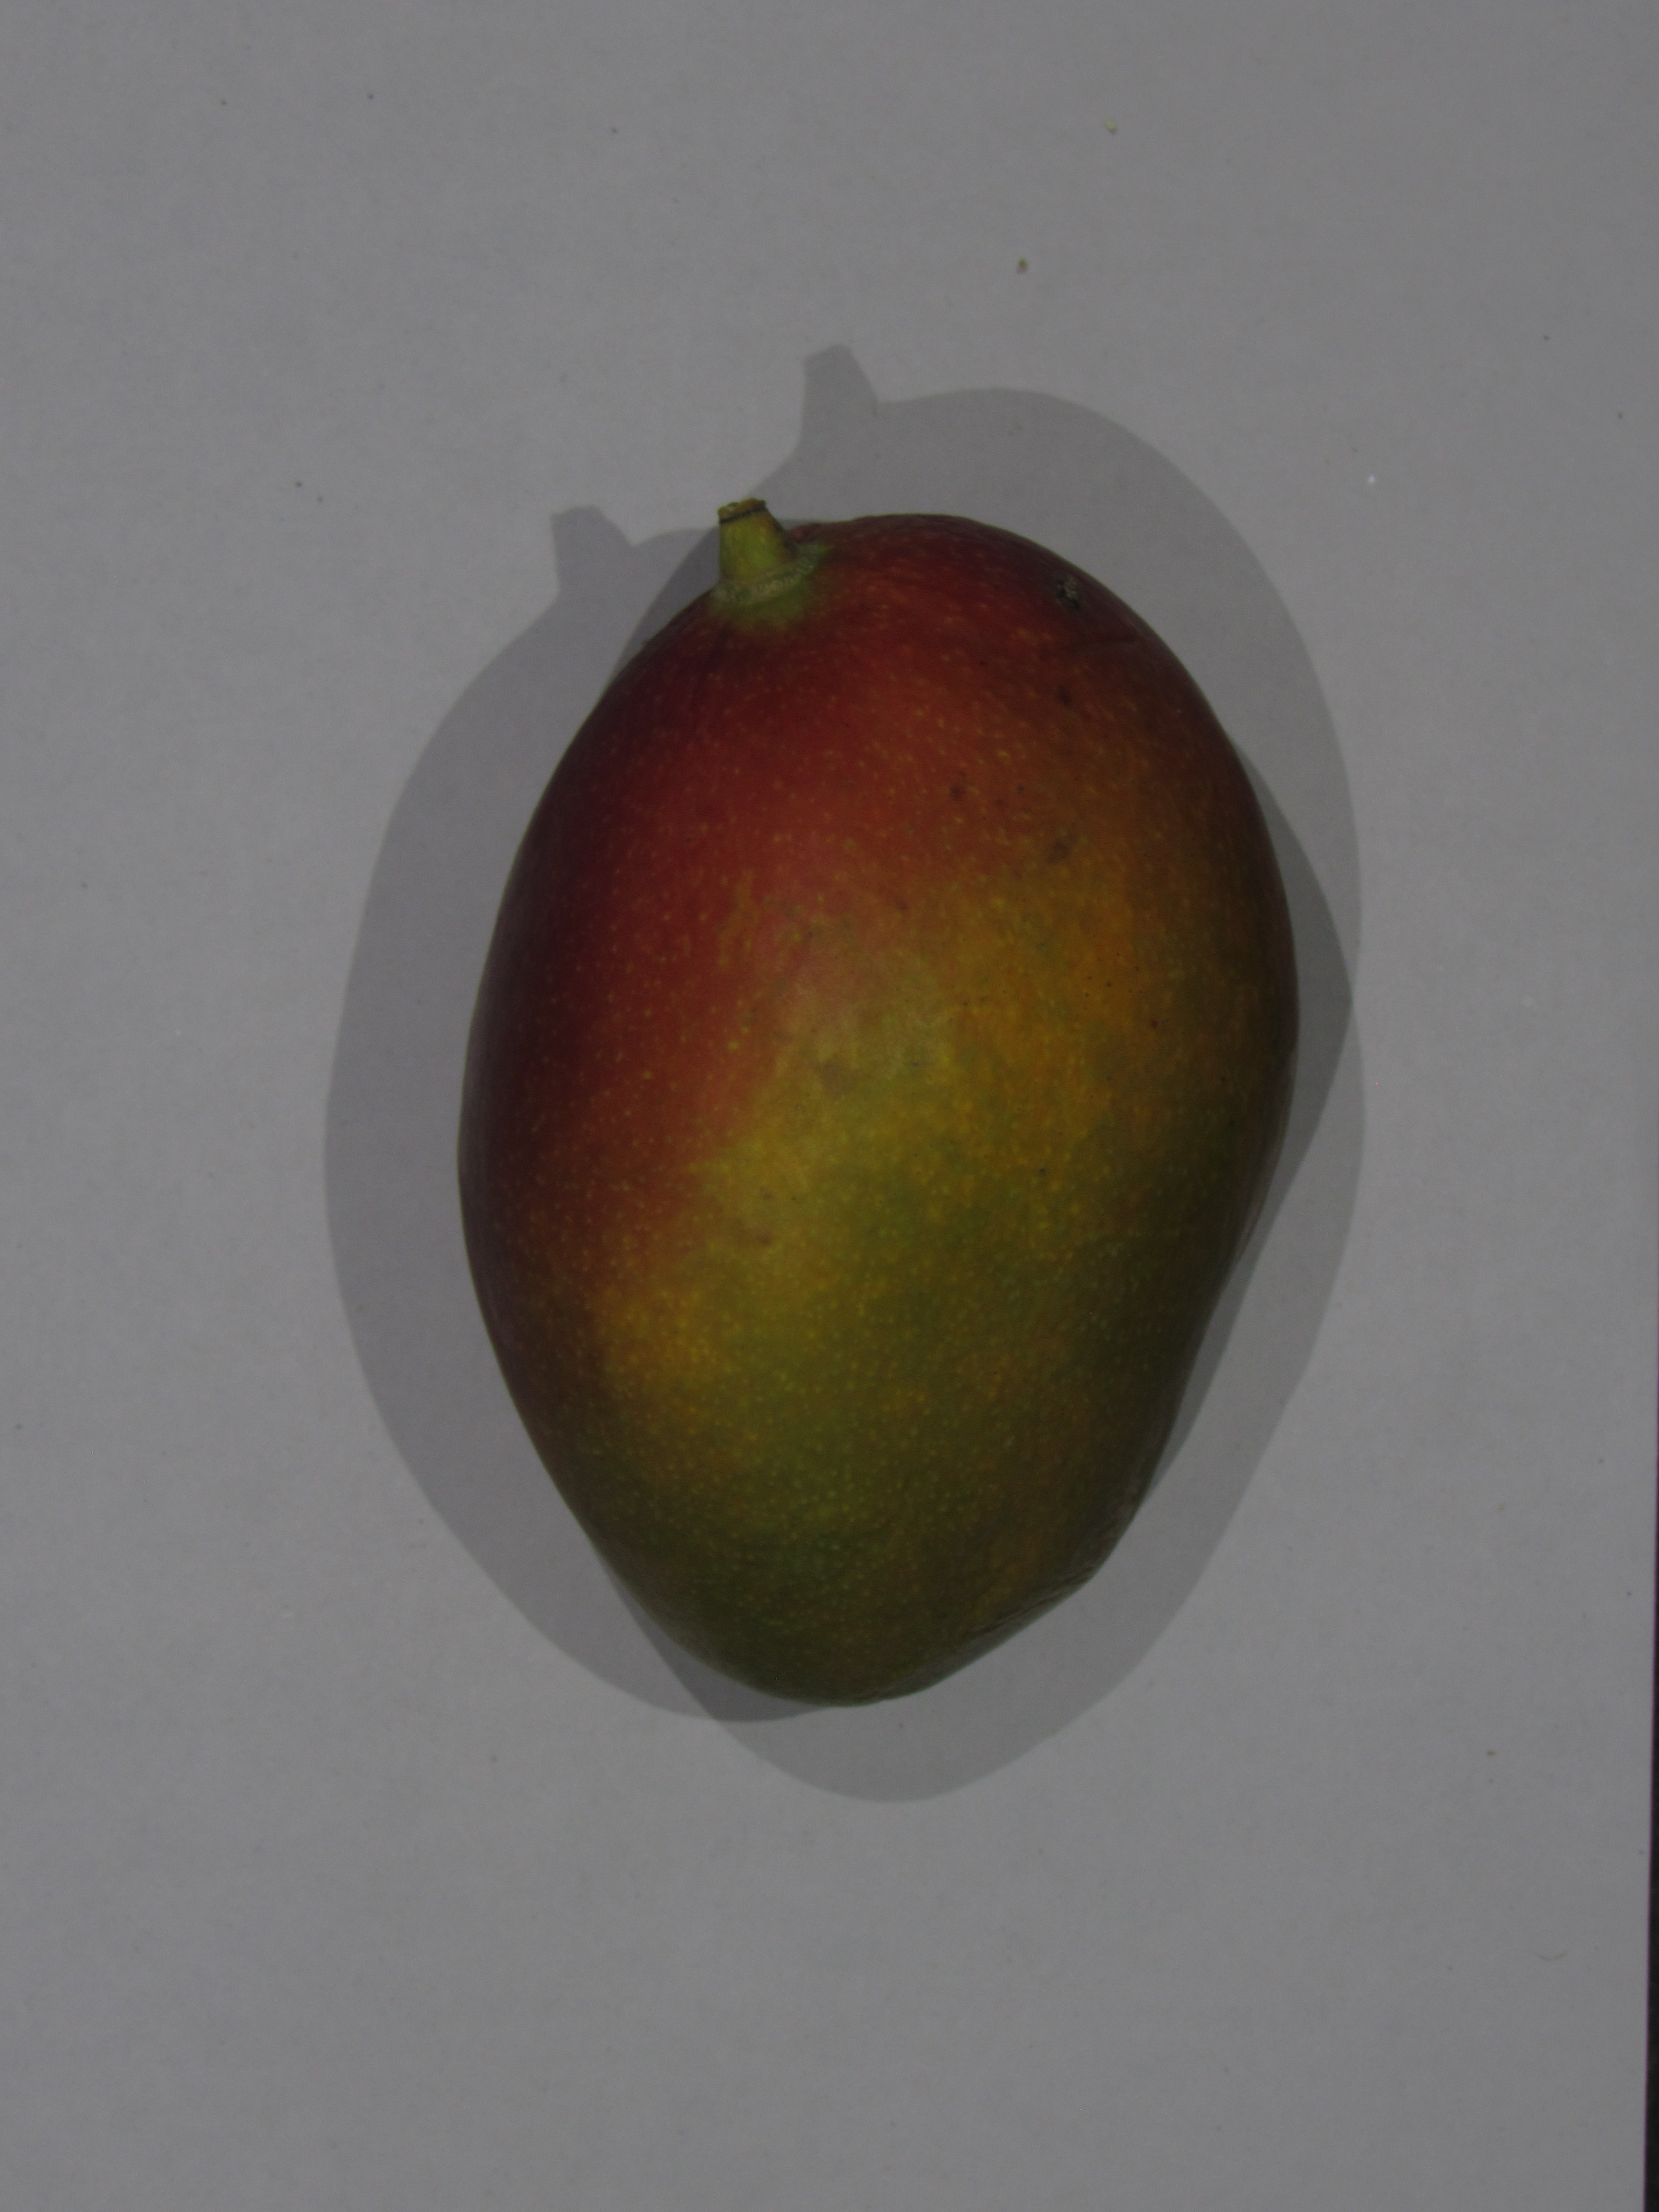
\includegraphics[scale=0.035]{img/sem_processamento.JPG}}
    \subcaptionbox{(b)}{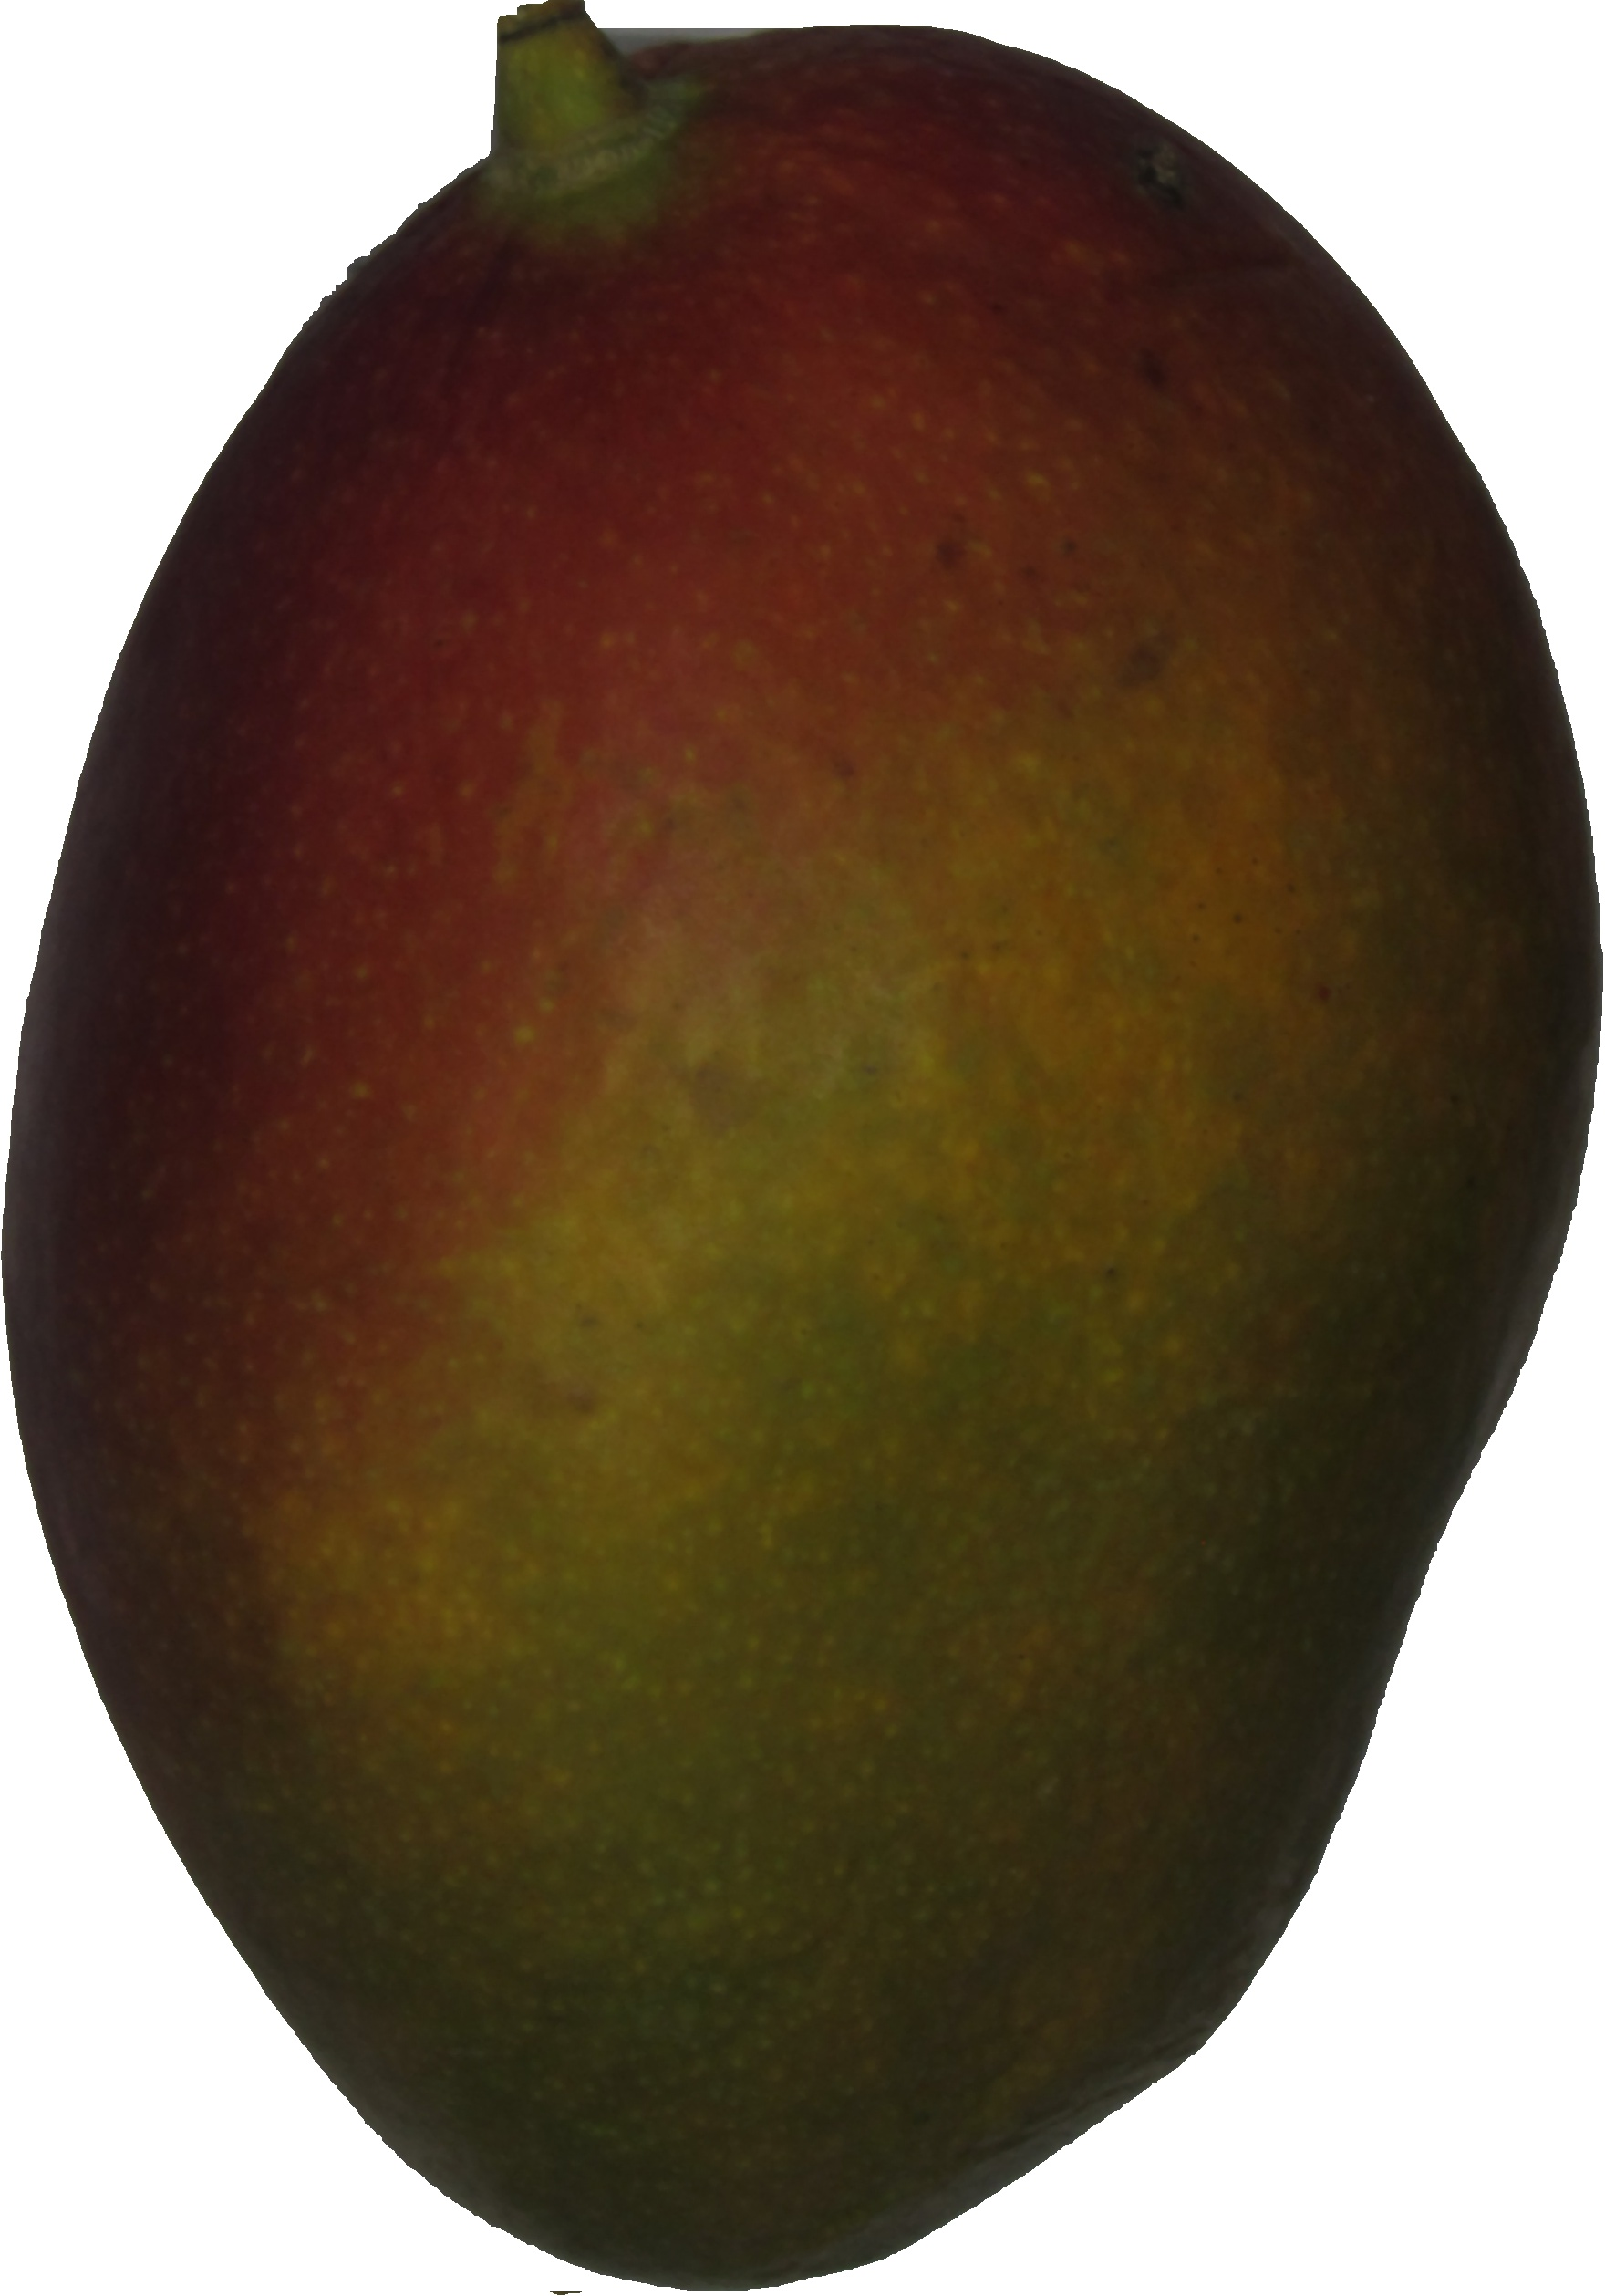
\includegraphics[scale=0.062]{img/processada.JPG}}
    \legend{\textbf{Fonte: } (Autor, 2019).}
\end{figure}

Posteriormente, as variáveis mencionadas na Tabela \ref{tab:artigos_att} foram extraídas para cada imagem. Todos os algoritmos de pré-processamento de imagens, assim como a extração de variáveis, foram realizados através da linguagem de programação Python, com o auxílio da biblioteca OpenCV.

\section{Construção dos modelos}

Antes da construção dos modelos foi realizada uma reamostragem das imagens, devido ao desbalanceamento presente na base de dados. Como havia 600 imagens de mangas tiradas antes da colheita e apenas 240 imagens tiradas após ela, foi feita uma repetição das imagens deste período até que fosse obtida uma quantidade igual de imagens nos dois períodos.

Assim, foram treinadas Random Forests para cada subconjunto de variáveis definido na Tabela \ref{tab:artigos_att}, além do subconjunto que reúne todas as variáveis, para a determinação do SST. Além disso, também foram construídos modelos com Regressão linear, para comparação direta com os melhores modelos da literatura.

% \subsection{Subseção de exemplo 1 - Referenciando seções} \label{subsec:subsec1}


%--------------------------------------------------------------------------------------
% Insere a seção de cronograma
% Está comentada porque só é necessária no TCC I
%--------------------------------------------------------------------------------------

%\section{Cronograma} \label{sec:crono}

%A tabela \ref{tab:cronograma} mostra o cronograma de atividades a serem executadas para o TCC II, com base no calendário de 201X.Y da UNIVASF.

%\newpage
%\begin{table}[!thb]
%	%\huge
%    \centering
%    \caption{\label{tab:cronograma} Cronograma das atividades previstas para o TCC II}
%%    \begin{adjustbox}{max width=\textwidth}
%    \begin{tabular}{p{6.5cm}|c|c|c|c|c|c}
%    \toprule
%    \textbf{Atividade}                      & Nov & Dez & Jan & Fev & Mar & Abr \\ \hline
%    Implementar o banco de dados              & X    & X     &       &        &          &          \\ \hline
%    Desenvolver a API HTTP RESTful                      &   X   & X     &       &        &          &          \\ \hline
%    Implementar o serviço de captura de dados        &      &      & X     &   X     &          &          \\ \hline
%    Desenvolver a aplicação \textit{Web/mobile} para exibição dos dados         &      &      & X     &   X     &     X     &          \\ \hline
 %   Teste do sistema            &      &       &       &        & X        &          %\\ \hline
 %   Escrita do TCC II                       &   X   & X     & X     & X      & X        & X        \\ \hline
%   Defesa do TCC II                        &      &       &       &        &          & X       \\
%    \bottomrule
 %   \end{tabular}
 %   \end{adjustbox}
%    \legend{\textbf{Fonte:} O autor.}
%\end{table}


		\chapter{Resultados} \label{ch:RD}

A estatística descritiva do atributo SST é mostrada na Tabela \ref{tbl:sst_stat}, onde nota-se uma grande variabilidade nos dados. Dessa forma, é possível construir um modelo robusto capaz de realizar a predição deste atributo para diferentes estádios de maturação da manga.

\begin{table}[H]
\centering
\begin{tabular}{llllllll}
\hline
Dados     & Amostras & M\'edia & M\'in & M\'ax & Amplitude & SD & Vari\^ancia   \\
\hline
SST     & 1200 & 9,83 &  3,8 &  19,7 &  15,9 &  4,5 &  20,24 \\
\hline
\end{tabular}
\caption{Estatística descritivas dos valores de referência de SST.} \label{tbl:sst_stat}
\end{table}

Inicialmente os modelos construídos na literatura foram replicados para as mangas 'Palmer', para a comparação dos resultados. No trabalho de Khairunniza-Bejo e Kamarudin (2011), o atributo SST foi previsto em mangas 'Chokanan' a partir do espaço de cores HSV. Os autores construíram modelos de Regressão Linear Simples para cada canal deste espaço de cor, e obtiveram como melhor resultado um coeficiente de correlação igual a -0,92 para o canal matiz. Assim, para as mangas da variedade 'Palmer', também foi construída uma Regressão linear com o atributo matiz como entrada. Entretanto, esperava-se um resultado inferior aos obtidos pelos autores, visto que, para as mangas 'Palmer', o atributo matiz não varia linearmente. A Figura \ref{fig:hue_sst} mostra a variação do SST de acordo com a matiz. 

\begin{figure}[H]
\centering
	\caption{Variação do SST conforme a matiz.}
	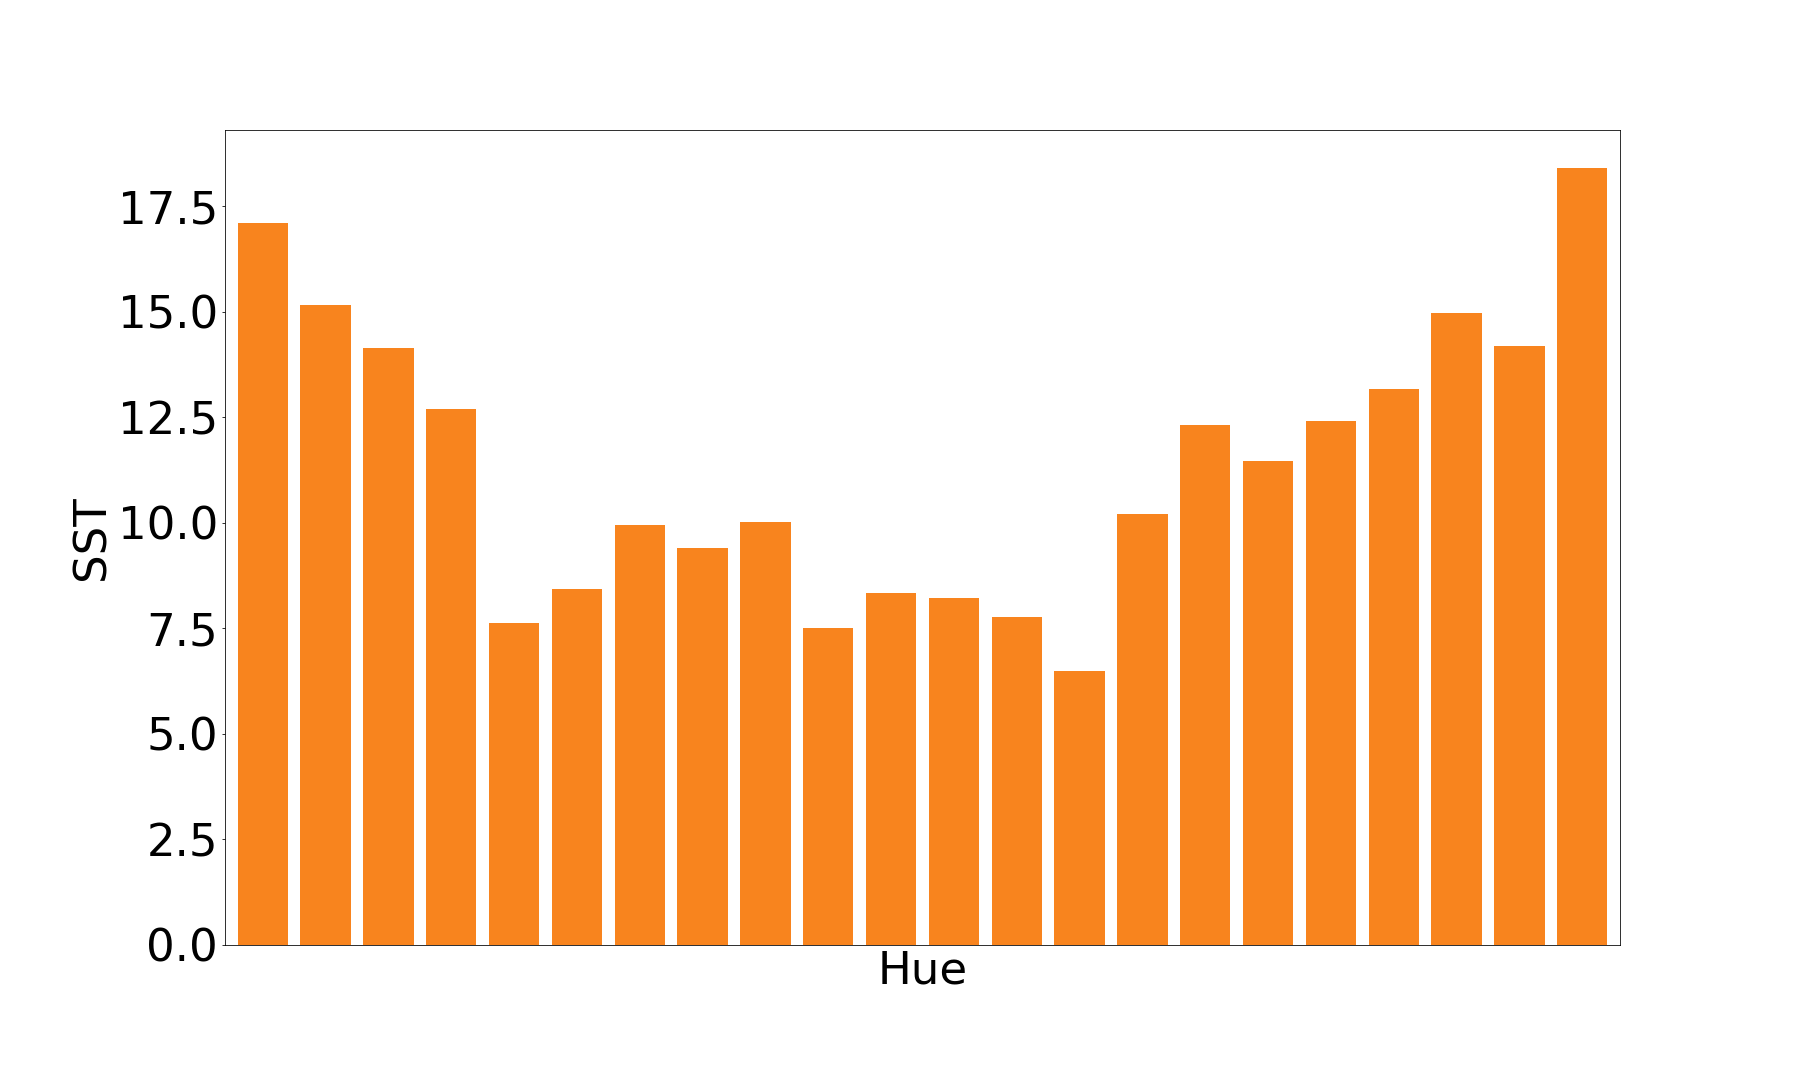
\includegraphics[scale=0.18]{img/hue_sst_palmer.png}
	\legend{\textbf{Fonte:} (Autor, 2019).}\label{fig:hue_sst}
\end{figure}

Conforme esperado, o coeficiente de correlação obtido para a Regressão linear foi muito inferior, com um valor igual a -0,1179. Na Figura \ref{fig:comp_hue} são mostradas a reta ajustada para as amostras do presente estudo e a reta ajustada pelos autores Khairunniza-Bejo e Kamarudin (2011).

\begin{figure}[H]
\centering
    \caption{\label{fig:comp_hue} Modelos de Regressão linear construídos para o atributo matiz (a) Presente estudo (b) Trabalho de Khairunniza-Bejo e Kamarudin (2011).}
    \subcaptionbox{}{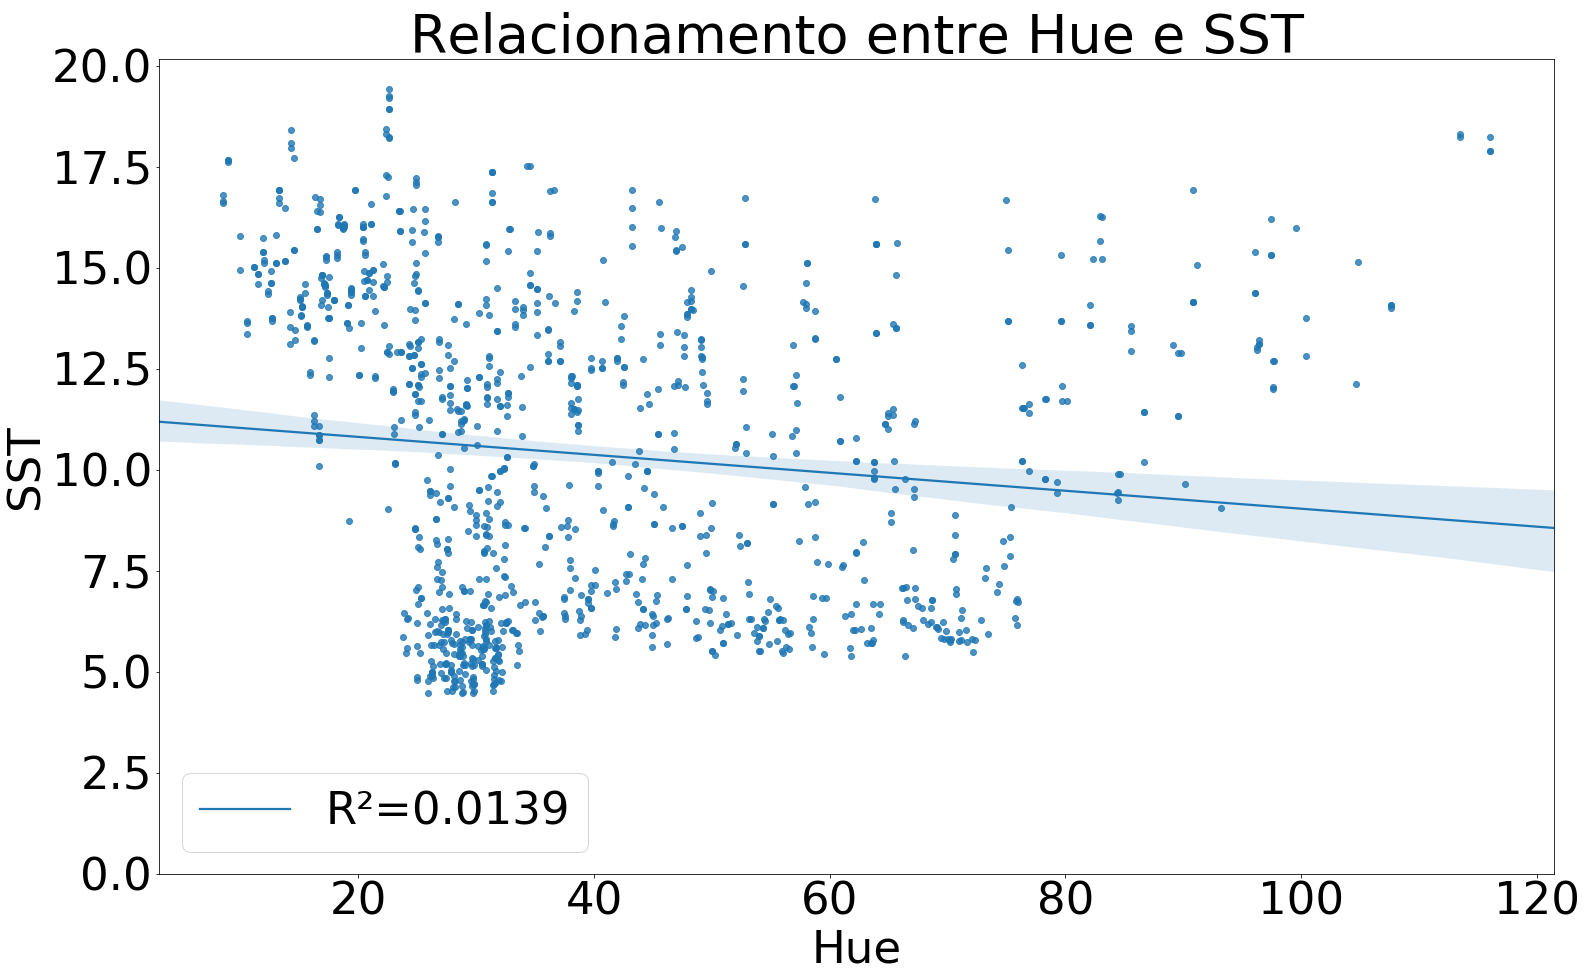
\includegraphics[scale=0.133]{img/scatter_sst_hue_palmer.png}}
    \subcaptionbox{}{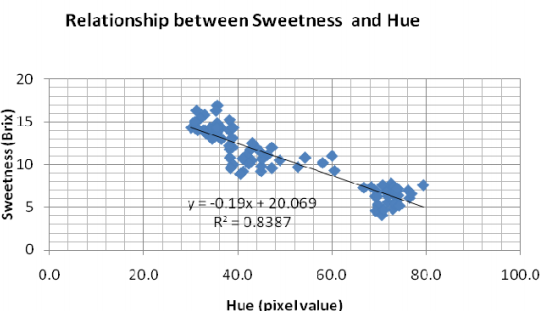
\includegraphics[scale=0.36]{img/sst_lit_hue.png}}
    \legend{\textbf{Fonte: } (Autor, 2019).}
\end{figure}

Devido ao relacionamento não linear entre a matiz e SST, esperava-se que com a \textit{Random Forest} fosse obtido um resultado superior. Os valores de $R$ e $RMSE$ obtidos por ela, assim como pela Regressão linear, são mostrados na Figura \ref{fig:fold_sst_hue}, para cada \textit{fold}.

\begin{figure}[H]
\centering
	\caption{Métricas obtidas para cada \textit{fold}, obtidos para as duas técnicas de inferência (a) Coeficiente de correlação (R) (b) RMSE.}
	\subcaptionbox{}{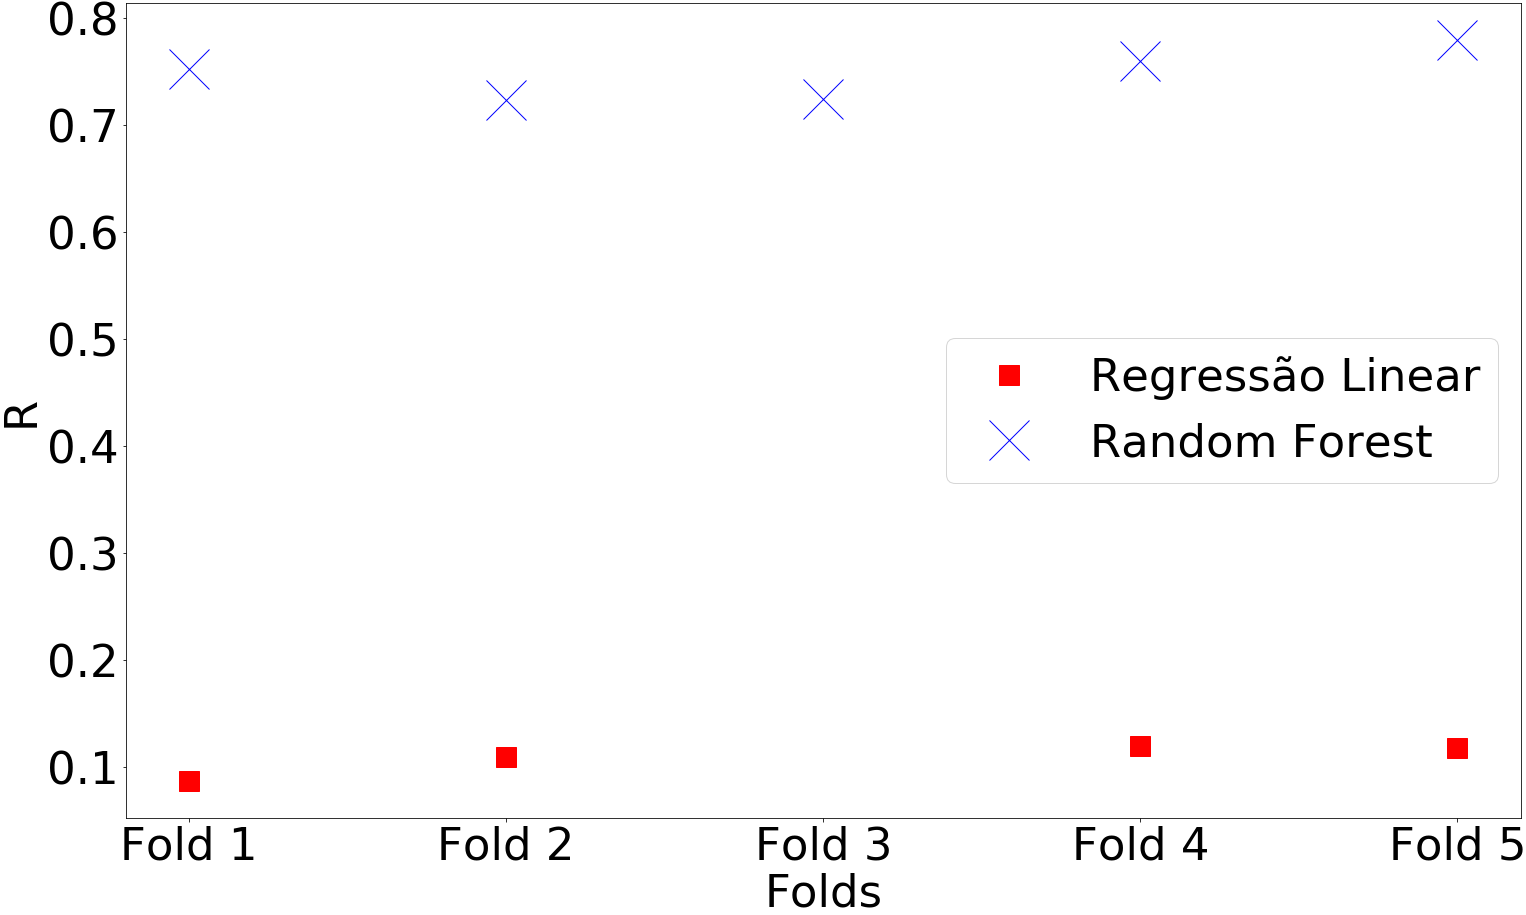
\includegraphics[scale=0.15]{img/fold_r_sst_hue_palmer.png}}
	\subcaptionbox{}{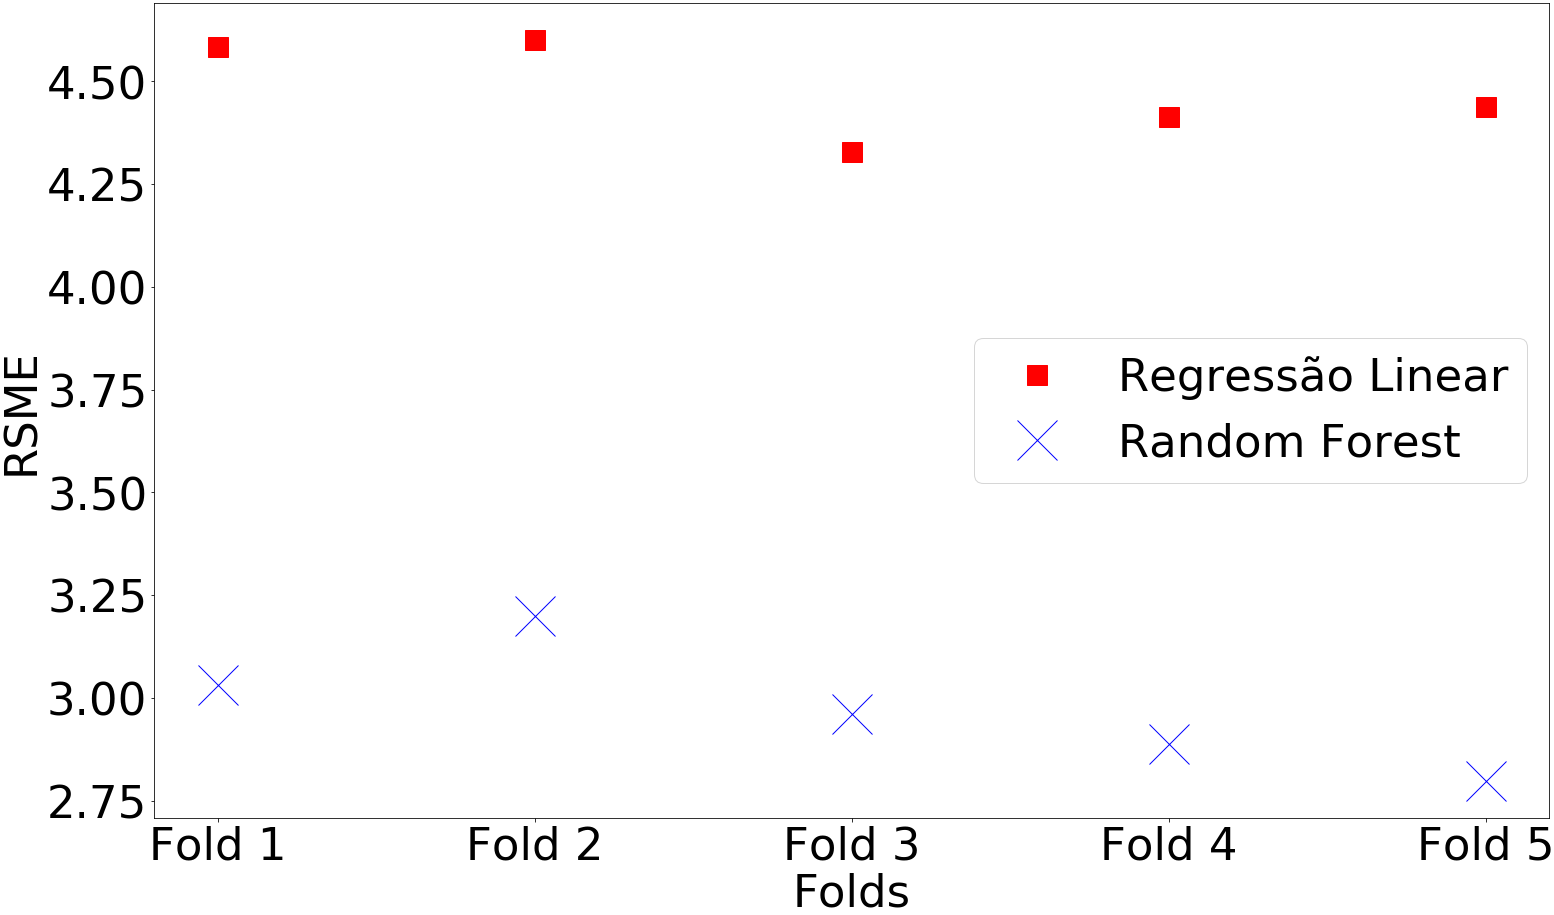
\includegraphics[scale=0.15]{img/fold_rmse_sst_hue_palmer.png}}
	\legend{\textbf{Fonte:} (Autor, 2019).}\label{fig:fold_sst_hue}
\end{figure}

Apesar de a \textit{Random Forest} ser claramente superior, como esperado, o resultado ainda não é razoável. O coeficiente de correlação ainda mostra-se bastante abaixo que o obtido pelos autores Khairunniza-Bejo e Kamarudin (2011), enquanto que o RMSE é muito maior que o obtido por eles (0,033 ºBrix). Para as mangas da variedade 'Palmer', vê-se que este atributo não é suficiente para a determinação de SST como foi para as mangas da variedade 'Chokanan'.

Por outro lado, os autores Yahaya et al. (2015) testaram o espaço de cores RGB e obtiveram um coeficiente de correlação igual a 0,814 e RMSE igual a 1,218 ªBrix. Para verificar se existe uma relação linear entre as variáveis RGB extraídas das mangas 'Palmer' e o SST, foram plotadas as variações das mesmas, mostradas na Figura \ref{fig:rgb_sst}.

\begin{figure}[H]
\centering
    \caption{\label{fig:rgb_sst} Variação das variáveis RGB para o SST (a) Canal R (b) Canal G (c) Canal B.}
    \subcaptionbox{}{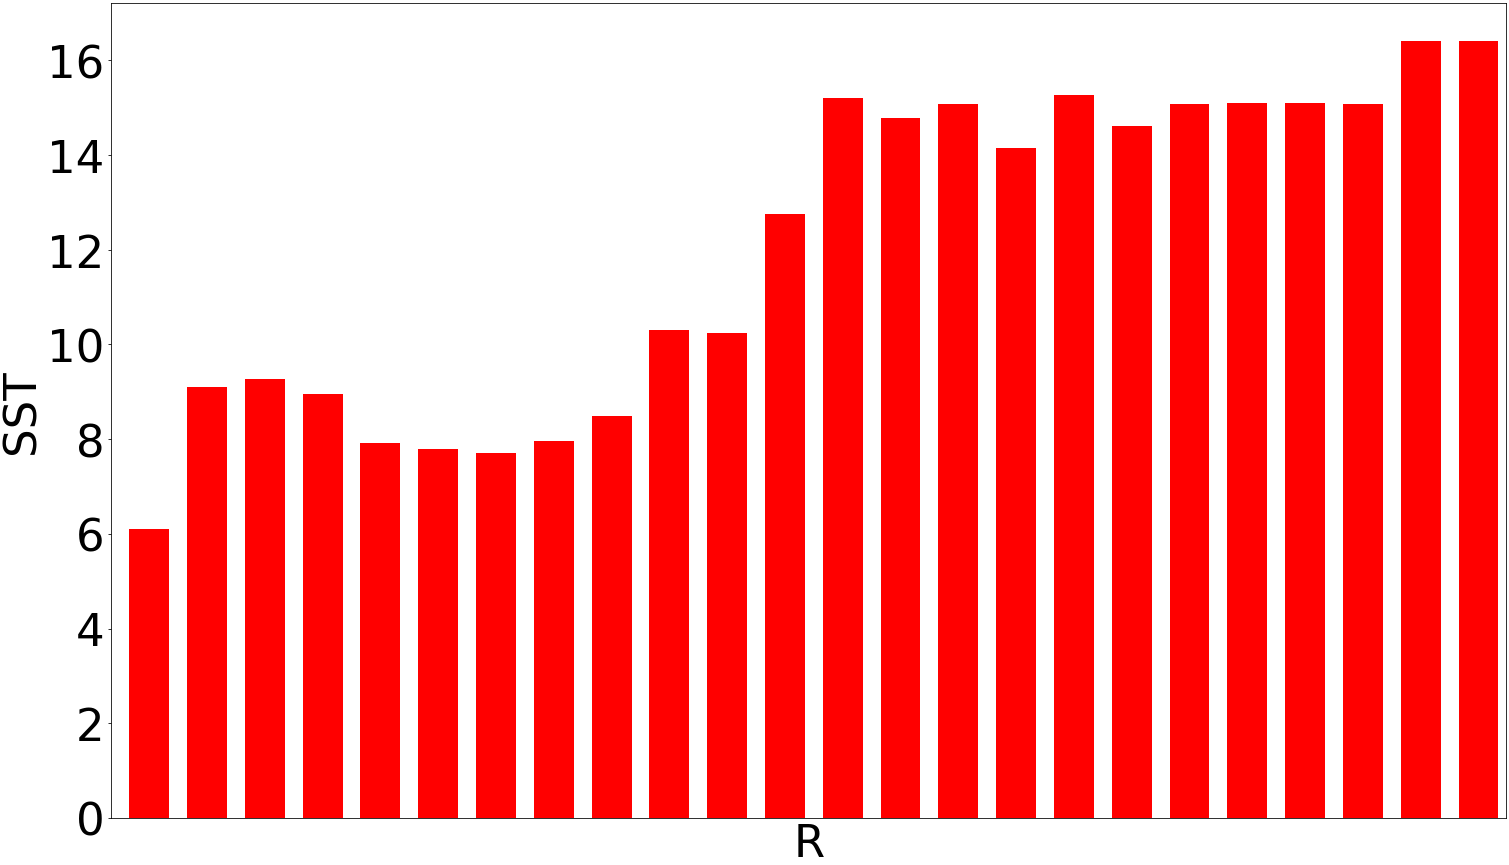
\includegraphics[scale=0.12]{img/R_sst_palmer.png}}
    \subcaptionbox{}{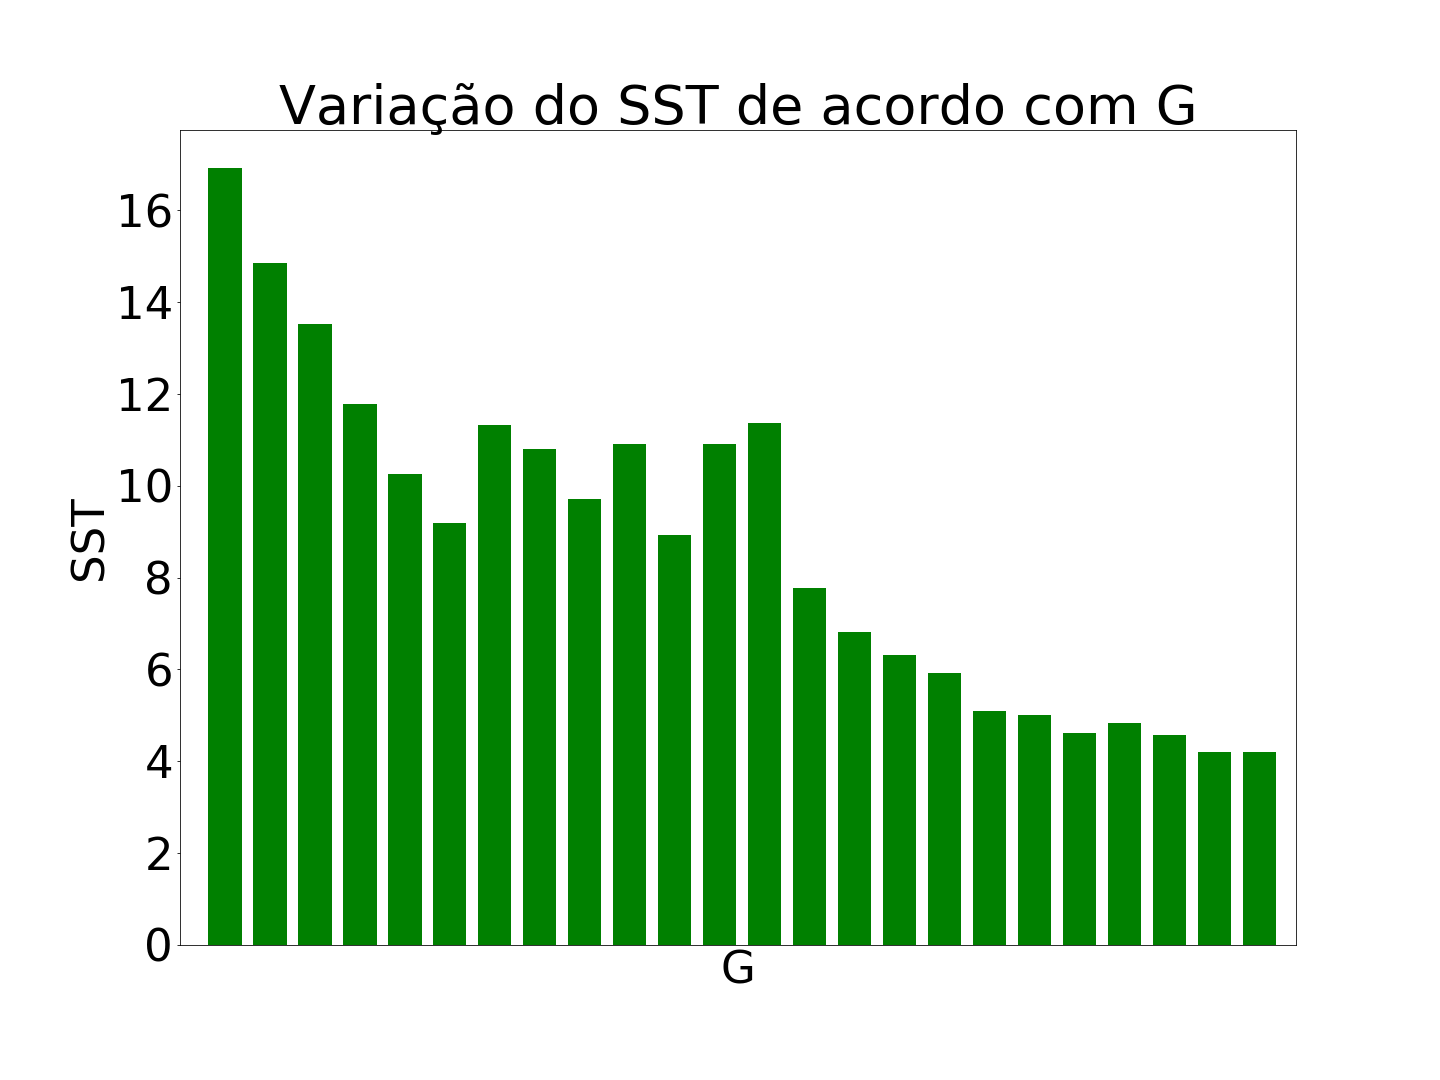
\includegraphics[scale=0.12]{img/G_sst_palmer.png}}
    \subcaptionbox{}{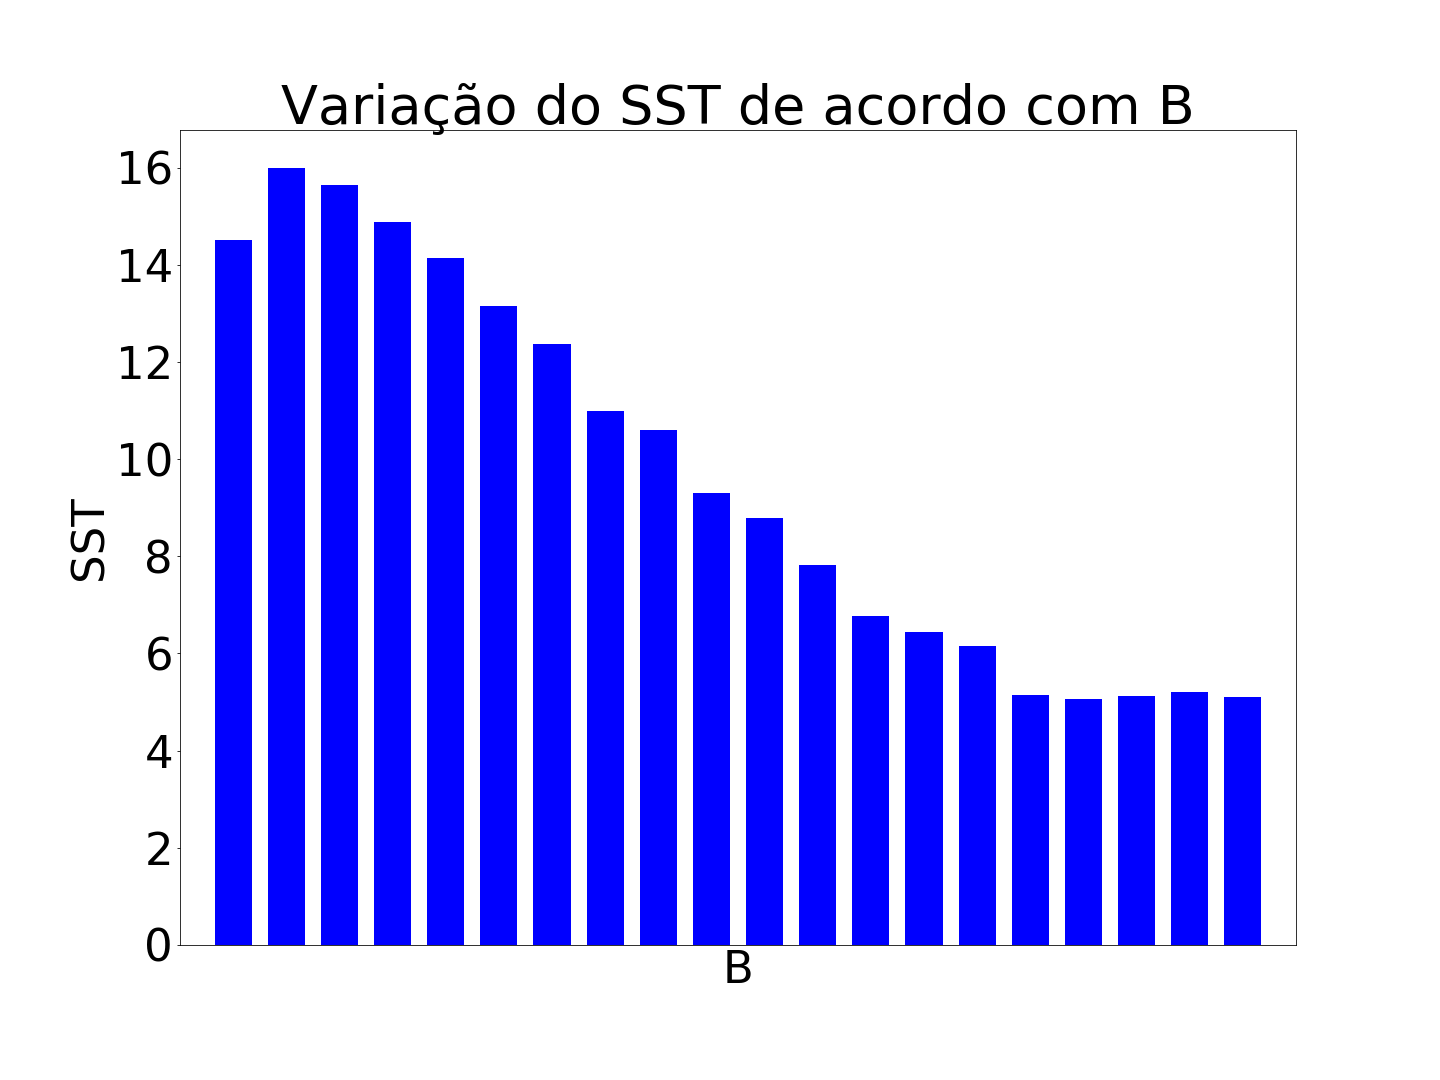
\includegraphics[scale=0.12]{img/B_sst_palmer.png}}
    \legend{\textbf{Fonte: } (Autor, 2019).}
\end{figure}

Nota-se um comportamento aproximadamente linear para as três variáveis. Assim, espera-se um resultado razoável para a Regressão Linear Múltipla, mas ainda melhor para a \textit{Random Forest}. Na Figura \ref{fig:fold_sst_rgb} são mostrados os valores de R e RMSE para a Regressão Linear e a técnica \textit{ensemble} em todos os \textit{folds}.

\begin{figure}[H]
\centering
	\caption{Métricas obtidas para cada \textit{fold}, obtidos para as duas técnicas de inferência (a) Coeficiente de correlação (R) (b) RMSE.}
	\subcaptionbox{}{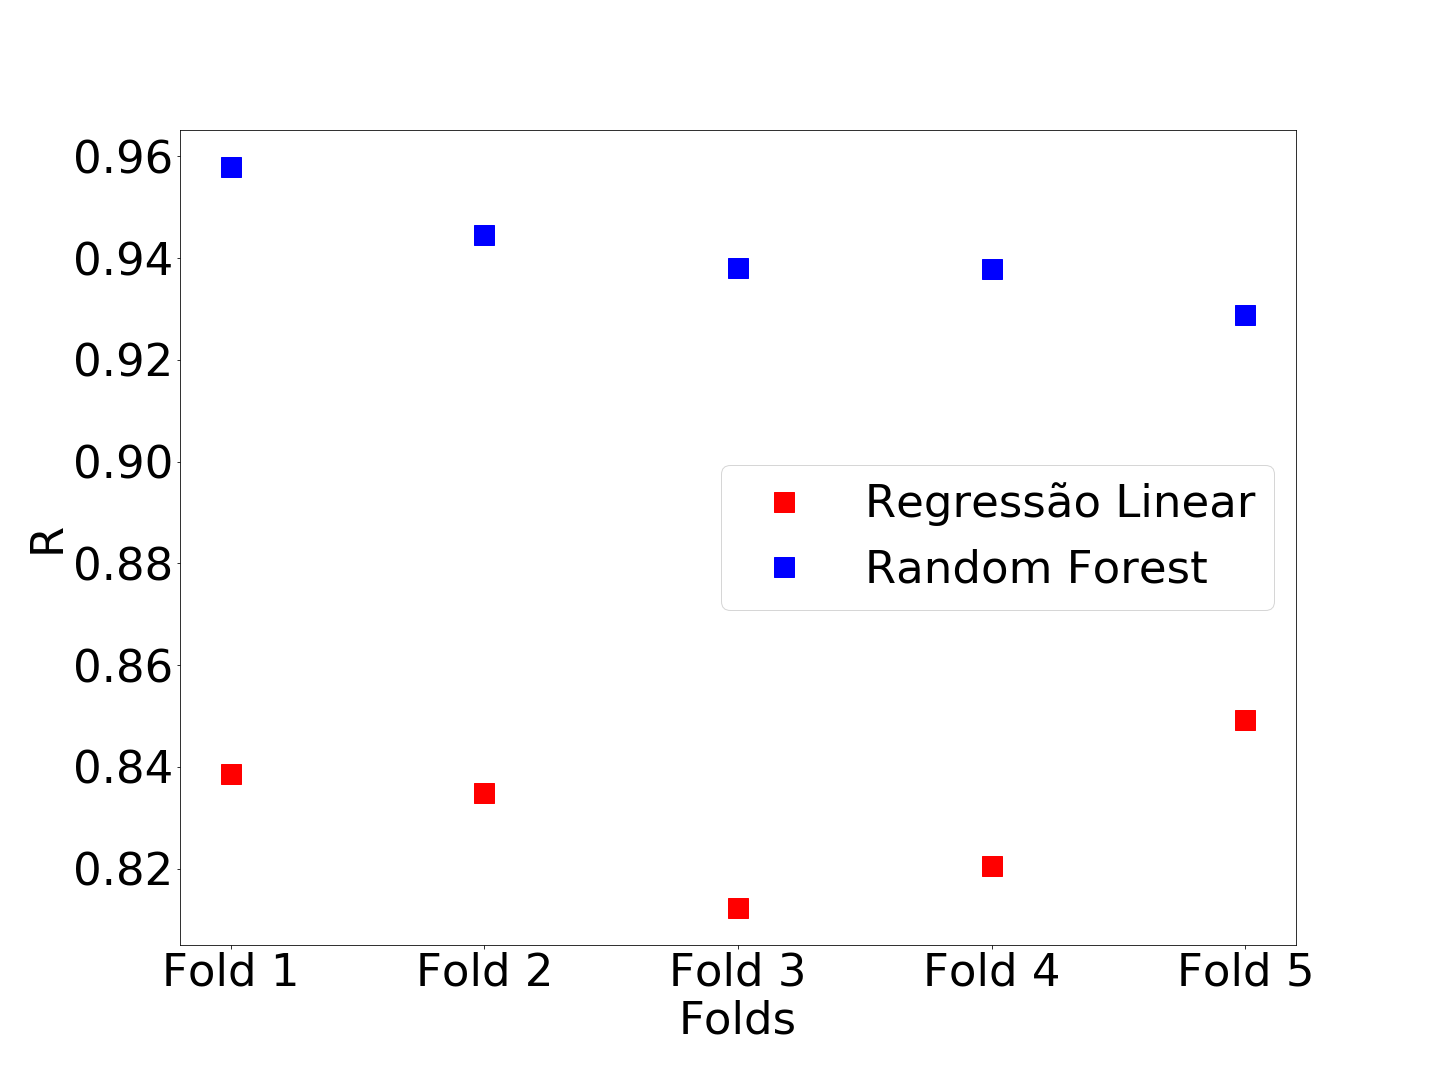
\includegraphics[scale=0.15]{img/fold_r_sst_rgb_palmer.png}}
	\subcaptionbox{}{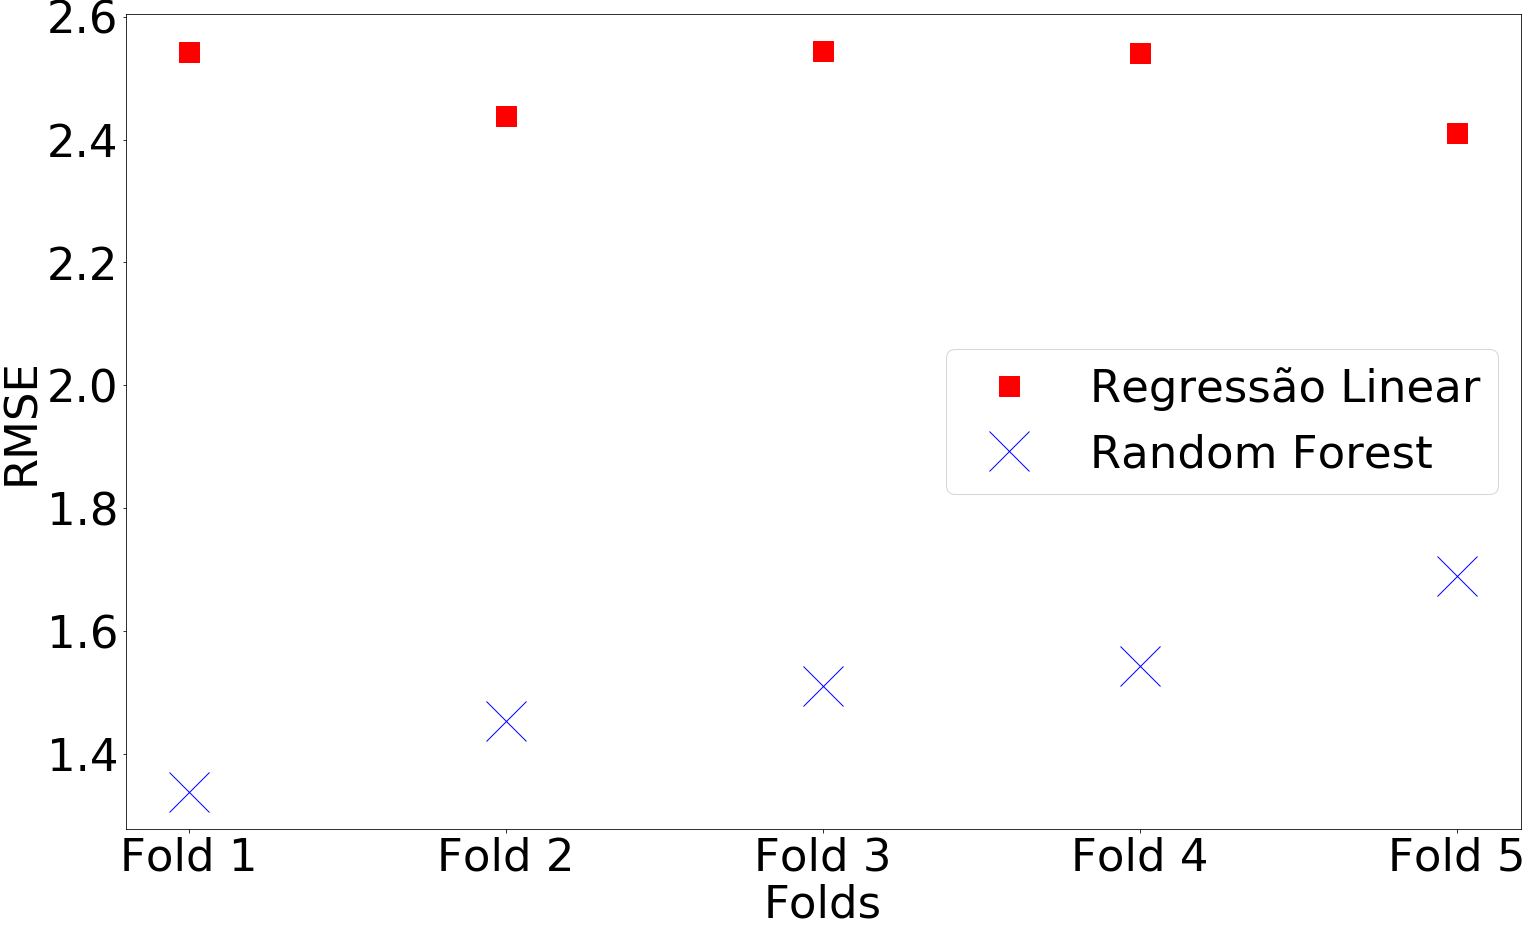
\includegraphics[scale=0.15]{img/fold_rmse_sst_rgb_palmer.png}}
	\legend{\textbf{Fonte:} (Autor, 2019).}\label{fig:fold_sst_rgb}
\end{figure}

Os valores médios dos coeficientes de correlação para a MLR e RF foram, respectivamente, iguais a 0,8312 e 0,9415. Ambas métricas mostraram-se superiores à obtida por Yahaya et al. (2015). Entretanto, o valor de RMSE obtido por eles ainda mostra-se menor que os alcançados para as mangas 'Palmer'. 

Desta forma, para a obtenção de um modelo que melhor explique a variação de SST, foi treinada uma \textit{Random Forest} com todas as variáveis listadas na Tabela \ref{tbl:var_gps}. Com um maior número de variáveis de entrada, há uma maior quantidade de informações associada à cada manga, aumentando-se assim a probabilidade de alcançar melhores resultados. Os valores de R e RMSE para cada \textit{fold} do modelo RF com todas as variáveis são mostrados na Tabela \ref{tbl:r_rmse_all}.

\begin{table}[H]
	\centering
	\caption{\label{tbl:r_rmse_all} Valores de R e RMSE obtidos para o modelo \textit{Random Forest} com todas as variáveis.}
	\begin{tabular}{lllll}
	\hline
	\multirow{2}{*}{\textit{Fold}} & \multicolumn{2}{c}{\textit{Random Forest}} & \multicolumn{2}{c}{Regressão Linear} \\ \cline{2-5}
	  	  & R      & RMSE    & R 	& RMSE\\ \hline
	1     & 0,9723 & 1,0018 & 0.9263 & 1.61544 \\ \hline
	2     & 0,9405 & 1,0987 & 0.9227 & 1.73668 \\ \hline
	3     & 0,9755 & 0,7075 & 0.9219 & 1.75353 \\ \hline
	4     & 0,9634 & 0,9029 & 0.9219 & 1.82808 \\ \hline
	5     & 0,9660 & 0,8104 & 0.9064 & 1.85705 \\ \hline
	Média & 0,9789 & 0,9042	& 0.9199 & 1.75816 \\ \hline
	\end{tabular}
	\legend{\textbf{Fonte: } (Autor, 2019).}
\end{table}

Nota-se mais uma vez que o modelo \textit{Random Forest} foi superior à Regressão Linear. O coeficiente de correlação obtido por ele foi maior que o encontrado pelos autores Khairunniza-Bejo e Kamarudin (2011) e Yahaya et al. (2015). Por outro lado, enquanto que o RMSE foi menor que o obtido por Yahaya et al. (2015), ainda foi maior que o RMSE encontrado por Khairunniza-Bejo e Kamarudin (2011) em seu trabalho.

Os atributos mais importantes para a determinação de SST em mangas 'Palmer' podem ser obtidos a partir da propriedade \textit{feature\_importances\_} do \textit{Scikit-Learn}, que retorna um valor de 0 a 1 para cada variável de entrada no modelo. Quanto mais próximo de 1 for o valor, mais importante a respectiva variável foi para a construção das regras de decisão da \textit{Random Forest}. Na Figura \ref{fig:feat_import} são mostradas as variáveis mais importantes do modelo.

\begin{figure}[H]
\centering
	\caption{Atributos mais importantes para a determinação de SST.}
	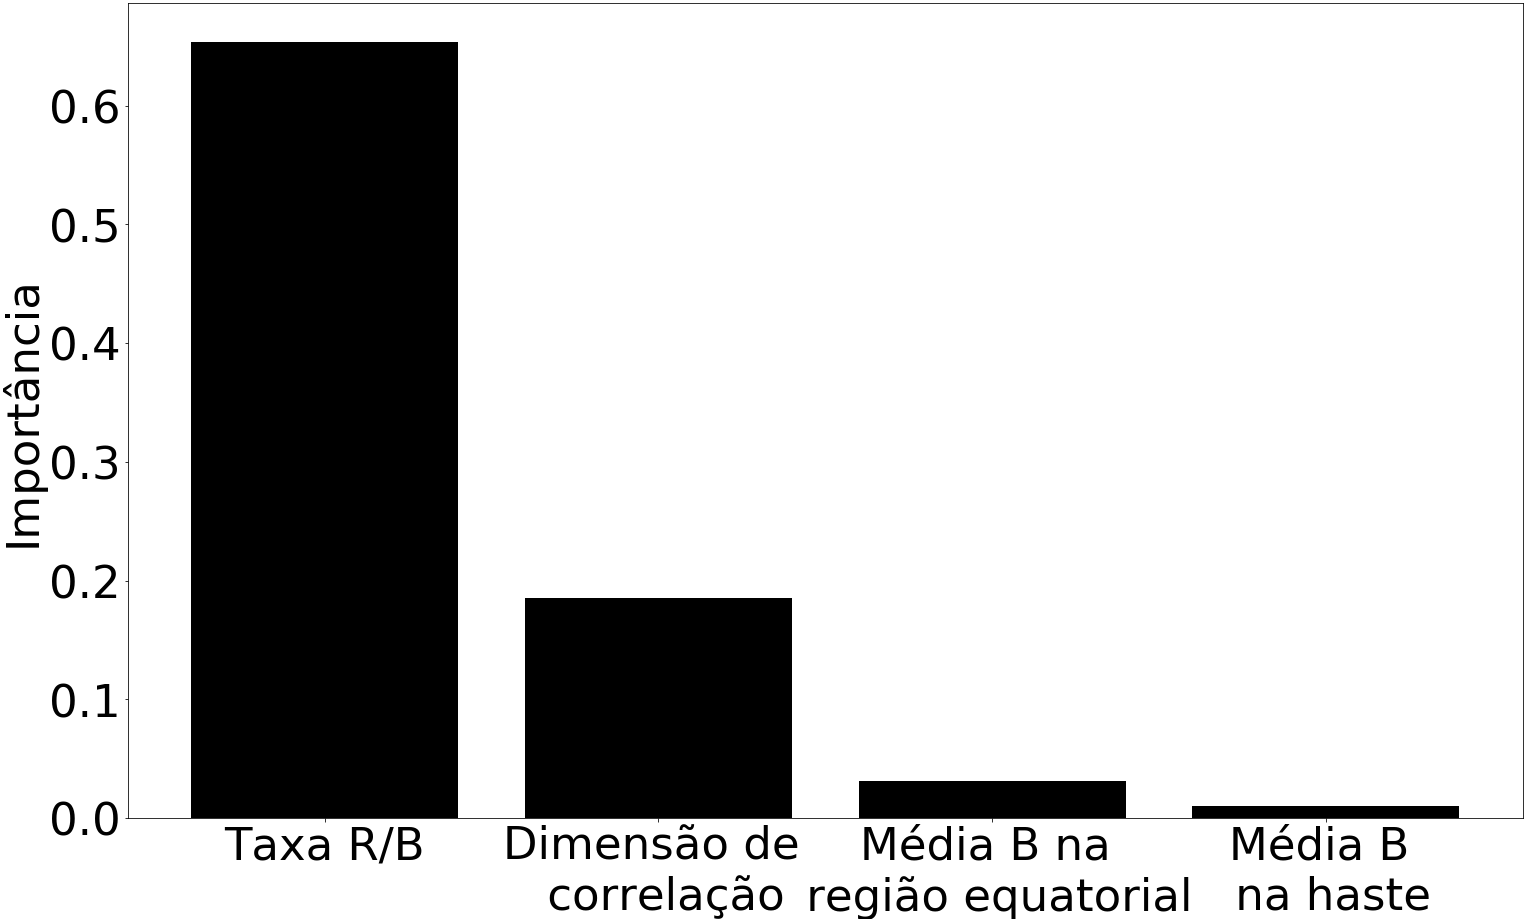
\includegraphics[scale=0.18]{img/feat_import_sst_palmer.png}
	\legend{\textbf{Fonte:} (Autor, 2019).}\label{fig:feat_import}
\end{figure}

Nota-se que o espaço de cores RGB, especialmente o canal B, foi o que mais possuiu relação com o SST. O atributo taxa R/B, que indica a razão entre o valor médio das intensidades no canal R e canal B, mostrou-se o mais significativo. A Figura \ref{fig:rbrate_fig} exibe uma foto em que as intensidades dos pixels originais foram convertidas para R/B. Nota-se, através dela, que a cor arroxeada/amarelada está fortemente associada aos sólidos solúveis totais.

\begin{figure}[H]
\centering
	\caption{Representação de uma foto no canal R/B.}
	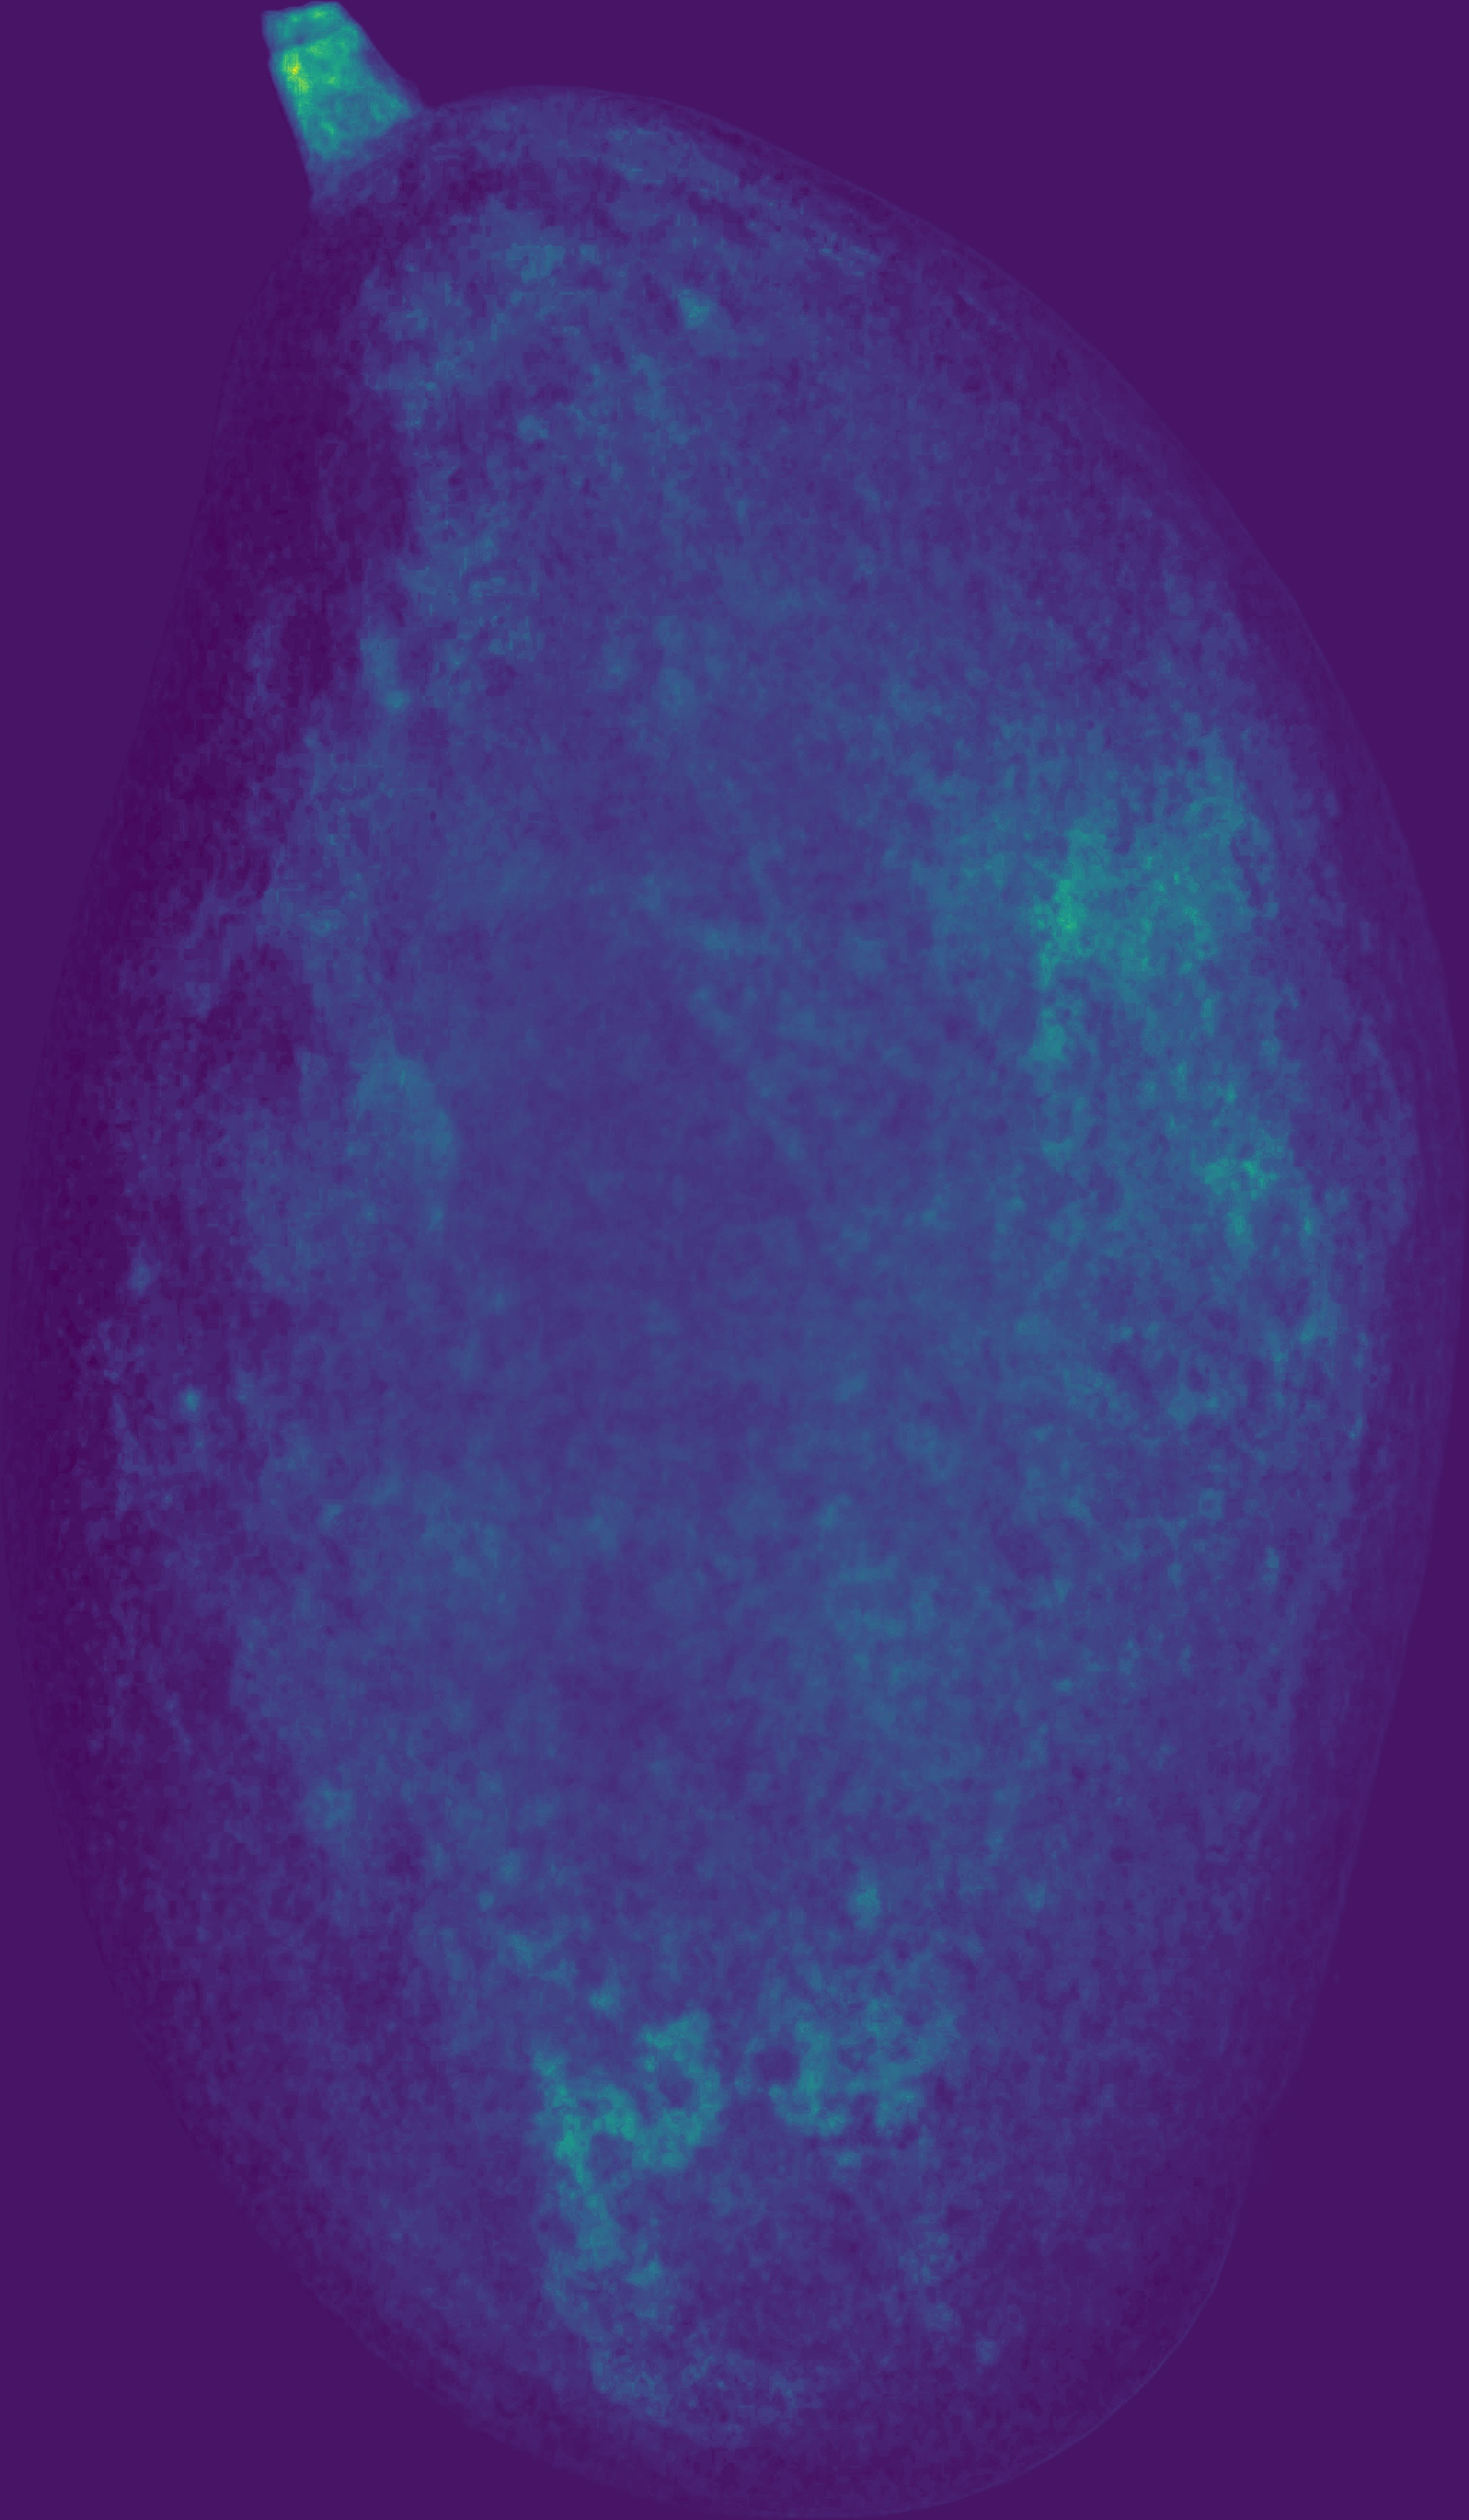
\includegraphics[scale=0.05]{img/RB_rate_img.jpg}
	\legend{\textbf{Fonte:} (Autor, 2019).}\label{fig:rbrate_fig}
\end{figure}

O atributo dimensão de correlação, o único dentre eles que não está associado à cor, estima o grau de desordem das intensidades dos pixels. Assim, o quão menos uniforme é a superfície da manga, maior a desordem. Ademais, os dois outros atributos são associados ao canal azul, em duas regiões específicas a manga. Na Figura \ref{fig:equator_stalk_b} são especificadas as regiões equatorial e da haste.

\begin{figure}[H]
\centering
	\caption{Regiões equatorial e haste em uma manga representada no canal B.}
	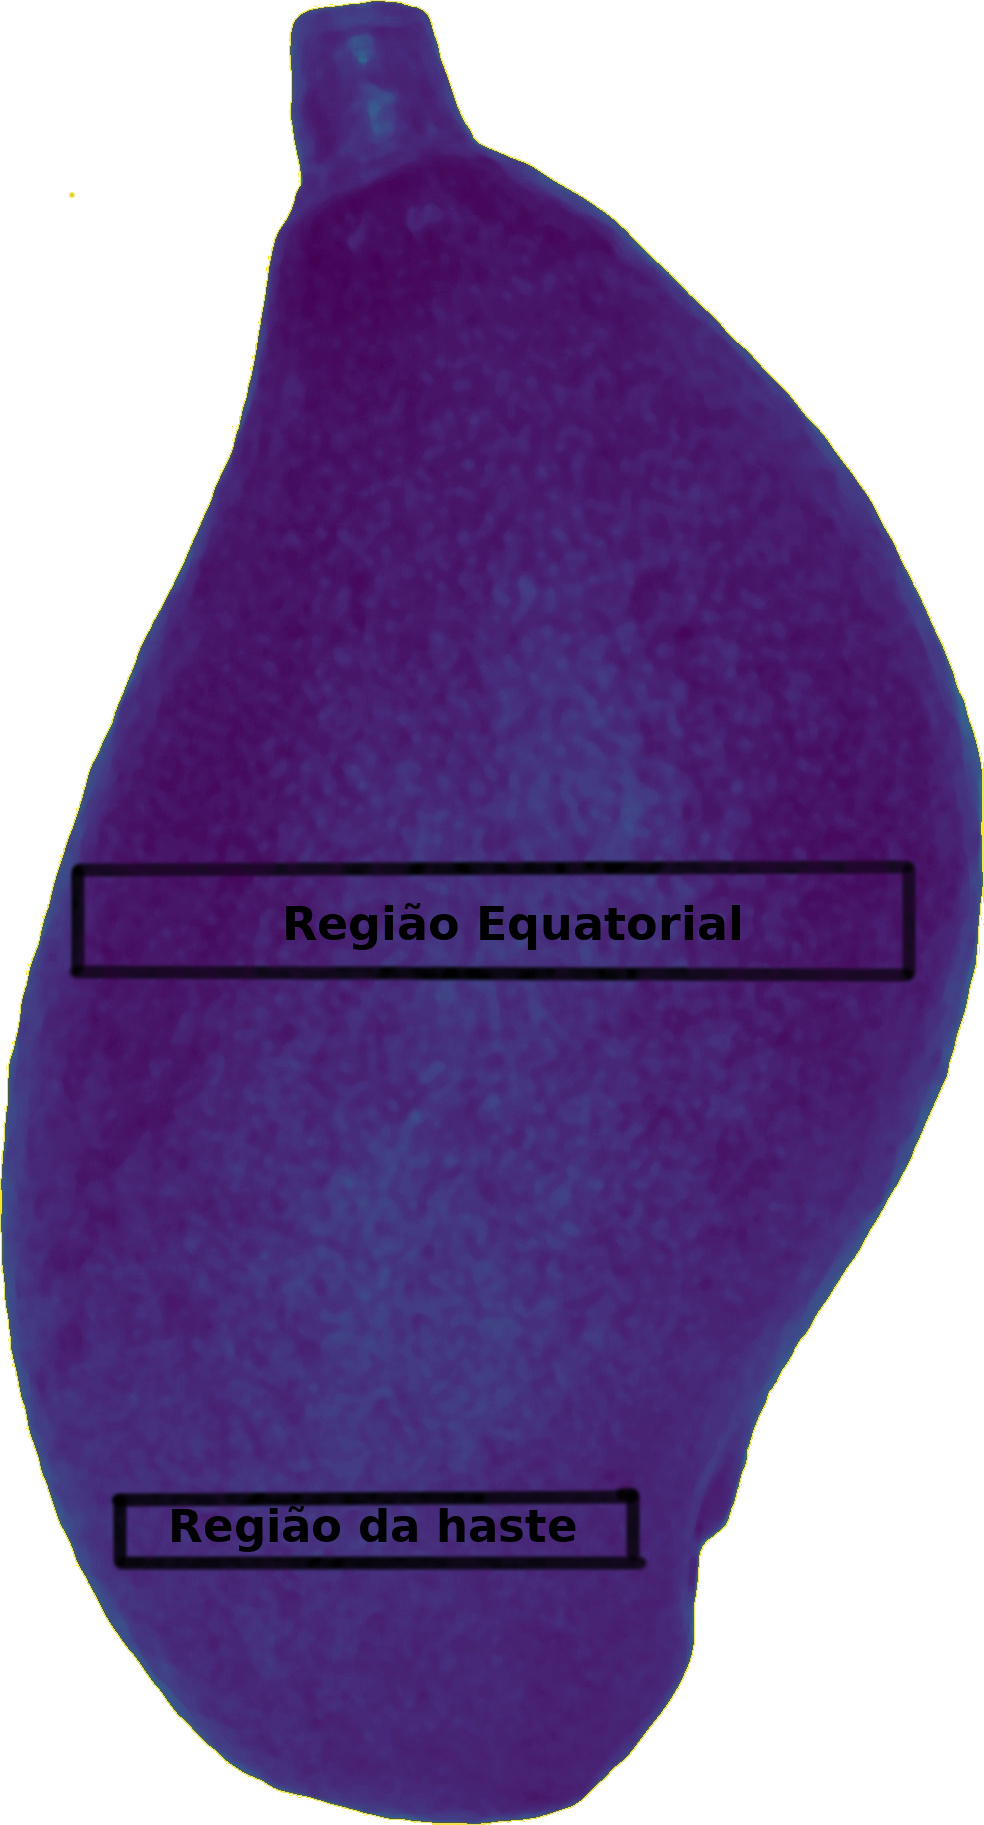
\includegraphics[scale=0.2]{img/B_img.jpg}
	\legend{\textbf{Fonte:} (Autor, 2019).}\label{fig:equator_stalk_b}
\end{figure}

Para entender a relação destas variáveis com o SST, foram plotadas as variações delas de acordo com o atributo de qualidade estudado, conforme mostra a Figura \ref{fig:var_atts}.

\begin{figure}[H]
\centering
	\caption{Variação dos atributos mais importantes para o modelo (a) Taxa R/B (b) Dimensão de correlação (c) Média B na região equatorial (d) Média B na região da haste.}
	\subcaptionbox{}{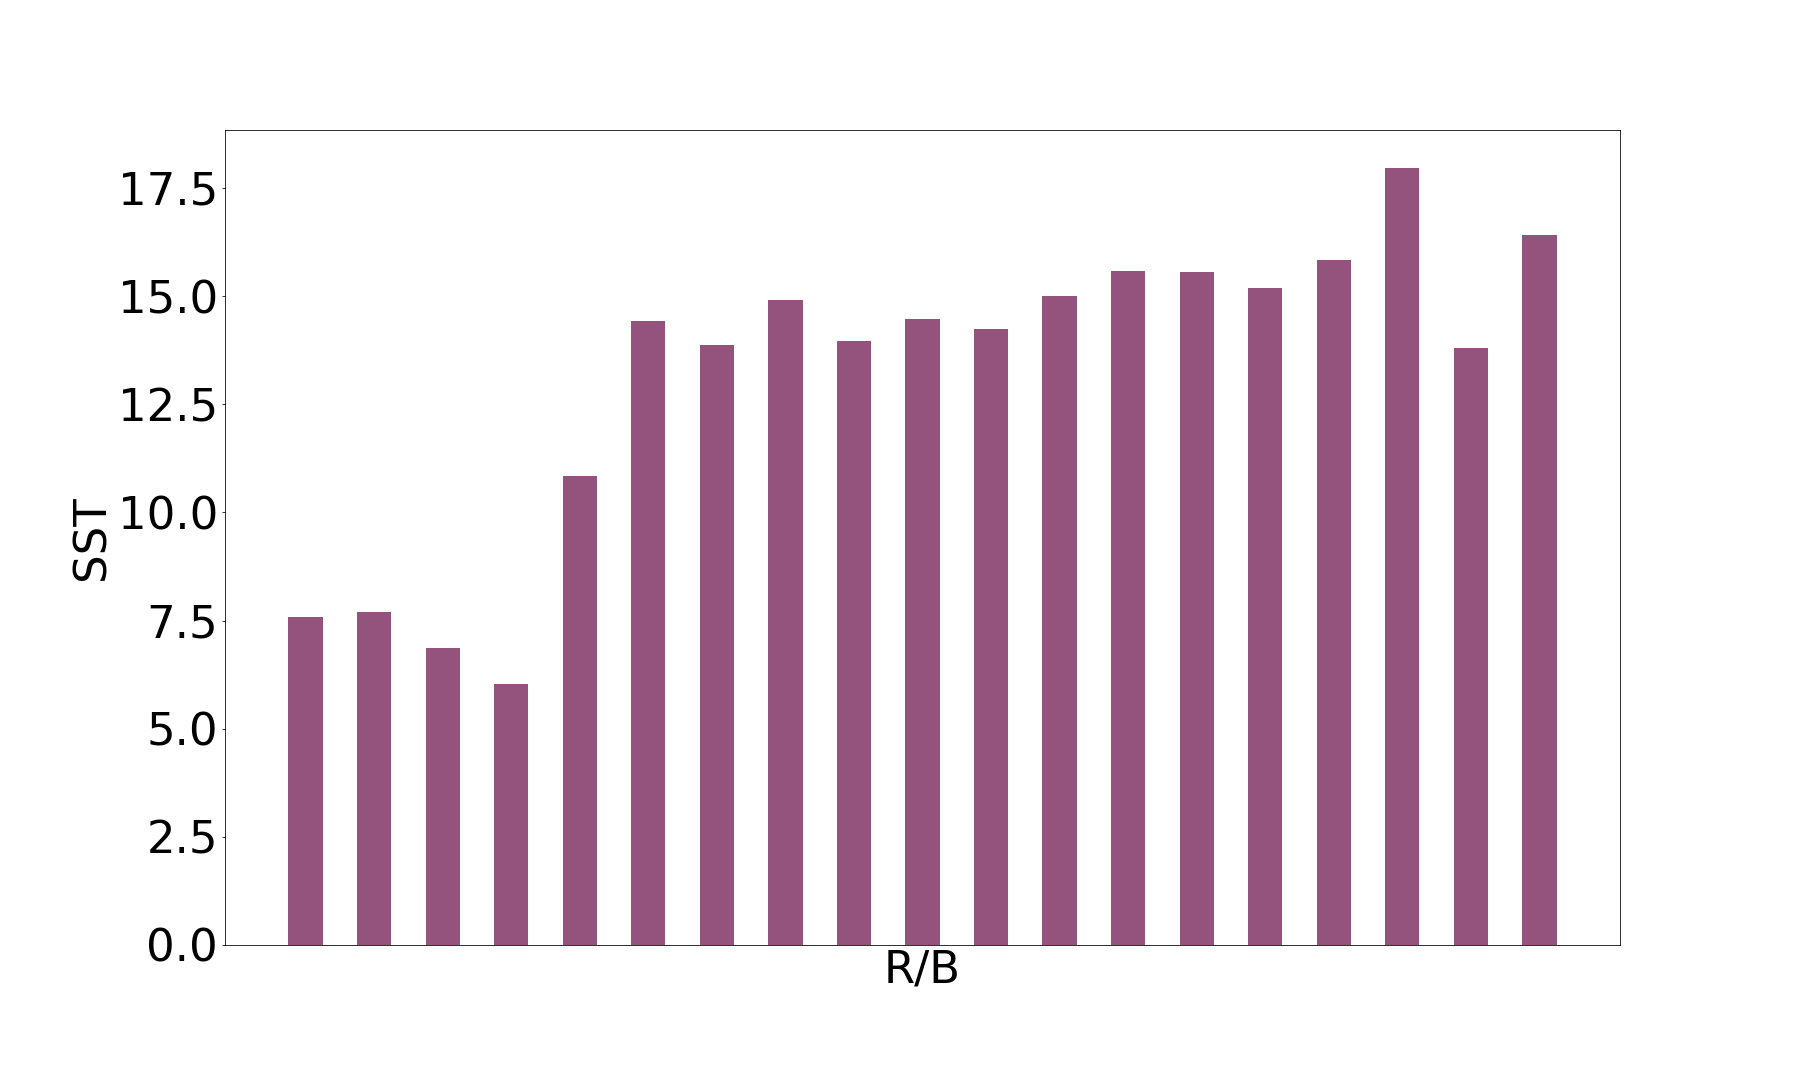
\includegraphics[scale=0.1]{img/RB_sst_palmer.png}}
	\subcaptionbox{}{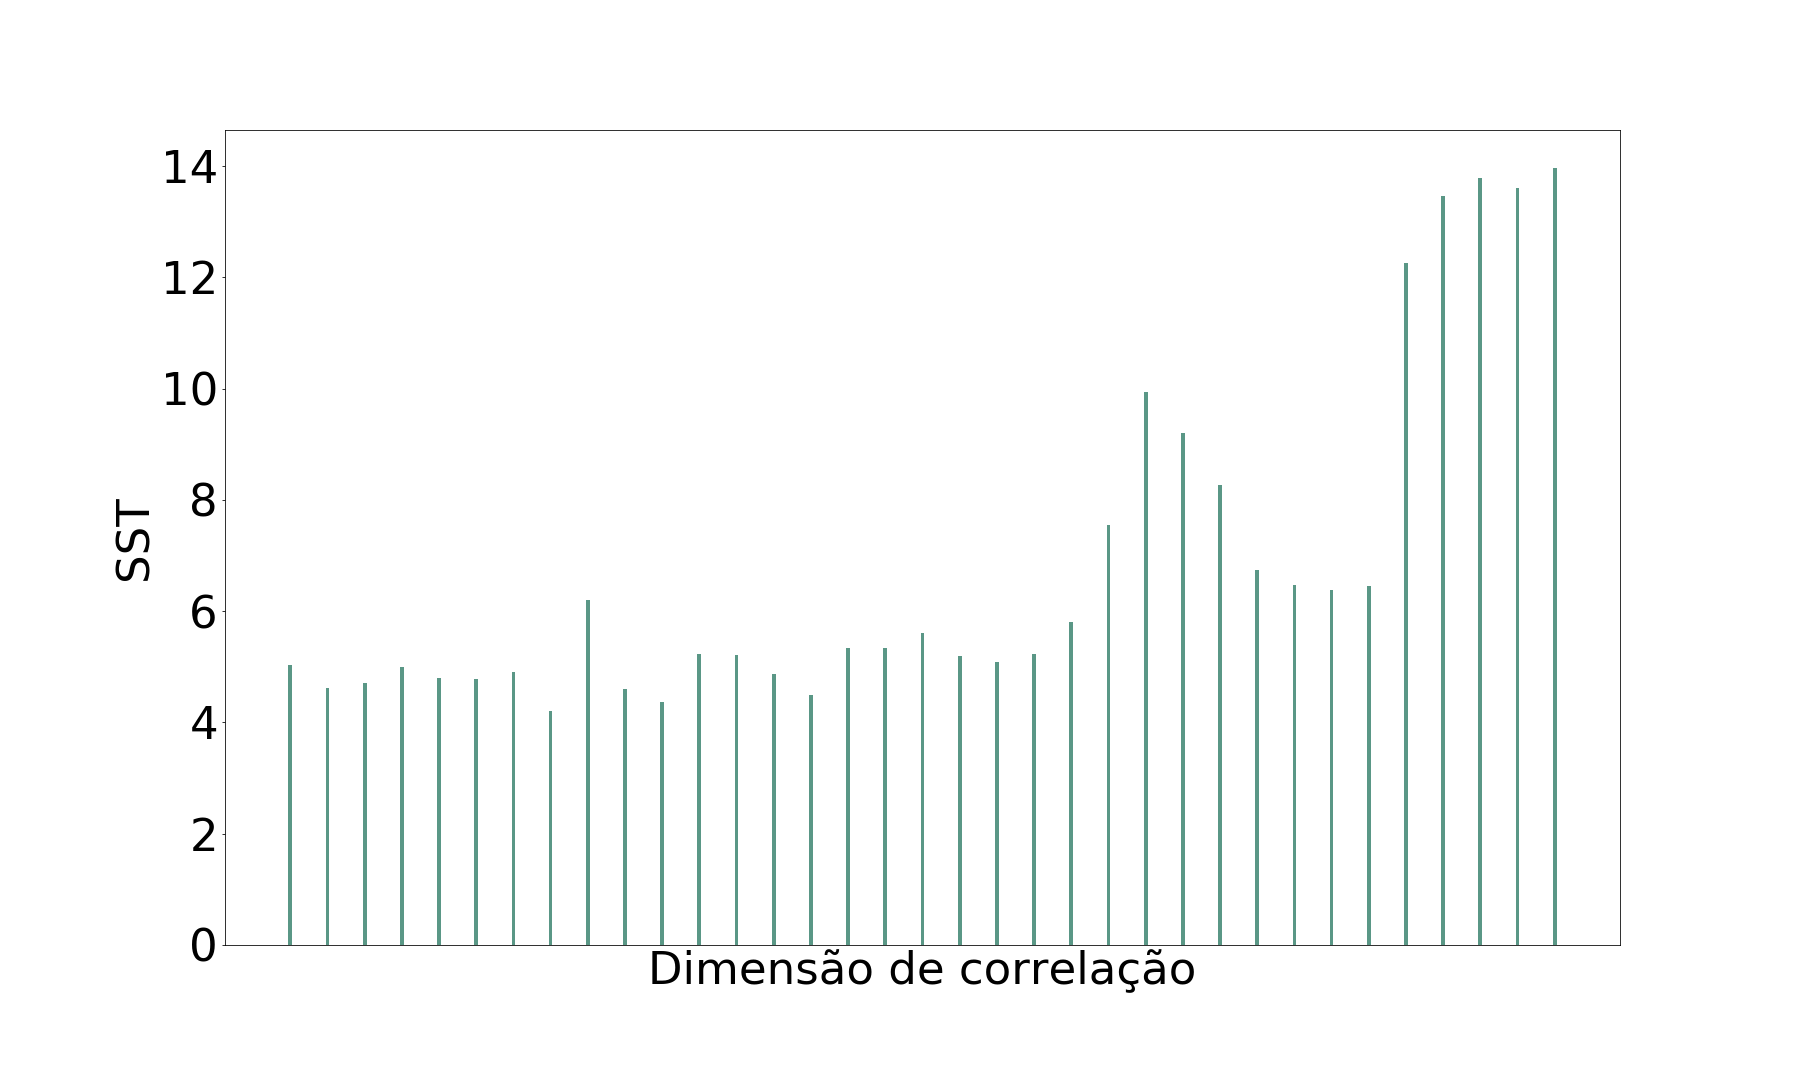
\includegraphics[scale=0.1]{img/cd_sst_palmer.png}}
	\subcaptionbox{}{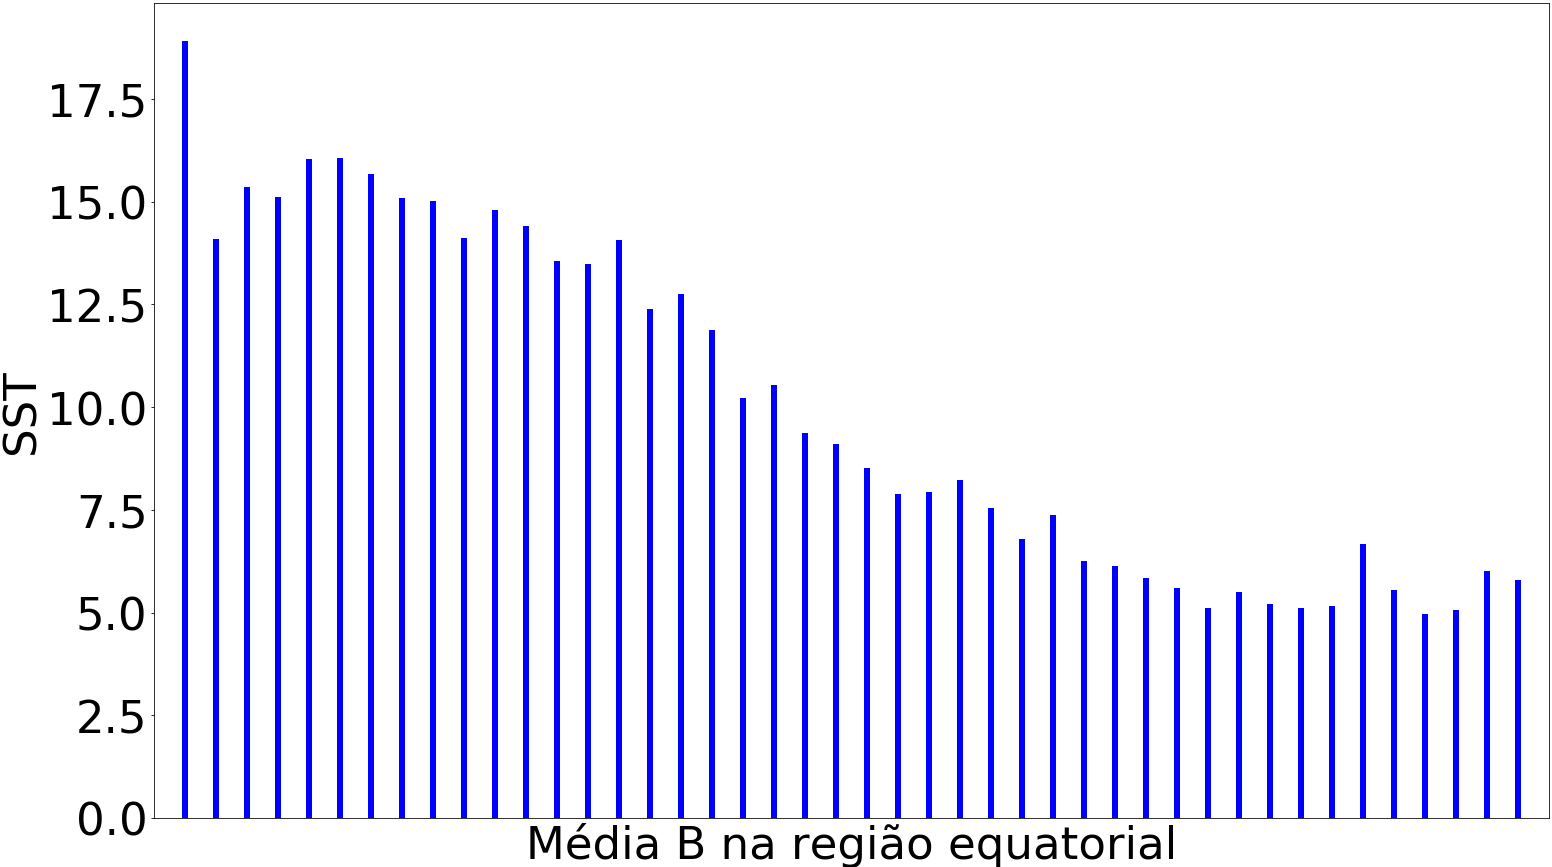
\includegraphics[scale=0.1]{img/equatorb_sst_palmer.png}}
	\subcaptionbox{}{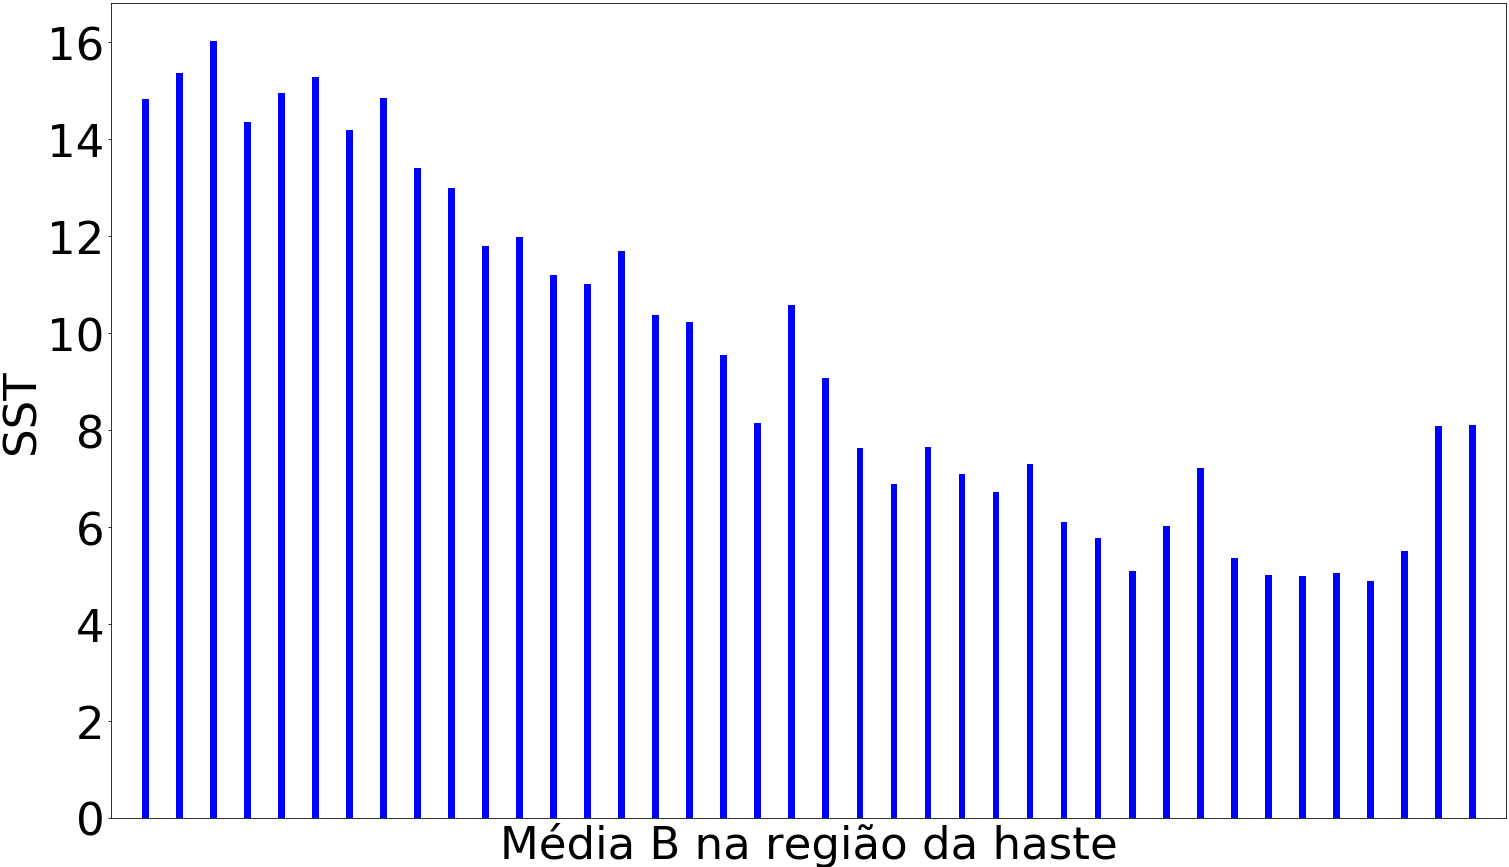
\includegraphics[scale=0.1]{img/stalkb_sst_palmer.png}}
	\legend{\textbf{Fonte:} (Autor, 2019).}\label{fig:var_atts}
\end{figure}

Para a primeira variável, percebe-se que seus valores mais baixos estão associados à mangas verdes, com baixo teor de SST. Com o aumento desse valor, aumenta-se gradativamente o SST, o que corresponde, na imagem, à uma diminuição dos tons amarelados e intensificação dos tons mais roxos. Para a dimensão de correlação, nota-se um comportamento pouco intuitivo e sem padrão, em que os valores de SST permanecem praticamente constantes para vários valores possíveis da dimensão de correlação. Nas outras duas variáveis, há uma diminuição perceptível do nível de SST enquanto a cor azul torna-se menos intensa nas respectivas regiões da manga.

Os demais atributos extraídos apresentaram importâncias menores que 0,01 e foram desconsiderados na construção de um novo modelo de \textit{Random Forest}, em que apenas as quatro variáveis mais importantes foram consideradas. O novo modelo apresentou um coeficiente de correlação igual a 0,9752, bastante próximo ao obtido para todas as variáveis.
% \section{Seção de exemplo 1 - Códigos} \label{sec:resex1}

% \subsection{Subseção de exemplo 1 - Inserindo trechos de códigos}
 
% O nosso querido Leonardo Cavalcante providenciou um comando que deixa nossos trechos de códigos bonitinhos e gera um elemento pré-textual de Lista de Códigos. 

% Os códigos são adicionados através do comando seguinte:

% \textbackslash sourcecode\{ Descrição \}\{Label\}\{Linguagem\}\{Arquivo com extensão\}

% Um exemplo pode ser visto no código \ref{cmd:cron} abaixo.

% \sourcecode{Configuração do intervalo de execução no Script Agendador}{cron}{javascript}{cron.js}


% \section{Seção de exemplo 2 - Listas} \label{sec:resex2}

% \subsection{Subseção de exemplo 2 - Lista de itens} 

% Existem alguns tipos de listas no Latex, iremos exemplificar a lista sem numeração (seção \ref{subsubsec:itemize}), a lista enumerada (seção \ref{subsubsec:enumerate}) e a lista mista (seção \ref{subsubsec:mista}). As listas podem ser encadeadas de diversas maneiras,
% de acordo com a necessidade do autor.

% \subsubsection{Subsubseção de exemplo 1 - Lista sem numeração} \label{subsubsec:itemize}

% Este é um exemplo de lista sem numeração.

% \begin{itemize}
% 	\item \textbf{Cadastrar usuário}

% 		\begin{itemize}
%     		\item Atores
% 		    	\begin{itemize}
%     		    	\item Usuário
% 		    	\end{itemize}

% 	    	\item Fluxo de eventos primário
% 			    \begin{itemize}
% 	    		    \item o usuário deve se cadastrar informando seu nome, \textit{e-mail} e senha;
% 		        	\item a API armazena os dados do usuário;
% 		    	    \item o usuário é liberado para realizar o \textit{login}.
% 			    \end{itemize}

%     		\item Fluxo alternativo
% 			    \begin{itemize}
% 		    	   \item o usuário desiste de se cadastrar e cancela o caso de uso clicando no botão voltar.
% 	    		\end{itemize}

% 		\end{itemize}
	
% \end{itemize}

% \subsubsection{Subsubseção de exemplo 2 - Lista enumerada} \label{subsubsec:enumerate}

% Este é um exemplo de lista enumerada.

% \begin{enumerate}
% 	\item O Usuário deseja ver o histórico das variáveis climáticas, então através da interface de usuário escolhe o período ao qual o histórico se refere;
% 	\item A aplicação solicita à API através de uma requisição HTTP contendo o momento de início e o momento do fim do período em seus parâmetros;     			\item A API recebe a solicitação e se comunica com a base de dados, então requere as informações quem possuem a data de leitura no intervalo escolhido;
% 	\item A base de dados retorna os dados em formato Json para a API;
% 	\item A API responde à requisição retornando os dados, também em formato Json, para a aplicação cliente;
% 	\item A aplicação cliente renderiza os gráficos utilizando o conjunto de dados obtidos.
% \end{enumerate}

% \subsubsection{Subsubseção de exemplo 3 - Lista mista} \label{subsubsec:mista}

% Este é um exemplo de lista mista.

% \begin{itemize}
% 	\item \textbf{Cadastrar usuário}

% 		\begin{itemize}
%     		\item Atores
% 		    	\begin{itemize}
%     		    	\item Usuário
% 		    	\end{itemize}

% 	    	\item Fluxo de eventos primário
% 			    \begin{enumerate}
% 	    		    \item o usuário deve se cadastrar informando seu nome, \textit{e-mail} e senha;
% 		        	\item a API armazena os dados do usuário;
% 		    	    \item o usuário é liberado para realizar o \textit{login}.
% 			    \end{enumerate}

%     		\item Fluxo alternativo
% 			    \begin{itemize}
% 		    	   \item o usuário desiste de se cadastrar e cancela o caso de uso clicando no botão voltar.
% 	    		\end{itemize}

% 		\end{itemize}

% 	\item \textbf{Visualizar dados atuais}

% 		\begin{itemize}
% 		    \item Atores
% 	    		\begin{itemize}
% 		    	    \item Usuário
% 			    \end{itemize}
    
% 	    	\item Pré-condições
% 			    \begin{itemize}
% 		     	   \item o usuário deve estar autenticado
% 			    \end{itemize}

% 	    	\item Fluxo de eventos primário
% 			    \begin{enumerate}
% 		    	    \item o usuário deve efetuar o \textit{login} informando o \textit{e-mail} e a senha;
% 	    		    \item caso o usuário não seja autenticado, o sistema informa a respeito de credenciais inválidas e encerra o caso de uso;
% 		    	    \item a API autentica o usuário;
%     			    \item o usuário é liberado para visualizar os dados atuais dos sensores da estação;
% 		        	\item após a visualização o usuário pode finalizar o caso de uso ou efetuar uma nova consulta se desejar.
% 			    \end{enumerate}

%     		\item Fluxo alternativo
% 			    \begin{itemize}
%     			   \item o usuário desiste de visualizar os dados atuais e cancela o caso de uso clicando no botão voltar.
% 			    \end{itemize}

% 		\end{itemize}

% 	\item \textbf{Visualizar histórico}

% 		\begin{itemize}
% 		    \item Atores
% 	    		\begin{itemize}
% 		    	    \item Usuário
% 	    		\end{itemize}

% 	    	\item Pré-condições
%     			\begin{itemize}
% 			        \item o usuário deve estar autenticado
% 			    \end{itemize}

% 		    \item Fluxo de eventos primário
% 			    \begin{enumerate}
% 			        \item o usuário deve efetuar o \textit{login} informando o \textit{e-mail} e a senha;
% 			        \item caso o usuário não seja autenticado, o sistema informa a respeito de credenciais inválidas e encerra o caso de uso;
% 			        \item a API autentica o usuário;
% 			        \item o usuário é liberado para escolher qual período cujo histórico será exibido;
% 			        \item o usuário seleciona as variáveis a serem exibidas no gráficos de linhas;
% 			        \item após a visualização do histórico o usuário pode finalizar o caso de uso se desejar.
% 			    \end{enumerate}

% 		    \item Fluxo alternativo
% 			    \begin{enumerate}
% 			        \item após a escolha do período de exibição do histórico o usuário pode voltar para a tela anterior e escolher um novo período;
% 			        \item o histórico é exibido para o usuário;
% 			        \item após a visualização do histórico o usuário pode finalizar o caso de uso ou efetuar uma nova consulta se desejar.
% 			    \end{enumerate}

% 		    \item Fluxo alternativo
% 			    \begin{enumerate}
% 			        \item o usuário desiste de visualizar o histórico e cancela o caso de uso clicando no botão voltar.
% 			    \end{enumerate}
% 		\end{itemize}
% \end{itemize}
		%--------------------------------------------------------------------------------------
% Este arquivo contém a sua conclusão
%--------------------------------------------------------------------------------------
\chapter{Considerações Finais e Trabalhos Futuros}

Com o teste de diferentes técnicas de pré-processamento, visando a maior redução possível de ruído, foi encontrado que as técnicas que proporcionaram um melhor resultado foram o filtro da mediana, as operações de abertura e fechamento, a limiarização simples e a segmentação de Otsu.

Com a extração de atributos e posterior construção dos modelos, concluiu-se que é possível determinar sólidos solúveis totais em mangas Palmer com um coeficiente de correlação igual a 0,9789, o maior encontrado na literatura. Enquanto que para os artigos pesquisados foi assumido um relacionamento linear entre as variáveis de entrada e a de saída, no presente estudo foi investigado se um modelo não linear comportaria-se melhor. Através dos resultados obtidos, concluiu-se que, de fato, um modelo não linear apresenta um desempenho melhor. Este resultado pode ser explicado através da inspeção dos atributos mais importantes, que não variam linearmente.

Verificou-se ainda que o espaço de cor mais significante para a determinação de SST é o RGB, em que o canal B se sobressai. A taxa R/B da imagem mostrou-se o mais importante, seguido do coeficiente de correlação e média do canal B nas regiões equatorial e da haste. A partir dessas quatro variáveis, construiu-se um novo modelo RF, em que o coeficiente de correlação foi igual a 0,9752.  
 
\section{Trabalhos futuros}

Através deste trabalho, determinou-se as técnicas de pré-processamento, atributos extraídos e algoritmo de predição que conferem o melhor resultado na determinação de sólidos solúveis totais em mangas da variedade Palmer. A partir disso, torna-se possível construir uma aplicação em que, a partir de uma foto tirada da manga, é determinado de forma não destrutiva o nível de SST na fruta. O ideal é que as fotos sejam tiradas em um ambiente controlado, da mesma forma em que foi realizado neste trabalho. Com o uso de um \textit{smartphone}, as fotos poderiam ser tiradas e enviadas a um servidor, que seria responsável por fazer o tratamento das imagens, extrair os quatro atributos mais significantes, obter o nível de SST através da \textit{Random Forest} e retornar este valor ao usuário.  

% \lipsum[55];
		\chapter{Referências}

\noindent ALVES, E. D. L.; VECCHIA, F. A. S. Análise de diferentes métodos de interpolação para a precipitação pluvial no Estado de Goiás. \textit{Acta Scientiarum. Human and Social Sciences}, v. 33, n. 2, 2011. Disponível em: <http://www.redalyc.org>. Acesso em: 01 ago. 2018.
\\

\noindent ABARRA, M. S. J. et al. Determination of Fruit Ripeness Degree of ‘Carabao’ Mango (Mangifera indica L.) using Digital Photometry. \textit{Philippine Journal of Science}, v. 147, n. 2, p. 249-253, 2018. Disponível em: <http://philjournalsci.dost.gov.ph/ >. Acesso em: 27 jun. 2018.
\\

\noindent ANUÁRIO BRASILEIRO DE FRUTICULTURA. Santa Cruz do Sul: Editora Gazeta, 2017. Disponível em: <http://www.editoragazeta.com.br>. Acesso em: 18 ago. 2018.
\\

\noindent ARCO, J. E. et al. Digital image analysis for automatic enumeration of malaria parasites using morphological operations. \textit{Expert Systems with Applications}, v. 42, n. 6, p. 3041-3047, 2015. Disponível em: <www.sciencedirect.com>. Acesso em: 29 jul. 2018.
\\

\noindent BEDI, S. S.; KHANDELWAL, Rati. Various image enhancement techniques-a critical review. \textit{International Journal of Advanced Research in Computer and Communication Engineering}, v. 2, n. 3, 2013. Disponível em: <https://pdfs.semanticscholar.org>. Acesso em: 29 jul. 2018.
\\

\noindent BRANCO, Danyelle Karine Santos et al. Comportamento das exportações de manga do Vale Submédio São Francisco: uma abordagem a partir de vetores autorregressivos. \textit{Revista Econômica do Nordeste}, v. 47, n. 4, p. 29-37, 2016. Disponível em: <https://www.bnb.gov.br>. Acesso em: 04 set. 2018.
\\

\noindent BREIMAN, L. Random forests. \textit{Machine learning}, v. 45, n. 1, p. 5-32, 2001.
\\

\noindent CAMASTRA, F. et al. A fuzzy decision system for genetically modified plant environmental risk assessment using Mamdani inference. \textit{Expert Systems with Applications}, v. 42, n. 3, p. 1710-1716, 2015.
\\

\noindent DA SILVA, L. A.; PERES, S. M.; BOSCARIOLI, C. \textit{Introdução à mineração de dados: com aplicações em R}. Elsevier Brasil, 2017.
\\

\noindent DE ABREU, A. L. E. \textit{Bootstrap e modelos de Support Vector Machine-SVM}. 2016. 117f. Dissertação (Doutorado em Métodos Numéricos) – Universidade Federal do Paraná, Curitiba, 2016. Disponível em: <www.acervodigital.ufpr.br>. Acesso em: 16 jul. 2018.
\\

\noindent DONIS-GONZÁLEZ, I. R. et al. Assessment of chestnut (Castanea spp.) slice quality using color images. \textit{Journal of Food Engineering}, v. 115, n. 3, p. 407-414, 2013. Disponível em: <www.sciencedirect.com>. Acesso em: 17 jun. 2018.
\\

\noindent DOMINGO, D. L. et al. Digital photometric method for determining degree of harvest maturity and ripeness of ‘Sinta’papaya (Carica papaya L.) fruits. \textit{The Philippine Agricultural Scientist}, v. 95, n. 3, 2013. Disponível em: <https://journals.uplb.edu.ph>. Acesso em: 18 jul. 2018.
\\

\noindent DORJ, U.; LEE, M.; YUN, S.. An yield estimation in citrus orchards via fruit detection and counting using image processing. \textit{Computers and Electronics in Agriculture}, v. 140, p. 103-112, 2017. Disponível em: <www.sciencedirect.com>. Acesso em: 27 jul. 2018.
\\

\noindent DOS SANTOS NETO, J. P. et al. Determination of ‘Palmer’mango maturity indices using portable near infrared (VIS-NIR) spectrometer. \textit{Postharvest Biology and Technology}, v. 130, p. 75-80, 2017. Disponível em: <www.sciencedirect.com>. Acesso em: 02 jul. 2018. 
\\

\noindent DUARTE FILHO, J. et al. Aspectos do florescimento e técnicas empregadas objetivando a produção precoce em morangueiros. \textit{Informe Agropecuário}, v. 20, n. 198, p. 30-35, 1999. 
\\

\noindent EMBRAPA SEMIÁRIDO. \textit{Cultivo da mangueira}. Petrolina, 2002. Disponível em: <https://ainfo.cnptia.embrapa.br>. Acesso em: 08 ago. 2018.
\\

\noindent ENVI - Guia do ENVI em Português. Sulsoft, 2000. Diponível em: <www.sulsoft.com.br>. Acesso em: 17 jul. 2018.
\\

\noindent ESQUEF, A. \textit{Técnicas de entropia em processamento de imagens}. RIO DE JANEIRO: CENTRO BRASILEIRO DE PESQUISAS FÍSICAS, 2002.
\\

\noindent FERRAZ, M. N. \textit{Uso da espectrometria para investigação da qualidade da cana-de-açúcar em campo.}2015. 148 p. Dissertação (Mestrado em Engenharia de Sistemas Agrícolas) - Universidade de São Paulo, Piracicaba, 2015.
\\

\noindent FONSECA, J. J. S. Metodologia da pesquisa científica. Fortaleza: UEC, 2002. Apostila.
\\

\noindent FRIEDMAN, Jerome; HASTIE, Trevor; TIBSHIRANI, Robert. \textit{The elements of statistical learning}. New York, NY, USA:: Springer series in statistics, 2001.
\\

\noindent GAMA, João et al. \textit{Extração de conhecimento de dados: data mining}. 2015.
\\

\noindent GIL, A. C. Como elaborar projetos de pesquisa. 4. ed. São Paulo: Atlas, 2007.
\\

\noindent GONZALEZ, R. C.; WOODS, R. C. \textit{Processamento digital de imagens}. Pearson Educación, 2009.
\\

\noindent HAYKIN, S. \textit{Redes neurais: princípios e prática}. Porto Alegre: Bookman, 2001. 900 p.
\\

\noindent HEMALATHA, G.; SUMATHI, C. P. Preprocessing techniques of facial image with Median and Gabor filters. In: \textit{Information Communication and Embedded Systems (ICICES), 2016 International Conference on}. IEEE, 2016. p. 1-6. Disponível em: <https://ieeexplore.ieee.org>. Acesso em: 29 jul. 2018.
\\

\noindent HUTENGS, C.; VOHLAND, M. Downscaling land surface temperatures at regional scales with random forest regression. \textit{Remote Sensing of Environment}, v. 178, p. 127-141, 2016. Disponível em: <www.sciencedirect.com>. Acesso em: 02 ago. 2018.
\\

\noindent IAL - INSTITUTO ADOLFO LUTZ. \textit{Métodos físico-químicos para análise de alimentos}. São Paulo, 2008. 1020 p.
\\

\noindent IMAGE THRESHOLDING. OpenCV. Disponível em: <https://docs.opencv.org/3.4/d7/d4d/tutorial\_py\_thresholding.html>. Acesso em: 17 feb. 2019.
\\

\noindent JAMES, Gareth et al. \textit{An introduction to statistical learning}. New York: springer, 2013.
\\

\noindent JATMIKA, S.; PURNAMASARI, D.. Rancang Bangun Alat Pendeteksi Kematangan Buah Apel dengan Menggunakan Metode Image Processing Berdasarkan Komposisi WARNA. \textit{Jurnal Ilmiah Teknologi Informasi Asia}, v. 8, n. 1, p. 51-58, 2014. Disponível em: <https://jurnal.stmikasia.ac.id>. Acesso em: 18 jul. 2018.
\\

\noindent JHA, S. N.; KINGSLY, A. R. P.; CHOPRA, Sangeeta. Physical and mechanical properties of mango during growth and storage for determination of maturity. \textit{Journal of Food engineering}, v. 72, n. 1, p. 73-76, 2006. Disponível em: <www.sciencedirect.com>. Acesso em: 02 jul. 2018.
\\

\noindent JOSEPH, R. P.; SINGH, C. S.; MANIKANDAN, M. Brain tumor MRI image segmentation and detection in image processing. International \textit{Journal of Research in Engineering and Technology}, v. 3, n. 1, p. 1-5, 2014. Disponível em: <https://s3.amazonaws.com>. Acesso em: 18 jul. 2018.
\\

\noindent KAUR, A.; KRANTHI, B. V. Comparison between YCbCr color space and CIELab color space for skin color segmentation. \textit{IJAIS}, v. 3, n. 4, p. 30-33, 2012. Disponível em: <https://pdfs.semanticscholar.org>. Acesso em: 29 jul. 2018.
\\

\noindent KHAIRUNNIZA-BEJO, S.; KAMARUDIN, S. Chokanan mango sweetness determination using hsb color space. In: \textit{Computational Intelligence, Modelling and Simulation (CIMSiM), 2011 Third International Conference on}. IEEE, 2011. p. 216-221. Disponível em: <www.ieeexplore.ieee.org>. Acesso em: 13 jun. 2018.
\\

\noindent MIHALOVIC, M. Performance comparison of multiple discriminant analysis and logit models in bankruptcy prediction. \textit{Economics \& Sociology}, v. 9, n. 4, p. 101, 2016. Disponível em: <http://www.economics-sociology.eu>. Acesso em: 17 jul. 2018.
\\

\noindent MORPHOLOGICAL TRANSFORMATIONS. OpenCV-Python Tutorials. Disponível em: <https://opencv-python-tutroals.readthedocs.io/en/latest/py\_tutorials/py\_imgproc/py\_morphological\_ops/py\_morphological\_ops.html>. Acesso em: 17 jul. 2018.
\\

\noindent 2-D MEDIAN FILTERING. MathWorks Inc. Disponível em: <https://www.mathworks.com/help/images/ref/medfilt2.html>. Acesso em: 17 jul. 2018.
\\

\noindent NADAFZADEH, M.; MEHDIZADEH, S. A.; SOLTANIKAZEMI, M. Development of computer vision system to predict peroxidase and polyphenol oxidase enzymes to evaluate the process of banana peel browning using genetic programming modeling. \textit{Scientia Horticulturae}, v. 231, p. 201-209, 2018. Disponível em: <www.sciencedirect.com>. Acesso em: 27 jul. 2018.
\\

\noindent NANDI, C. S.; TUDU, B.; KOLEY, C. A machine vision-based maturity prediction system for sorting of harvested mangoes. \textit{IEEE Transactions on Instrumentation and measurement}, v. 63, n. 7, p. 1722-1730, 2014. Disponível em: <https://ieeexplore.ieee.org>. Acesso em: 12 jun. 2018.
\\

\noindent NETO, F. P. L. Novas opções de variedades de mangueira e as vantagens competitivas. In: \textit{Embrapa Semiárido-Artigo em anais de congresso (ALICE). In: FEIRA NACIONAL DA AGRICULTURA IRRIGADA-FENAGRI, 20.}, 2009. Disponível em: <www.alice.cnptia.embrapa.br>. Acesso em: 31 jul. 2018.
\\

\noindent PAM – \textit{Produção Agrícola Municipal}. Disponível em: <https://sidra.ibge.gov.br/pesquisa/pam>. Acesso em: 08 ago. 2018.
\\

\noindent PANDEY, R.; GAMIT, N.; NAIK, S. Non-destructive quality grading of mango (Mangifera Indica L) based on CIELab colour model and size. In: \textit{Advanced Communication Control and Computing Technologies (ICACCCT), 2014 International Conference on}. IEEE, 2014. p. 1246-1251. Disponível em: <http://ieeexplore.ieee.org>. Acesso em: 27 jun. 2018.
\\

\noindent PERMADI, Y. et al. Aplikasi Pengolahan Citra Untuk Identifikasi Kematangan Mentimun Berdasarkan Tekstur Kulit Buah Menggunakan Metode Ekstraksi Ciri Statistik. \textit{Jurnal Informatika}, v. 9, n. 1, 2015. Disponível em: <http://www.journal.uad.ac.id>. Acesso em: 18 jul. 2018.
\\

\noindent PRAVEEN, K. S. et al. Implementation Of Image Sharpening And Smoothing Using Filters. \textit{International Journal of Scientific Engineering and Applied Science}, v. 2, n. 1, p. 7-14, 2016. Disponível em: <http://ijseas.com>. Acesso em: 29 jul. 2018.
\\

\noindent RUSSELL, Stuart J.; NORVIG, Peter. \textit{Artificial intelligence: a modern approach}. Malaysia; Pearson Education Limited,, 2016.
\\

\noindent SALUNKHE, R., P.; PATIL, A. A. Image processing for mango ripening stage detection: RGB and HSV method. In: \textit{Image Information Processing (ICIIP), 2015 Third International Conference on}. IEEE, 2015. p. 362-365. Disponível em: <https://ieeexplore.ieee.org/>. Acesso em: 13 jun. 2018.
\\

\noindent SCHMUTZLER, M.; HUCK, C. W. Simultaneous detection of total antioxidant capacity and total soluble solids content by Fourier transform near-infrared (FT-NIR) spectroscopy: a quick and sensitive method for on-site analyses of apples. \textit{Food Control}, v. 66, p. 27-37, 2016.
\\

\noindent SHAIK, K. B. et al. Comparative study of skin color detection and segmentation in HSV and YCbCr color space. \textit{Procedia Computer Science}, v. 57, p. 41-48, 2015. Disponível em: <www.sciencedirect.com >. Acesso em: 17 jul. 2018.
\\

\noindent SONKA, M.; HLAVAC, V.; BOYLE, R. \textit{Image processing, analysis, and machine vision}. Cengage Learning, 2014.
\\

\noindent TEOH, C. C.; SYAIFUDIN, A. R. M. Image processing and analysis techniques for estimating weight of Chokanan mangoes. \textit{Journal of Tropical Agriculture and Food Science}, v. 35, n. 1, p. 183, 2007. Disponível em: <http://ejtafs.mardi.gov.my/jtafs/35-1/Chokanan\%20mangoes.pdf>. Acesso em: 11 jun. 2018.
\\

\noindent VÉLEZ-RIVERA, N. et al. Computer vision system applied to classification of “Manila” mangoes during ripening process. \textit{Food and bioprocess technology}, v. 7, n. 4, p. 1183-1194, 2014. Disponível em: <https://link.springer.com/article/10.1007/s11947-013-1142-4>. Acesso em: 11 jun. 2018.
\\

\noindent YADAV, S.; JAIN, C.; CHUGH, A.. Evaluation of image deblurring techniques. \textit{Evaluation}, v. 139, n. 12, 2016. Disponível em: <www.pdfs.semanticscholar.org >. Acesso em: 16 jul. 2018.
\\

\noindent YAHAYA, O. K. M. et al. Determining Sala mango qualities with the use of RGB images captured by a mobile phone camera. In: \textit{AIP Conference Proceedings}. AIP Publishing, 2015. p. 060003. Disponível em: <http://aip.scitation.org>. Acesso em: 27 jun. 2018.
\\

\noindent YOSSY, E. H. et al. Mango Fruit Sortation System using Neural Network and Computer Vis
ion. \textit{Procedia Computer Science}, v. 116, p. 596-603, 2017. Disponível em: <www.sciencedirect.com>. Acesso em: 13 jun. 2018.
\\

\noindent ZHENG, H.; LU, H. A least-squares support vector machine (LS-SVM) based on fractal analysis and CIELab parameters for the detection of browning degree on mango (Mangifera indica L.). \textit{Computers and Electronics in Agriculture}, v. 83, p. 47-51, 2012. Disponível em: <www.sciencedirect.com>. Acesso em 12 jun. 2018.

	\postextual
		% \bibliography{tex/references}
		\begin{anexosenv}
\chapter{\textit{Strings} de busca empregadas} \label{anex:anexo1}

Os dez artigos estudados foram obtidos após buscas no \textit{Google Scholar}, onde foram utilizadas diferentes \textit{strings}, conforme mostra a Tabela abaixo. 

\begin{center}
\scalefont{0.85}
\begin{longtable}{ll}
\caption{\textit{Strings} de busca pesquisadas e artigos encontrados.}\\
\hline
\multicolumn{1}{c}{\textit{String}} & \multicolumn{1}{c}{Artigos} \\ \hline
\endfirsthead

\endhead

\endfoot

\endlastfoot

% \textbf{TESTE}                            & Envia a \textit{string} "TEST\textbackslash n" de volta  \\ \hline
% \textbf{WRD}                        & Responde com o tipo de estação meteorológica \\ \hline
% \textbf{RXCHECK}                        & Responde com o diagnóstico do Console \\ \hline
% \textbf{RXTEST}                       & Muda a tela do console de \textit{"Receiving from"} para tela de dados atuais                                                        \\ \hline
% \textbf{VER}                           & Responde com a data do \textit{firmware}                                                             \\ \hline
% \textbf{RECEIVERS}                    & Responde com a lista das estações que o console "enxerga" \\ \hline
% \textbf{NVER}                       & Responde com a versão do \textit{firmware}                                                             \\ \hline
% \textbf{LOOP}                     & Responde com a quantidade de pacotes especificada a cada 2s        \\ \hline
% \textbf{LPS}                & Responde a cada 2s com a quantidade de pacotes diferentes especificada          \\ \hline
% \textbf{HILOWS}                & Responde com todo os dados de \textit{high/low}                 \\ \hline
% \textbf{PUTRAIN}                      & Seta a quantidade anual de precipitação \\ \hline
% \textbf{PUTET}                 & Seta a quantidade anual de evapotranspiração        \\ \hline
% \textbf{DMP}                 & Faz o \textit{download} de todo o arquivo de memória \\ \hline
% \textbf{DMAFT}                   & Faz o \textit{download} de todo o arquivo de memória após a data especificada \\ \hline
% \textbf{GETEE}                 & Lê toda a memória EEPROM \\ \hline
% \textbf{EEWR}                   & Escreve um \textit{byte} de dados à partir do endereço especificado                                   \\ \hline
% \textbf{EERD}                   & Lê a quantidade de dados especificada iniciando no endereço especificado                                   \\ \hline
% \textbf{EEBWR}                   & Escreve os dados na EEPROM                                    \\ \hline
% \textbf{EEBRD}                   & Lê os dados da EEPROM \\ \hline
% \textbf{CALED}                 & Envia os dados da temperatura e umidade corrente para atribuir à calibração \\ \hline
% \textbf{CALFIX}                   & Atualiza o \textit{display} quando os números de calibração mudam\\ \hline
% \textbf{BAR}                   & Seta os valores da elevação e o \textit{offset} do barômetro quando a localização é alterada                                   \\ \hline
% \textbf{BARDATA}                   & Mostra os valores atuais da calibração do barômetro                                   \\ \hline \\
% \textbf{CLRLOG}                 & Limpa todo o arquivo de dados                                                       \\ \hline
% \textbf{CLRALM}                   & Limpa todos os limiares dos alarmes                                   \\ \hline
% \textbf{CLRCAL}                   & Limpa todos os \textit{offsets} da calibração da temperatura e da umidade \\ \hline
% \textbf{CLRGRA}                   & Limpa o gráfico do console \\ \hline
% \textbf{CLRVAR}                   & Limpa o valor da precipitação ou da evapotranspiração \\ \hline
% \textbf{CLRHIGHS}                   & Limpa todos os valores de pico diários, mensais ou anuais                                   \\ \hline
% \textbf{CLRLOWS}                   & Limpa todos os valores de mínimos diários, mensais ou anuais \\ \hline
% \textbf{CLRBITS}                   & Limpa os \textit{bits} de alarme ativos                                  \\ \hline
% \textbf{CLRDATA}                   & Limpa todos os dados atuais                                   \\ \hline
% \textbf{BAUD}                 & Atribui o valor do \textit{baudrate} do console                                                       \\ \hline
% \textbf{SETTIME}                   & Define a data e a hora do console                                   \\ \hline
% \textbf{GAIN}                   & Define o ganho do receptor de rádio                                   \\ \hline
% \textbf{GETTIME}                   & Retorna a hora e a data atual do console                                   \\ \hline
% \textbf{SETPER}                   & Define o intervalo de arquivamento                                   \\ \hline
% \textbf{STOP}                   & Desabilita a criação dos registros                                   \\ \hline
% \textbf{START}                   & Habilita a criação dos arquivos \\ \hline
% \textbf{NEWSETUP}                   & Reinicia o console após alguma configuração nova                                  \\ \hline
% \textbf{LAMPS}                   & Liga ou desliga as lâmpadas do console \\ \hline

\textit{Mango image processing}				& - \textit{Image processing and analysis techniques for estimating weight} \\
											& \textit{of Chokanan mangoes} \\ 
											& - \textit{A least-squares support vector machine (LS-SVM) based on fractal}  \\ 
											& \textit{analysis and CIElab paramaters for the detection of browning degree} \\ 
											& \textit{on mango (Mangifera indica L.)} \\ \hline

\textit{Mango image processing maturity}	& - \textit{A machine vision-based maturity prediction system for sorting of} \\
											&	\textit{harvested mangoes} \\ \hline

\textit{Mango camera sugar content}			& - \textit{Chokanan mango sweetness determination using HSB color space} \\ \hline

\textit{Mango classification} 				& - \textit{Computer vision system applied to classification of “Manila”} \\
											& 	\textit{mangoes during ripening process} \\ \hline

\textit{Mango HSV}							& - \textit{Mango Fruit Sortation System using Neural Network and Computer} \\
											& 	\textit{Vision} \\ \hline

\textit{Mango RGB}							& - \textit{Image Processing for Mango Ripening Stage Detection: RGB and} \\
											&	\textit{HSV method} \\ 
											& - \textit{Non-Destructive Quality Grading Of Mango (Mangifera Indica L)} \\
											&	\textit{Based On CIELAB Colour Model and Size}  \\
											& - \textit{Determination of Fruit Ripeness Degree of ‘Carabao’ Mango} \\
											&	\textit{(Mangifera indica L.) using Digital Photometry} 	\\
											& - \textit{Determining Sala Mango Qualities with the use of RGB Images} \\
											&	\textit{Captured by a Mobile Phone Camera} \\ \hline

%\label{tab:6}
\end{longtable}
\legend{\textbf{Fonte: } (Autor, 2019).}
\end{center}


\end{anexosenv}


\end{document}
